In an attempt to answer \ref{rq:1}, 
this chapter presents a proposal for the engineering of \acp{DT}
focusing on the challenges of integrating heterogeneous sources of \ac{PA} data
and exposing \ac{DT} functionalities as services for digital applications.
%
Additionally, the chapter addresses the challenge of managing the \emph{lifecycle} of a \ac{DT}, 
which is crucial to ensure that the \ac{DT} can accurately reflect the state of the \ac{PA}, 
or signal when it may not be able to do so, in order for applications to make informed decisions on how to 
interpret the data provided by the \ac{DT}.
%
Finally, the modelling of \emph{augmented} functionalities of a \ac{DT} is discussed, with a modular approach
in order to decouple them from the primary \ac{DT} responsibility of \emph{shadowing} the \ac{PA} state. 
%
The resulting contribution is the proposal of an architectural framework and patterns for the engineering of \acp{DT}, 
which has been implemented in a supporting open-source framework: the \ac{WLDT} Java Library\footnote{\url{https://wldt.github.io}}.

%=======================================================
\section{An Abstract Architecture for \aclp{DT}}
\label{sec:dte:engineering-dt:abstract-architecture}
%=======================================================
Starting from the principles outlined by the 5D model~\cite{dt-driven-prognostics-tao-2018},
and incorporating insights from both recent academic research~\cite{web-of-dt-ricci-2022,Bellavista_Bicocchi_Fogli_Giannelli_Mamei_Picone_2023} and relevant standards from industry bodies~\cite{etsi-dt-comm-requirements-2024}.
This section presents a proposal aiming to generalize an abstract architecture that captures the core software requirements for \ac{DT} development.

%%%
\begin{figure}[t]
    \centering
    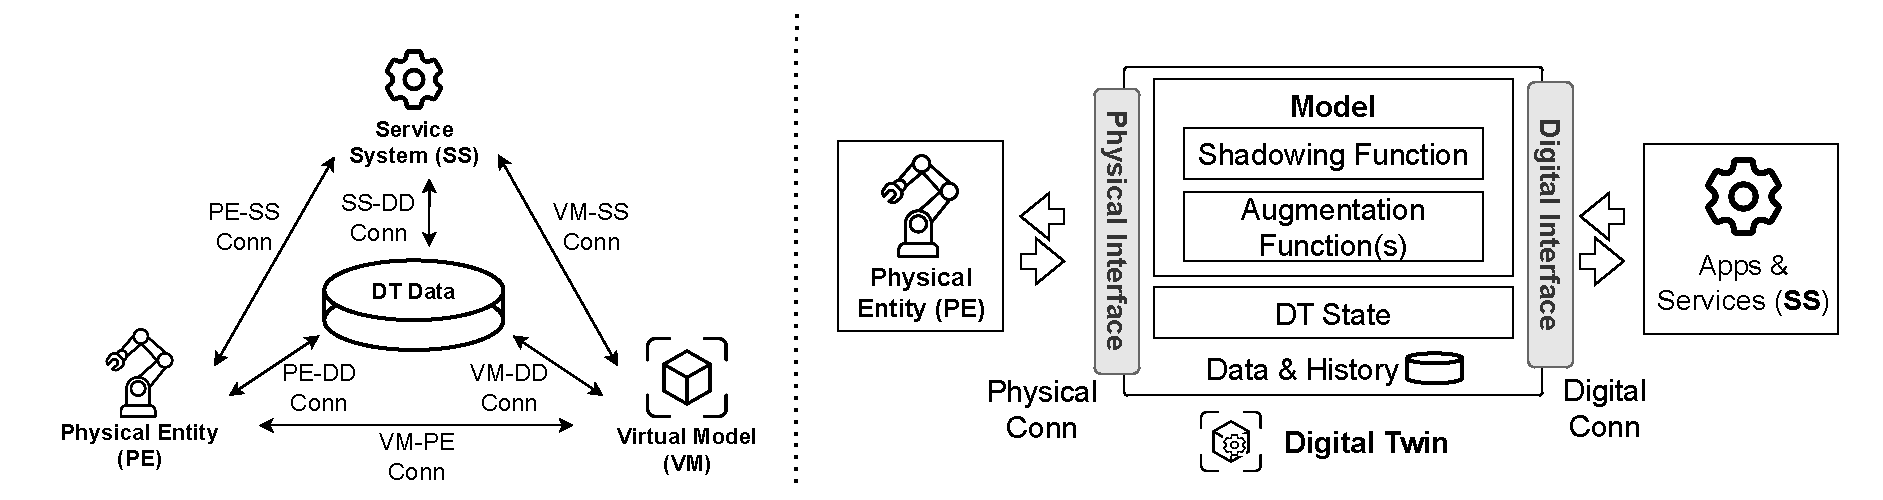
\includegraphics[width=\textwidth]{figures/mapping-Tao-WLDT.pdf}
    \caption{A side-by-side mapping between 5D DT modelling and the abstract \ac{DT} architecture.}
    \label{fig:tao_mapping_dt_modelling}
\end{figure}
%%%

In the 5D model (Figure \ref{fig:tao_mapping_dt_modelling}, left), 
the first dimension, Physical Entities (PE), represents the actual physical object or system being modeled as a \ac{DT}.
The second dimension, Virtual Entity (VE), is the digital representation of the physical entity, replicating its characteristics and behaviors.
The third dimension, Connection (C), ensures linkage between the physical and virtual entities, including communication technologies, data transmission protocols, and synchronization mechanisms for real-time interaction and data exchange.
The fourth dimension, Data (D), covers data management aspects, ensuring accurate and timely data for simulation, prediction, and optimization.
Finally, the fifth dimension, Service (S), involves various services enabled by the \ac{DT}, such as monitoring, simulation, prediction, control, and optimization, leveraging data and insights from the virtual entity to enhance the performance and efficiency of the physical system.

Moving this towards an abstract architectural perspective, a \ac{DT} can be described as the combination of three main high-level components as schematically illustrated in Figure \ref{fig:tao_mapping_dt_modelling} (right): 

\begin{itemize}
    \item \textit{\ac{PI}:} tasked with both the digitalization process and the ongoing synchronization of the \ac{DT} and \ac{PA} throughout their lifecycle based on its characteristic cyber-physical nature and the supported protocols and data formats (e.g., HTTP and JSON, MQTT and binary);
    \item \textit{\ac{DI}:} complementing the \ac{PI}, it manages the routing of \ac{DT}'s internal variations and events directed towards external digital entities and consumers ensuring the \ac{DT}'s interaction, interoperability and observability;
    \item  \textit{\ac{M}:} Defines the \ac{DT}'s behavior through the digitalization process together with augmented functionalities.
    The \textit{shadowing} process is responsible for handling events from both the \ac{PI} and \ac{DI} to model and replicate the state of the asset,
    while \textit{augmentation}~\cite{dt-IoT-context-Minerva-2020} functions extends functionalities of the \ac{PA} through additional features and capabilities supported by the software nature of the twin (e.g., simulation, machine learning inference models).
\end{itemize}


Table~\ref{tab:evaluation} discusses how the proposed architecture supports the core properties of \acp{DT}~\cite{dt-IoT-context-Minerva-2020} compared to both existing research from the scientific literature and features offered by major production-ready platforms.

Among these platforms, general-purpose cloud solutions such as AWS IoT TwinMaker and Microsoft Azure Digital Twins have become prominent.
They provide an integration layer on top of existing cloud data storage and IoT services and hence mainly function as data repositories, storing data from physical assets, with pre-processing handled externally.
%
In such environments, the interaction with the physical world is typically managed using an IoT middleware that collects data and routes it to internal communication buses.
%
These buses are consumed by serverless functions that implement the \ac{DT} model.
Additionally, such cloud platforms often provide digital communication capabilities with built-in visualization, interfaces, and query support.
%
Data acquisition pipelines, supported protocols and data formats are often defined at the platform level, not on a per-\ac{DT} basis, leading to limitations in the shadowing process and client interactions.

Beyond traditional and widely adopted cloud solutions, several industrial platforms are offered by major players like Siemens, General Electric, Bosch, and IBM.
These platforms are often domain-specific and provide strong integration with the physical assets and systems produced by the same companies.
These solutions are tailored to the specific needs of their respective industries, offering robust capabilities for managing and interacting with physical entities.
They do not, though, have a common modeling approach and as such, they offer limited interoperability among the different solutions, as the competitive nature of the market tends to prefer both hardware and software lock-in instead of promoting integration.

In contrast, the proposed approach is \emph{event-driven}, where both the \ac{PI} and \ac{DI} are responsible for capturing events from their respective domains (physical and digital) and forwarding them to the \ac{M} for processing. This allows \acp{DT} to operate as independent software entities, communicating with the external world through finely configurable interfaces.

Following the proposed architecture, a \ac{DT} can be formally represented as:

\begin{equation} 
\label{eq:dt_basic_model}
        DT = \langle PI, M, DI \rangle\\
\end{equation}

Where the \ac{PI} captures data from the \acf{PA}, represented as a stream of time ordered \emph{physical} events $e_{PA}$, and controls physical actuation on the object through time ordered actions $a_{PA}$, 
%
the model \ac{M} encapsulates the \ac{PA} behavior, processes physical events $e_{PA}$, and generates time ordered \emph{digital} events $e_{DT}$,
%
and, finally, the \ac{DI} consumes digital events $e_{DT}$, exposes them to external consumers, and supports the invocation of \emph{digital} actions $a_{DT}$ to modify the behavior of the \ac{PA} through the \ac{DT}.

To better align with multimodel perspectives of \acp{DT}, the model \ac{M} can be actually interpreted as a set of models:

\begin{equation}\label{eq:multi_model}
        M = \{ m_{1}, m_{2}, \dots, m_{n} \} \\
\end{equation}


\begin{table}
\renewcommand{\arraystretch}{1.2}
\centering
\small
\begin{tabularx}{\textwidth}{>{\arraybackslash}m{2.5cm} >{\arraybackslash}X}
\hline
\textbf{Property} & \textbf{Description} \\ \hline

\multirow{2}{*}{\parbox[t]{2.8cm}{\raggedright\arraybackslash\hspace{0pt}\textbf{Representativeness \& Contextualization}}}
& \textbf{Traditional:} DTs are limited to store properties and relationships received from external entities, and do not implement a model or a behavior themselves. DTs fail to encapsulate the PA, and the responsibility of the contextualization is entirely externalized. \\
& \textbf{Event-Driven:} DTs are active entities aware of the characteristics of the PAs through dedicated adapters able to support a fine-grained representation and contextualization thanks to internal models and the event-driven approach. \\ \hline

\multirow{2}{*}{\textbf{Shadowing}} 
& \textbf{Traditional:} The shadowing is not correctly encapsulated within a DT and is dispersed across different components. The constraint to rely on a fixed set of communication protocols and platform-specific data formats creates a strong vendor lock-in, limiting re-usability. \\
& \textbf{Event-Driven:} DT directly encapsulates the functionalities and responsibilities to communicate with the PA through the adoption of any required protocols and data formats and decouples the responsibilities of interacting with the PA through re-usable and interoperable modules. \\ \hline

\multirow{2}{*}{\textbf{Replication}} 
& \textbf{Traditional:} Adoption of centralized and monolithic solutions (e.g., Cloud-only) represents a critical limitation to cross-domain interactions, scalability, and fault tolerance since DTs are designed as passive singleton instances operating in isolated tenants. \\
& \textbf{Event-Driven:} The event-driven approach natively supports the creation of multiple active, independent, and modular DTs interacting by means of events and operating through multi-layered and cross-domain deployments. \\ \hline

\multirow{2}{*}{\textbf{Composability}} 
& \textbf{Traditional:} The composition logic and its management (regardless of whether it is linking or an effective interconnection) are fully externalized, and the DT is passively subject to them. \\
& \textbf{Event-Driven:} Each DT is active and directly handles the composition process through behavior defined by its model, supported by dynamic adapters and a native, event-based notion of observability. \\ \hline

\multirow{2}{*}{\textbf{Augmentation}} 
& \textbf{Traditional:} DT augmentation is a concept entirely missing from state-of-the-art platforms, and it is outsourced to external computational services. \\
& \textbf{Event-Driven:} Augmentation is implemented through a flexible plug-in mechanism allowing the injection of novel functionalities and relying on existing modules to effectively augment the DT. \\ \hline
\end{tabularx}

\caption{Comparison of DT capabilities: limitations of existing (traditional) approaches versus the benefits of the proposed event-driven solution.}
\label{tab:evaluation}
\end{table}

In the proposed approach, the core functionality of the \ac{DT} is the shadowing process, which handles the transformation of data received from the \ac{PI}, feeding the models that characterize the \ac{DT}.
%
The result of the shadowing process is to compute the state of the \ac{DT} $S_{DT}$, which---following the \ac{WoDT} metamodel~\cite{web-of-dt-ricci-2022}---can be represented through sets of: 
\begin{itemize}
\item \textbf{Properties} ($P$): labeled data that change with the evolution of the \ac{PA} state;
\item \textbf{Relationships} ($R$): capturing the existing and dynamic connections among \acp{PA} within the system, mirroring them between the corresponding \acp{DT}; 
\item \textbf{Events} ($E$): non-persistent signals captured by the information gathered from the associated \ac{PA};
\item \textbf{Actions} ($A$): the possible operations that the \ac{DT} allows to be invoked on behalf of the \ac{PA}, to either send feedback to the physical entity or exploit a service exposed by the \ac{DT}.
\end{itemize}

At any given time $t$, the state of the \ac{DT} can hence be represented as: 

\begin{equation}
    S_{DT} = \langle P, R, E, A, t \rangle \\
\end{equation}

Computed states can be stored to maintain a history $H$ of the \ac{DT}, which can be modeled as a time ordered sequence of states:

\begin{equation}\label{eq:dt_history}
        H = \langle S_{DT_1}, S_{DT_2}, ... , S_{DT_n}\rangle\\
\end{equation}

Additionally, to fulfil the \emph{shadowing} process, 
state updates can then be communicated to applications through the \ac{DI}, fulfilling the objective of the \ac{DT} in providing an up-to-date representation of the \ac{PA}.
%
The shadowing process can be represented as a function $Shad$ that given an event from the \ac{PI} $e_{PA}$, the set of models $M$, and the history of previous states $H$, computes the new state of the \ac{DT} and generates an event $e_{DT}$ to be sent through the \ac{DI}:

\begin{equation}
        e_{DT}(S_{DT}) = Shad_{PA \rightarrow DT}(M, e_{PA}, H) \\
\end{equation}

The shadowing is bidirectional:
when actions are invoked, the \ac{DT} receives an action request $a_{DT}$ on its \ac{DI}, validates it through the models $M$ possibly evaluating the history $H$, and then it may propagate the request through its \ac{PI} sending a command $a_{PA}$ to have an effect on the \ac{PA}.

\begin{equation}
    a_{PA} = Shad_{DT \rightarrow PA}(M, a_{DT}, H)
\end{equation}

It is crucial to note that a digital action request does not directly change the state of the \ac{DT}.
Any changes of the state occur only as a result of the propagation of physical changes from the \ac{PA} to the \ac{DT}.
This abstract architectural model addresses the main functional requirements of a \ac{DT}.
It provides a clear separation of concerns between different components focusing on the \emph{shadowing} process as the core responsibility of the \ac{DT} encapsulating the complexity of physical and digital interactions through the \ac{PI} and \ac{DI}. 


Finally, considering these additional specifications, the resulting \ac{DT} model enhances (\ref{eq:dt_basic_model}) to include also the shadowing $Shad$ and the history of states $H$ in the \ac{DT} definition:

\begin{equation}\label{eq:5D_dt_model}
    DT = \langle PI, M, Shad, H, DI \rangle
\end{equation}

In the following sections the abstract architecture will be refined to highlight how it can concretely be implemented to address challenges in \ac{DT} engineering.


%=======================================================
\section{Modular Design of Digital Twin Interfaces}
\label{sec:dte:engineering-dt:physical-digital-adapters}
%=======================================================

As introduced in \Cref{sec:back:dt:interoperability}, interoperability is a key requirement for \ac{DT} development~\cite{Acharya_Khan_Päivärinta_2024,Klar_Arvidsson_Angelakis_2024}.
%
Considering interoperability as the ability to integrate effectively with other system components,
in the \ac{DT} context, such ability can be considered twofold due to their cyber-physical nature.

Figure \ref{fig:dt_application_example} represents a \ac{DT} implemented following the abstract architecture presented in Section \ref{sec:dte:engineering-dt:abstract-architecture} in an exemplary deployment setting.
%
It highlights the role of the \ac{DT} as a bridge between \emph{physical} devices and \emph{digital} applications.

On the one hand, \acp{DT} must effectively integrate with a heterogeneous physical world, interacting with diverse \ac{IoT} devices and systems that operate on different standards, protocols, and architectures.
%
For example machines from different vendors may utilize different communication protocols and interaction patterns.
%
Similarly, in healthcare applications, \acp{DT} must integrate various electronic health records across different data sources, from traditional repositories to sensor networks.
%
This \emph{physical} heterogeneity poses a challenge for the development of \acp{DT}, as, most often, it is unfeasible to modify the existing conditions and the \ac{DT} system must be constructed on top of the legacy ones \emph{adapting} to their requirements.

On the other hand, although \acp{DT} could work in isolation, they are increasingly being envisioned as part of complex software systems.
%
Thus, \acp{DT} needing to integrate with different kinds of services ranging from system automation tools, to data platforms, machine learning pipelines and visualization tools, may expect to face several degrees of \emph{digital} heterogeneity.
%
As for the physical realm, the \ac{DT} might need to \emph{adapt} to the requirements of the digital ecosystem it is part of.
%
Additionally, the modeling of complex \ac{CPS} can be tackled through the idea of \acp{DTE}~\cite{web-of-dt-ricci-2022} which envision multiple connected \acp{DT}, each modeling individual entities of the same domain. 
Such \acp{DTE} can benefit from standardized interactions between \acp{DT} and with higher-level services.

\begin{figure}[t]
    \centering
    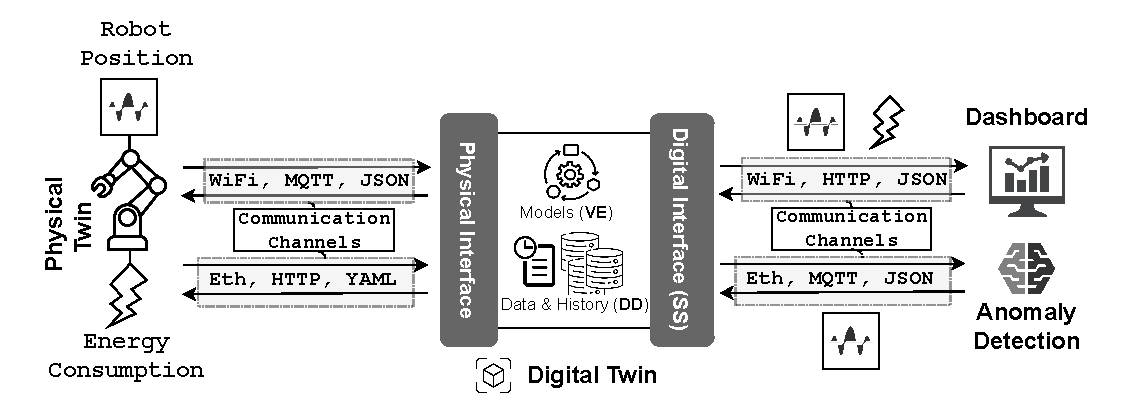
\includegraphics[width=\columnwidth]{figures/dt_application_example.pdf}
    \caption{Example of a DT in an application scenario interacting with a physical asset and digital applications through its PI and DI.}
    \label{fig:dt_application_example}
\end{figure}


Tackling such twofold interoperability challenges requires on one side
the adoption of common data models, semantic interoperability frameworks, and compliance with industry standards~\cite{etsi-dt-comm-requirements-2024} such as OPC-UA\footnote{OPC-UA: \url{https://opcfoundation.org/about/opc-technologies/opc-ua/}}, oneM2M\footnote{oneM2M: \url{https://www.onem2m.org/}}, ISO-23247\footnote{ISO-DigitalTwin: \url{https://www.iso.org/standard/81442.html}}, or the W3C Web of Things\footnote{W3C WoT: \url{https://www.w3.org/WoT/}}.
%
On the other side, the \ac{DT} architecture should accommodate physical and digital heterogeneity \emph{by design} to avoid being locked down in those situations where adherence to a single standard can not be enforced.
Without such measures, \acp{DT} risk becoming fragmented, limiting their ability to collaborate and exchange information across different platforms and applications.
%
The proposal of modular \ac{DT} interfaces aims to address these concerns
at the architectural level, to enhances the interoperability and re-usability of \ac{DT} components in cyber-physical applications.

At an appropriate abstraction level, a \ac{PA} may be digitalized by obtaining and sending data through possibly \emph{several} different \texttt{Communication Channels} (\Cref{fig:dt_application_example}), which 
encompass network protocols, data formats, and physical connections.
The \ac{PI} manages interactions with the \ac{PA}, integrating such channels.
%
Similarly, on the digital side, the \ac{DT} supplies data and insights to applications via the \ac{DI}, adapting to different protocols and representations.

Engineering the \ac{PI} and \ac{DI} requires addressing the challenge of effectively integrating such heterogeneous communication channels.
%
To ensure flexibility and adaptability, it is essential that the core of the \ac{DT}, including its models and implemented behaviors, remains decoupled from the heterogeneous physical and digital communication channels.
%
The \ac{DT}'s shadowing process should focus solely on understanding the available physical data, receiving and transmitting telemetry information, and executing action requests, with no concern for the underlying implementation details.

The remainder of this section describes a proposal for the design the \ac{DT}'s \ac{PI} and \ac{DI}, refining and extending the conceptual model originally proposed in \cite{web-of-dt-ricci-2022} with a concrete implementation based on the concept of modular \emph{adapters}.

%..........................................................
\subsection{Physical Interoperability}
\label{ssec:dte:dt-engineering:physical_interoperability}
%..........................................................

\begin{figure}
    \centering
    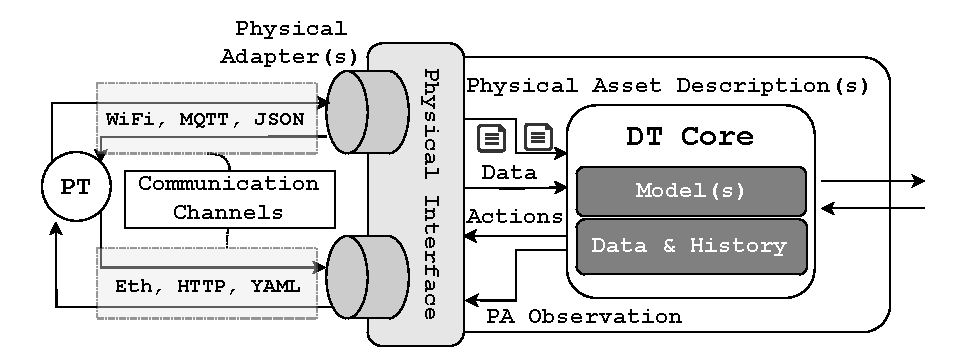
\includegraphics[width=\columnwidth]{figures/dt-interoperability/dt_interoperability_physical.pdf}
    \caption{PI design with modular physical adapters each producing the corresponding \acl{PAD} that is processed by the \ac{DT} Model.}
    \label{fig:physical_interoperability}
\end{figure}


One of the main challenges in facilitating effective communication through the \ac{PI} is the wide variety of communication protocols and data formats used by \acp{PA}.
%
While it can be the case that one \ac{PA} is directly sending all the data concerning its digitalization through only one channel,
it is far more common to build a \ac{DT} aggregating different sources of information~\cite{qi2018dt-and-bigdata}.
%
\ac{IoT} protocols often differ considerably based on the manufacturer, device type, or application domain, making it difficult for the \ac{DT} software to integrate diverse assets.
%
Arguably, the modularity of the \ac{PI}, which encapsulates these responsibilities, is a crucial factor in the design and implementation of interoperable \acp{DT}.
%
Accordingly, the proposal is to design the \ac{PI} as a composition of multiple \emph{\acp{PhA}}: specialized modules capable of interacting with the \ac{PA} using diverse protocols and data formats.
%
As shown in Figure \ref{fig:physical_interoperability}, each \ac{PhA} is responsible for mediating the bidirectional interaction through a single communication channel, simplifying the design and reusability of the component, and making it configurable to adapt to different application contexts.
%
The responsibility of the \ac{PI} becomes then to manage the different \acp{PhA} and make sure the \ac{DT} model can accurately interpret, process, and leverage the data generated by the physical world to create the digital replica and implement its behaviors.
%
Note that although terminology of \ac{PhA} is borrowed from \cite{web-of-dt-ricci-2022}, where it is originally introduced, the \emph{Physical Asset Adapter} proposed in \cite{web-of-dt-ricci-2022} is in fact a conceptual monolithic component, whereas in this concrete proposal a \ac{PhA} is considered as a single-responsibility module of a potentially more complex \ac{PI}.

\subsubsection{Generating \aclp{PAD}}
To facilitate managing different \acp{PhA}, the concept \emph{\ac{PAD}} is introduced: a representation of the capabilities provided by a communication channel in terms of \emph{properties}, \emph{actions}, \emph{events}, and \emph{relationships} that characterize the associated \ac{PA}.
%
Each \ac{PhA}, since it encapsulates the characteristics of a channel, can generate the corresponding \ac{PAD}, effectively decoupling the asset's functionality from the specific communication protocols used.
%
The implementation of the \ac{PAD} generation can be challenging due to the varying capabilities of different communication protocols.
For instance, protocols like \ac{CoAP}~\cite{RFC7252} often come with built-in description and discovery functionalities, which can simplify the process of creating a \ac{PAD} by providing standardized representations of the physical asset's capabilities and behaviors.
On the other hand, protocols like \ac{MQTT}~\cite{MQTTv5} may require developers to add additional information manually to define how information is structured and exchanged, as they do not natively include asset metadata.
In the case of custom or proprietary protocols, the challenge becomes even more pronounced, as these protocols are tailored to specific systems and may lack any standardization or descriptive capabilities.

In all the aforementioned scenarios, the mechanism of \ac{PAD} generation offers a way to encode knowledge about the \ac{PA} bridging the gap by interpreting and extracting relevant information from the protocol used in the associated communication channels.
%
Confining this complexity within the \ac{PI} allows the \ac{DT} model to be agnostic with regard to the complexity of the underlying physical world.

The \ac{PAD} allows the \ac{PI} to discover, extract, and manage asset information and present it to the model that can choose which ones are relevant for the implementation of the \ac{DT} behavior.
%
For example, to create the \ac{DT} of a temperature sensor streaming binary data on MQTT, the \ac{PI} could be composed of a generic MQTT adapter, configured to correctly parse the payload as a decimal number, and generate a \ac{PAD} which advertise the available temperature property to the \ac{DT} model as a Celsius value. 


\subsection{Digital Interoperability}
\label{sec:digital_interoperability}

%%
\begin{figure}[t]
    \centering
    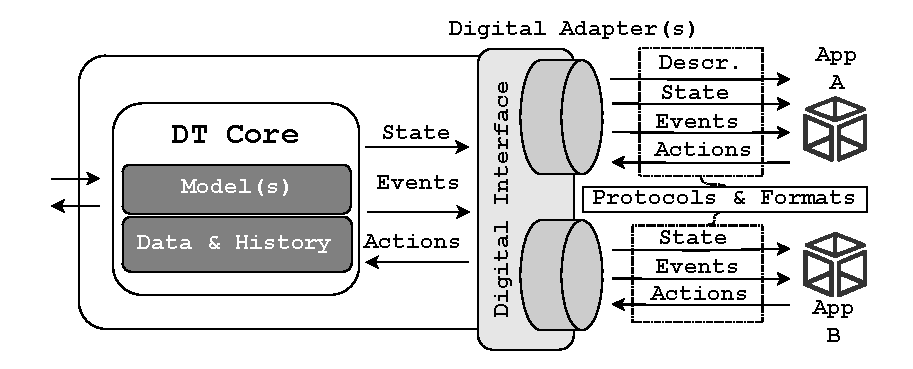
\includegraphics[width=\columnwidth]{figures/dt-interoperability/dt_interoperability_digital.pdf}
    \caption{Digital Interface design with modular adapters and DT description.}
    \label{fig:digital_interoperability}
\end{figure}
%%

As \acp{DT} are meant to bridge between the physical and digital spaces,
interoperability is not only a matter of interfacing with heterogeneous devices, but also other digital applications.
Indeed, despite their initial conception as vertical silos, the concept of \ac{DTE} (\Cref{sec:back:dt:dte}) is emerging to support the the digitalization of complex scenarios through a combination of several \acp{DT}.
%
In this context, \acp{DT} can be used \emph{as-a-service} by other applications implementing the business logic by spanning across different software entities.

To foster interoperability in \acp{DTE}, \acp{DT} must then expose either a standardized general purpose \acf{DI} that can serve different applications or
---following the same design principles adopted to address physical interoperability---
have a modular interface that can satisfy the different needs of different applications
as shown in Figure \ref{fig:digital_interoperability}.

As for \ac{PhA} the terminology is borrowed from \cite{web-of-dt-ricci-2022} and consider to have a \ac{DI} composed of modular \emph{\ac{DiA}}.
The original abstract concept of \ac{DiA} is hence refined to represent a modular component of a more complex \ac{DI}.
Using the concept of \ac{DiA}, the \ac{DI} can expose the \ac{DT} state and services supporting multiple data formats and interaction patterns.
This can be beneficial for integrating it with applications and, especially, legacy systems.
The existence of legacy applications usually implies having little control over the integration requirements, making having more flexible \acp{DT} beneficial to better integrate with the application requirements.

Using several \ac{DiA}, a \ac{DT} could, for instance, support both request-response and publish-subscribe mechanisms to access its current and previous states, support different query languages to access the same data store, expose its current state using different representation formats, etc.
%
This would make the development of the application simpler because adding an application-specific \ac{DiA} won't require intervention in the underlying physical system. 
%
Additionally, the developed application would be more robust and stable since it would depend only on the \ac{DT}, and changes to the physical configuration of the \ac{PA} (e.g., software updates, sensor replacement, network reconfiguration) would have no impact on the application software.
%
Even if the \ac{PA} were to change, (e.g., a software update on a robot changes the telemetry format) the \ac{DI} of the \ac{DT} could stay the same, as the changes would occur within the boundaries of the \ac{PI} and \ac{DT} model.
%
Through this mechanism, \acp{DT} effectively achieve their bridging role, shielding applications from the complexity of physical deployments.

\subsubsection{Describing \aclp{DI}}

A further level of interoperability is possible when allowing \acp{DT} to describe their \ac{DI}, advertising capabilities and available communication channels that applications can exploit.

This is especially relevant in contexts where applications are not bound to a specific interface but can instead process machine-readable descriptions of \acp{DT} and choose to interact with specific assets.
%
A \ac{DT} could then use a \emph{\ac{DTD}}, which, similarly to the \ac{PAD}, can represent the features of the \ac{DT} to its observers.
%
The idea of exposing \acp{DTD} is somewhat present in the major platforms supporting the creation of \acp{DTE}, such as 
Microsoft's \azureTwin{}\footnote{\azureTwin{}: \url{https://azure.microsoft.com/en-us/products/digital-twins}} and \ditto{}\footnote{\ditto{} \url{https://eclipse.dev/ditto/}} and is advocated by standardization activities on interoperability in \acp{DTE}~\cite{etsi-dt-comm-requirements-2024}.

The way such descriptions are implemented may differ significantly, but essentially, they should at least allow representing the \ac{DT}  features and APIs to access them.
%
Notably, differently from the \ac{PAD}, the \ac{DTD} is targeted to external consumers, hence, it should preferably adhere to standard formats and representations to be useful in practice in achieving interoperability.
%
To this end, using Semantic Web technologies (see \Cref{sec:back:web:semantic-web-technologies}) could be a possible solution to implement standard machine-readable \acp{DTD}.
\todo{add forward ref to semantic web descriptors sections}

% \begin{figure*}[t]
%     \setlength{\belowcaptionskip}{-13pt}
%     \centering
%     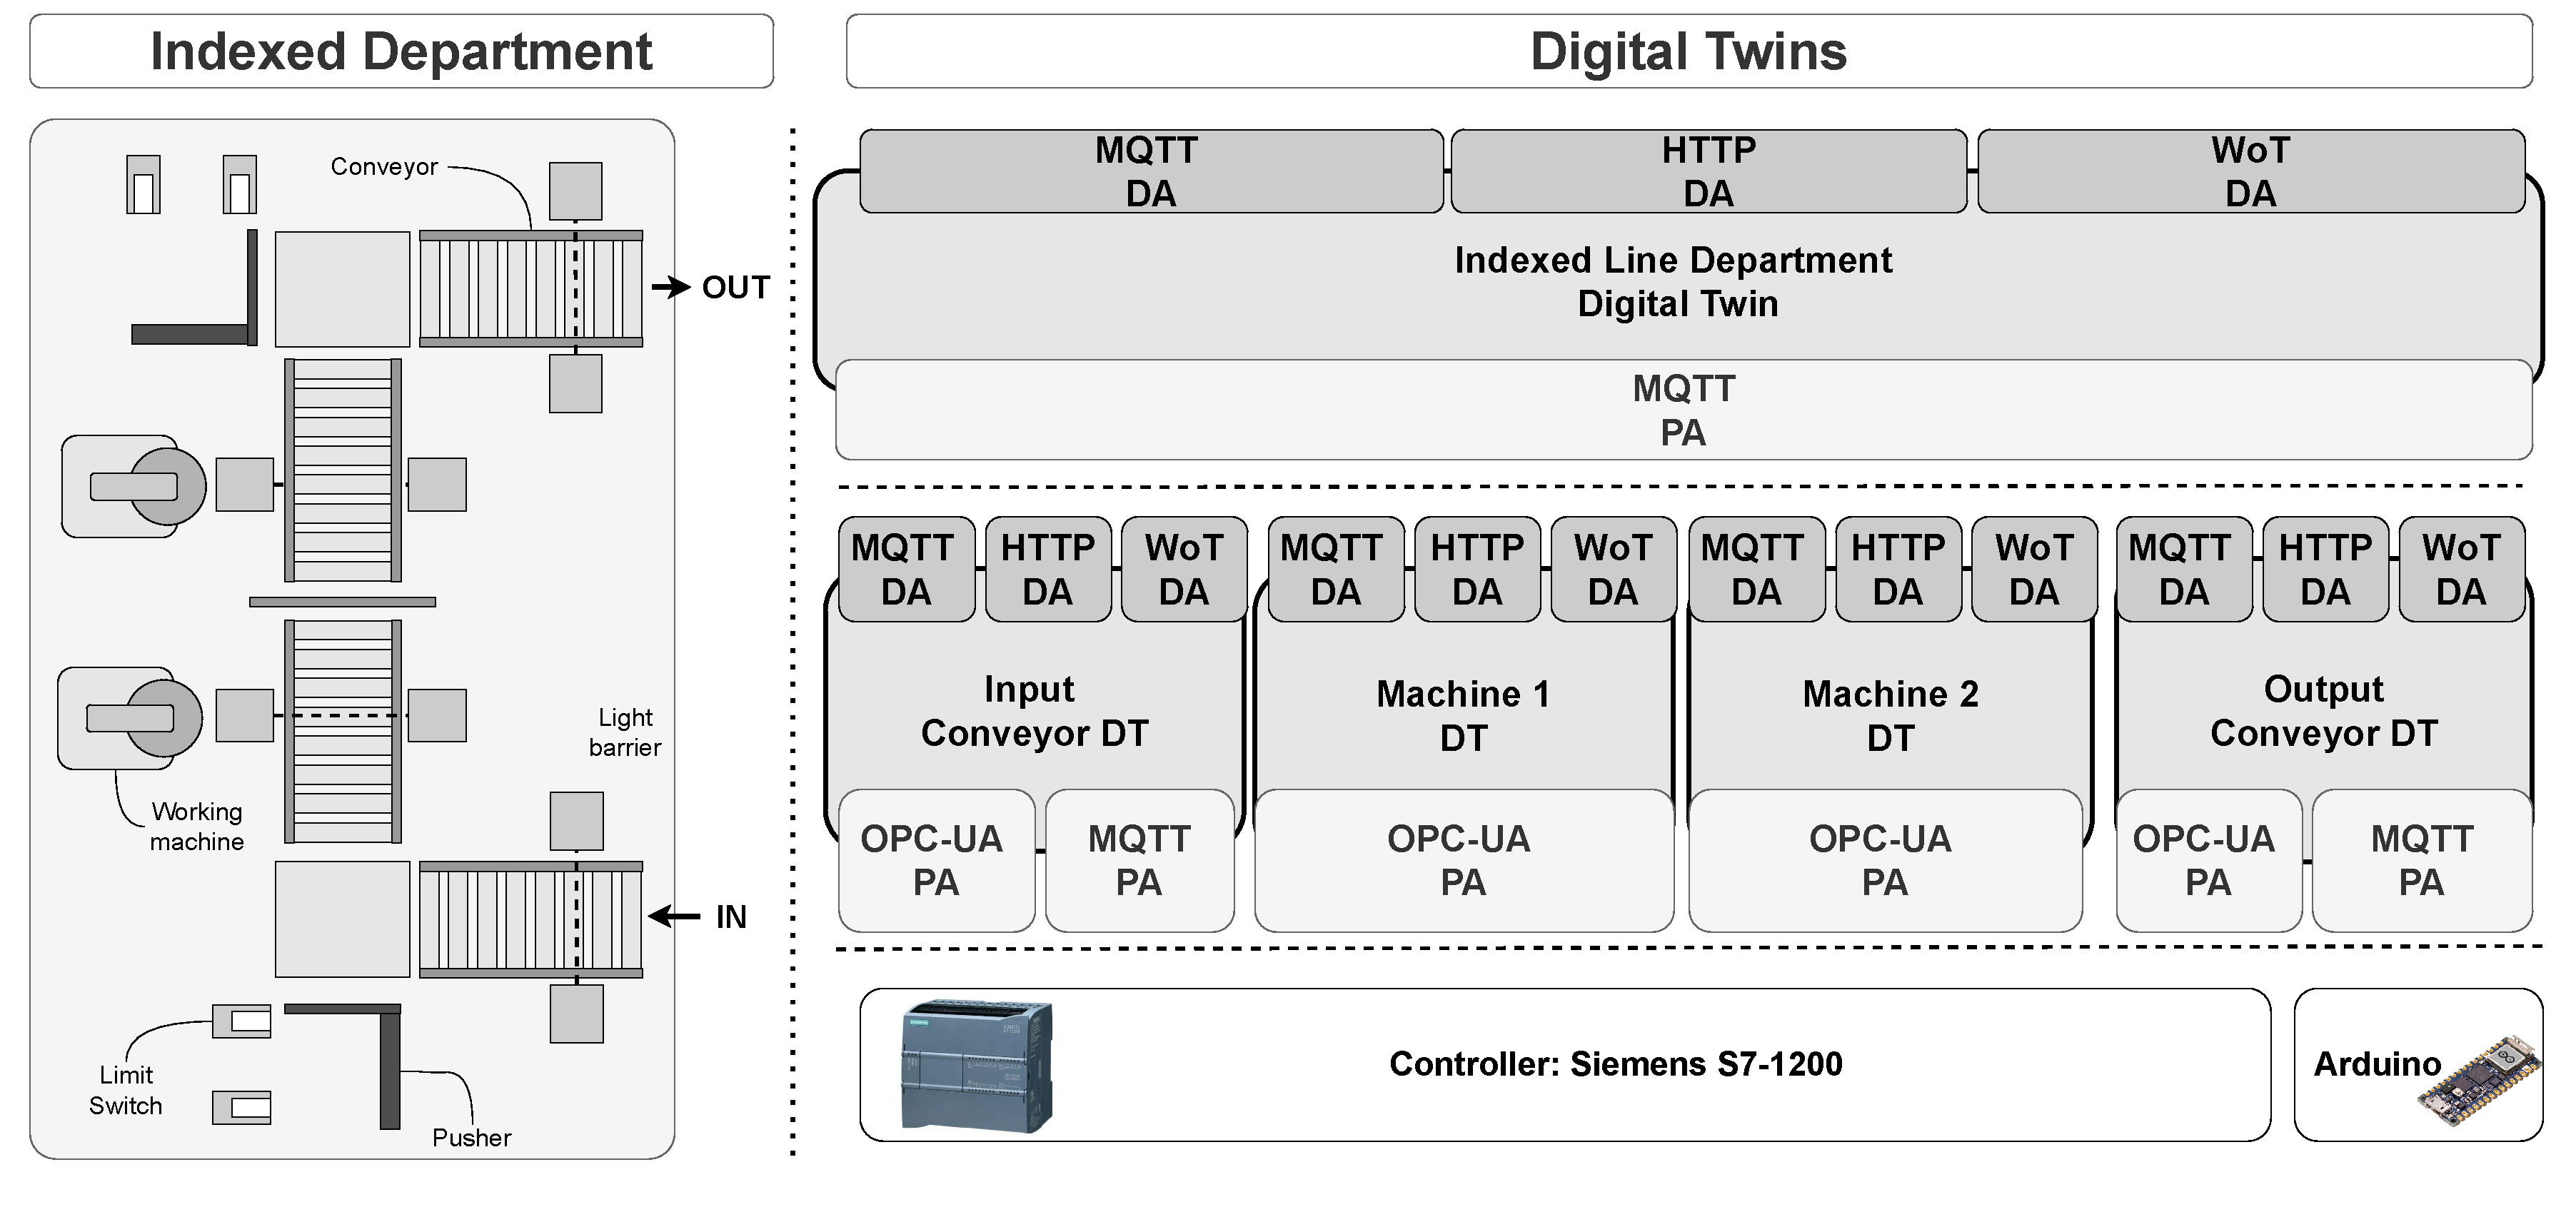
\includegraphics[width=0.93\linewidth]{figures/dt-interoperability/mf_dt_structure.pdf}
%     \caption{The \acl{DT} ecosystem architecture of the microfactory industrial system.}
%     \label{fig:mf_dt_ecosystem}
% \end{figure*}

%-------------------------------------------------------
\subsection{\acl{WoT}: enabling DT Interoperability}
\label{sec:dte:dt-engineering:wot-for-dt}
%-------------------------------------------------------

\ac{WoT}~\cite{wot-arch} standards (\Cref{chap:back:web:WoT}) share the goal of adopting uniform API and data format descriptions to hide low-level complexities and promote interoperability with the proposal of self-descriptive \ac{PhA} and \ac{DiA}.

Despite their similarities, \acp{PAD} and \acp{TD} serve distinct purposes. 
A \ac{TD} provides a structured description of a physical twin's available interactions to external consumers, detailing protocols and interaction possibilities.
%
In contrast, a \ac{PAD} is designed for internal use by the \ac{DT} modules, decoupling the twin's core from the complexities of communication channels.
Its primary role is to facilitate the discovery of available resources and capabilities on the \ac{PA} after establishing a connection with the physical counterpart, providing a structured description of its functionalities and data.
This description is directly interpretable by the \ac{DT} model and independent of the physical characteristics, allowing the reuse of the same model for similar \acp{PA} employing different communication channels.

In contexts in which \ac{WoT} standards are applicable, the devices' \acp{TD} can be automatically mapped to \acp{PAD}, streamlining the \ac{DT} creation process.
Leveraging \ac{WoT} \acp{TD} can significantly reduce the effort required to generate \acp{PAD}, particularly in environments where numerous physical twins already have associated \acp{TD}.
This convergence between \ac{WoT} and \ac{DT} architectures has the potential to accelerate the development and deployment of \ac{DT} solutions by promoting standardization and reusability.
%
Nevertheless, the more general concept of \ac{PAD} can be tailored also to those scenarios in which \ac{WoT} is not applicable. In those cases the responsibility falls back to development (or configuration) of a \ac{PhA} for a specific device to encode the necessary knowledge for the generation of the \ac{PAD}.

\ac{WoT} \acp{TD} can also be used as \acp{DTD}.
The \ac{WoT} architecture actually lists \acp{DT} as one of the possible deployment patterns, with a \ac{DT} mediating the interaction with a \ac{PA} behind a \ac{WoT} interface\footnote{\url{https://www.w3.org/TR/2023/REC-wot-architecture11-20231205/\#digital-twins}}.
%
This is especially useful when devices are not \ac{WoT} compatible or can not be made so due to other constraints, essentially retrofitting the capabilities of the devices with a \ac{WoT} compatible interface.
%
Adhering to \ac{REST} constraints~\cite{fielding2000architectural} and specifically to the HATEOAS and self-descriptive principles, a \ac{TD}-based \ac{DTD} facilitates the discovery of the \ac{DT} model and services.
%
Its machine-readable nature ensures interoperability for applications and consumers.
%
In particular, a \ac{TD}-based \ac{DTD} facilitates the inclusion of \acp{DT} in \ac{WoT} mashups, promoting \acp{DT} as valid \ac{WoT} Things usable by \ac{WoT} Consumers.

Despite its flexibility,
and broad applicability, 
using of \ac{TD} for \acp{DT} presents several limitations in capturing the specific characteristics of \acp{DT} that distinguish them from \emph{Things}.
%
A path to address these limitations could be extending \acp{TD} or supporting additional descriptions specifically for \acp{DT} in \acp{DTE} as explored in \Cref{chap:dte:hwodt}.



%=======================================================
\section{Managing the Digital Twin Lifecycle}
\label{sec:dte:engineering-dt:dt-lifecycle}
%=======================================================


Recently, there has been an increasing recognition of the importance of the lifecycle of \acp{DT},
particularly in distinguishing the properties that define the relationship between the \ac{DT} and \ac{PA}. 
%
Key concepts such as \emph{reflection} and \emph{entanglement} are critical for accurately representing the \ac{PA}~\cite{dt-IoT-context-Minerva-2020,web-of-dt-ricci-2022}.
%
These properties underscore the necessity for a structured lifecycle for the \ac{DT}, ensuring that its state remains consistently aligned with the \ac{PA} throughout various stages.
%
As highlighted in recent surveys~\cite{ferko2022architecting, 9640612,Hribernik_Cabri_Mandreoli_Mentzas_2021}, while the body of literature on \ac{DT} software architectures is growing, most papers are domain-specific and focus on reference models.
%
However, these models often lack concrete guidance on how to implement the internal components of a \ac{DT}. Many of the existing models envision multiple parallel components or models working together, but fail to address how they communicate and interact to maintain consistency in the \ac{DT} state.
This gap leads to potential inconsistencies between the \ac{DT} and \ac{PA}, as the interaction between models and the management of state changes is not adequately captured~\cite{alam2017access,Malakuti2019fourlayer,Lpez2021}.




\begin{figure}[t]
    \centering
    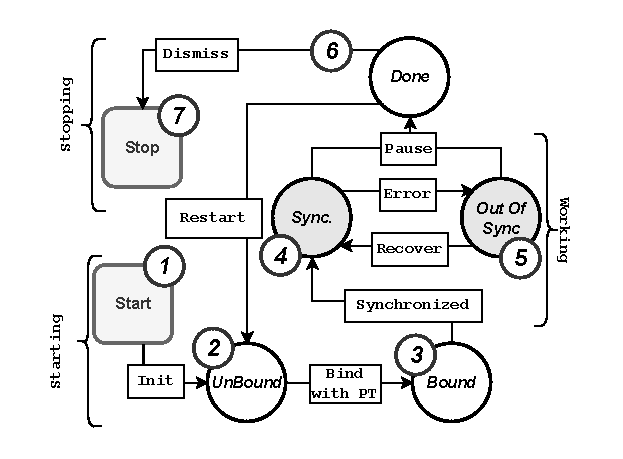
\includegraphics[width=\columnwidth]{figures/wldt_lifecycle_simple.pdf}
    \caption{DT Life Cycle with its phases and transitions.}
    \label{fig:dt_life_cycle}
\end{figure}


%START FROM HERE

%-------------------------------------------------------
\subsection{A Digital Twin Synchronization Lifecycle}
%-------------------------------------------------------

The concept of a \ac{DT} lifecycle has recently been introduced and examined, focusing on its core components and the integration of both the software nature of the \ac{DT} and its ability to synchronize with the \ac{PA} over time~\cite{web-of-dt-ricci-2022}.
%
This lifecycle encompasses the various phases that a \ac{DT} undergoes, as shown in Figure~\ref{fig:dt_life_cycle}, from its creation to deactivation.
%
Since a \ac{DT} is fundamentally a software entity, it is vital to track the evolution of such phases considering the different stages of synchronization with its \ac{PA}.
Proper observation and modeling of this lifecycle are essential to ensure that the \ac{DT} representation can be trusted to reflect the physical counterpart's state consistently when the \ac{DT} is \texttt{Synchronized} and can instead be considered to be outdated in the other phases.

The execution lifecycle of a \ac{DT} can be modeled as follows.
Upon creation (from the \texttt{Started} phase),
the \ac{DT} enters the \texttt{Unbound} phase, where all internal modules are initialized and prepared for the binding process with the \ac{PA}.
%
Once the \ac{DT} successfully binds to its \ac{PA},
meaning the \ac{PA} meets the necessary requirements (expected functionalities and properties)
and the \ac{DT} can communicate with it,
the \ac{DT} enters the \texttt{Bound} phase.
%
During this phase, the \ac{DT} is connected to the \ac{PA} and is ready to begin the shadowing process.

The next phase is the \texttt{Synchronized} phase, 
this is different from simply having established a connection with the \ac{PA}, 
but rather indicates that the \ac{DT} is complying with application-specific requirements
and is receiving the necessary and correct amount of information to be fully aligned with its \ac{PA}.
%
During the synchronization phase the \ac{DT} can compute the \ac{DT} state ($S_{DT}$), ensuring that it is able to accurately reflects the status of its physical counterpart.

If any issues arise, such as network failures, and the \ac{DT} synchronization performance falls under the expected requirements, the \ac{DT} enters the \texttt{Out of Sync} phase.
In this state, the \ac{DT}---while still operational---is unable to update its state reliably. 
%
Eventually, the \ac{DT} may return to the \texttt{Synchronized} phase.

Finally, when the \ac{DT} is no longer required or has completed its function, it transitions to the \texttt{Done} phase.
In this phase, the \ac{DT} remains accessible to external consumers and retains its memory, but it is no longer bound to the \ac{PA} or in sync with it. At the end of the lifecycle, the \ac{DT} can be dismissed and moved to the \texttt{Stopped} phase.
Throughout its lifecycle, the \ac{DT} may also return to the \texttt{Unbound} phase if errors are detected during the binding process or if it is rebooted or restarted.


%-------------------------------------------------------
\subsection{Binding the DT with the PA}
%-------------------------------------------------------

The transition from the Unbound to Bound phase in the \ac{DT} lifecycle remains an open research area:
a key challenge is identifying whether all the capabilities of the \ac{PA} relevant to support the \ac{DT}'s behavior are available so that the shadowing process can start.

The modular design of the \ac{PI} presented in the previous section (\Cref{ssec:dte:dt-engineering:physical_interoperability}) can have support this transition.
%
Namely, once a \ac{PhA} successfully connects to the \ac{PA}'s channel and starts receiving data from it, it can send the generated \ac{PAD} to the \ac{DT} model.
The generation of the \ac{PAD} can be used as a synchronization step to signify that the \ac{PhA} is successfully connected to the \ac{PA}.
%
The \ac{DT} model is then responsible for collecting the different \acp{PAD}, assessing whether all the relevant information to start computing the \ac{DT} state is available and consequently moving on to the \texttt{Bound} phase.
%
This mechanism enables managing the \ac{DT} behavior consistently, even with the additional complexity of the modular \ac{PI} design.

Of course the challenge still stands in managing each individual \ac{PhA} connection, but this decoupling through \acp{PAD} allows \ac{DT} developers to establish functional binding requirements that are independent of technical details. 

%--------------------------------------------------------
\subsection{Managing DT and PA Synchronization}
%--------------------------------------------------------


The most significant challenge in current \ac{DT} lifecycle modeling is the broad characterization of the \texttt{Synchronized} phase, which
only generically considers synchronization requirements between the \ac{PA} and the \ac{DT}, without having explicit awareness of the \ac{PA} lifecycle and the potential changes in its operational context.
This general and unstructured approach limits the ability to model the lifecycle in a consistent and uniform manner, failing to properly address the dynamism of the \ac{PA} behavior.

The \texttt{Synchronized} phase of the \ac{DT}'s lifecycle assumes a continuous exchange of information between the \ac{DT} and its associated \ac{PA} usually measured to maintain a frequency within a given threshold, to guarantee that information on the \ac{DT} is \emph{fresh} and can hence be trusted as a valid representation of the \ac{PA} state. 

However, this general assumption may not always hold true due to variations in the \ac{PA}'s internal states.
% The issue arises because \ac{PA} can adjust telemetry frequency and have different value ranges over time, depending on the phases of their lifecycle and their operational context (e.g., from \texttt{Ready} to \texttt{Working}).
% These variations introduce complexity in maintaining the cyber-physical alignment. 
% Without appropriate modeling, these changes might be misinterpreted as failures while they are instead expected variations due to the \ac{PA}'s phase transition.
%
In some cases, \acp{PA} can enter operational states that temporarily inhibit their ability to communicate, even while maintaining an active connection to the \ac{DT}.
These are scenarios in which the absence of messages from the \ac{PA} does not necessarily indicate a failure or misalignment but rather reflects the \ac{PA}'s operational context.
For instance, a \ac{PA} might enter a \texttt{Rebooting} state during which it cannot send telemetry data.
Similarly, resource constraints on the \ac{PA}, such as \textit{CPU overload} or \textit{network bandwidth exhaustion}, may result in disrupted or paused communication that may or may not be tolerable for the \ac{DT} model and application.
%
In other cases, the \ac{PA} may not entirely cease communication but instead alter its update frequency in response to operational changes. For example, an industrial robotic arm might increase its data transmission frequency during a high-precision assembly task to provide real-time feedback, while it could reduce the update rate to conserve energy and network bandwidth when in an idle or maintenance mode.


\begin{figure}
    \centering
    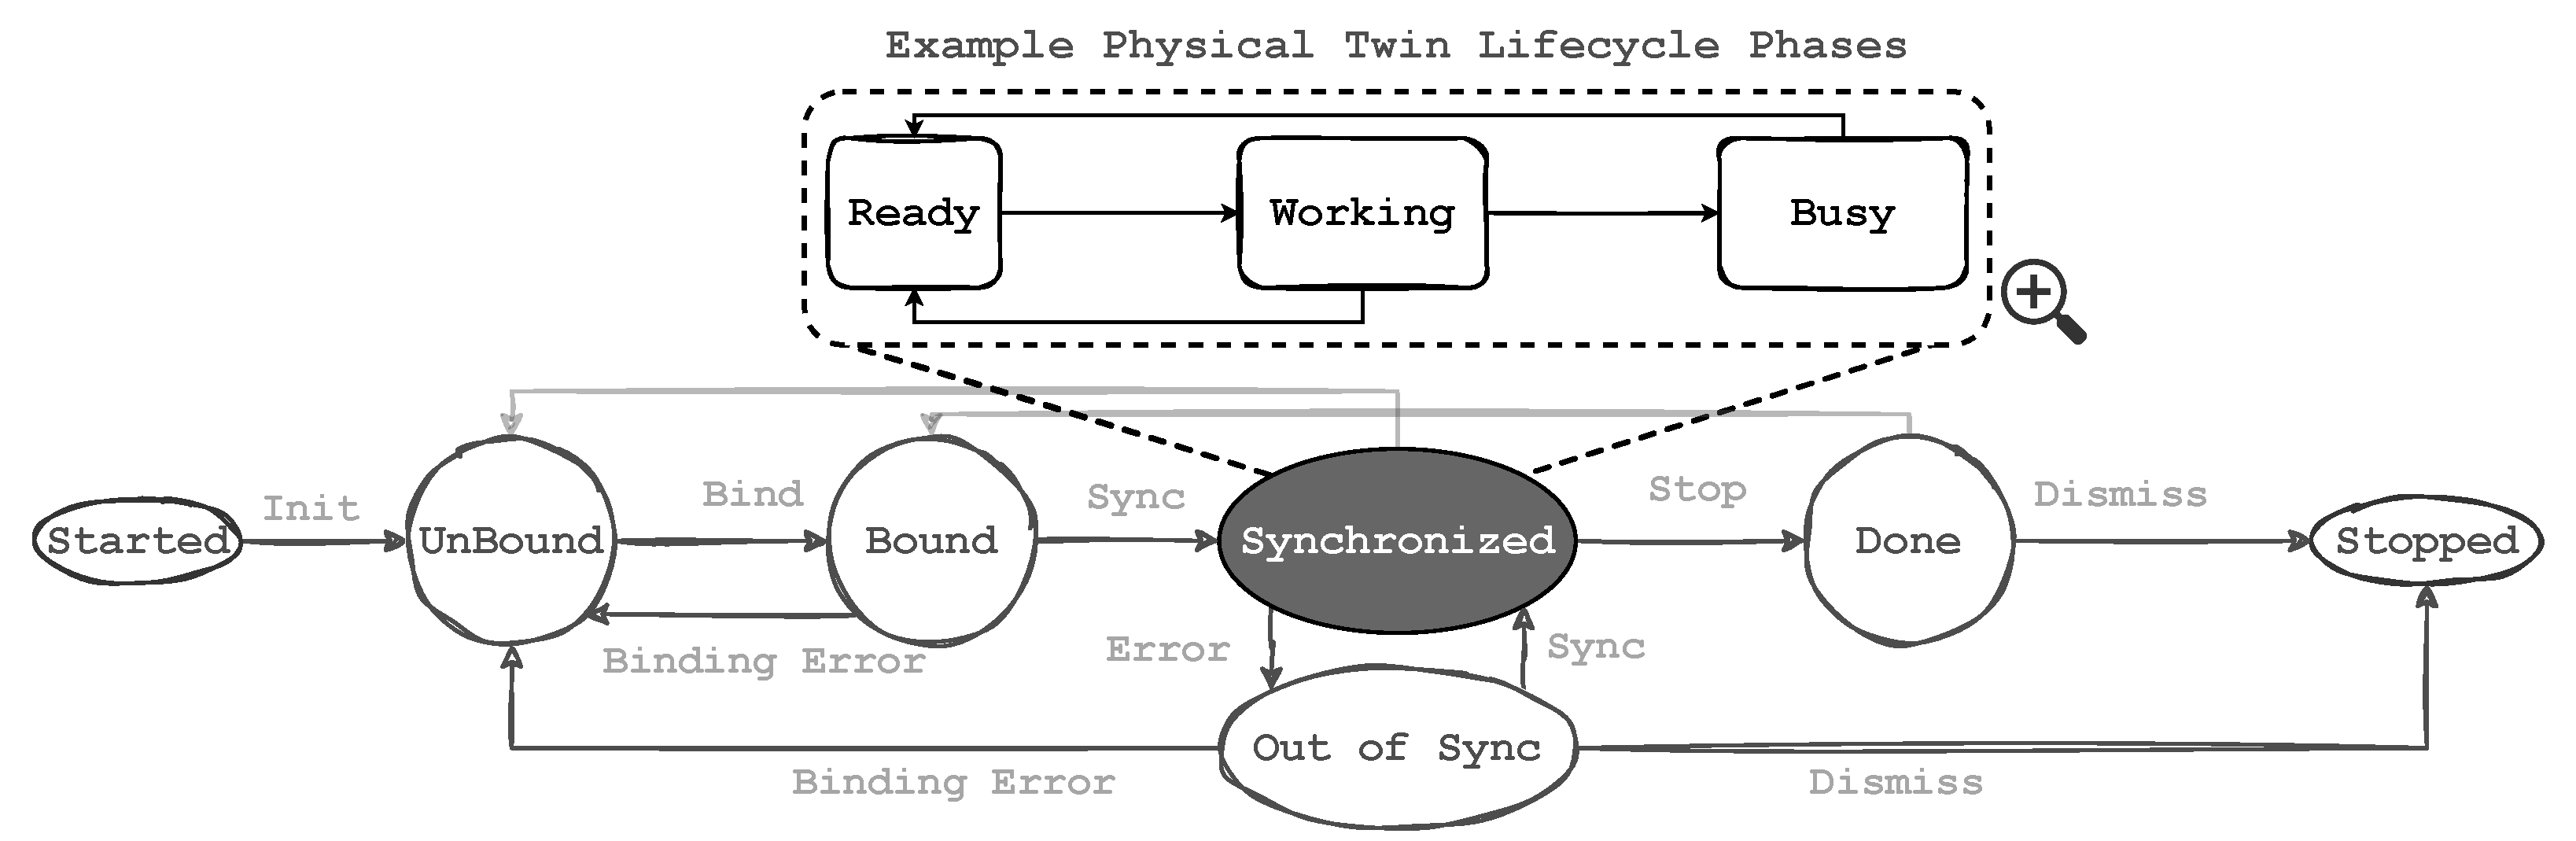
\includegraphics[width=\textwidth]{figures/dt-lifecycle/dt_lifecycle_pt_sync.pdf}
    \caption{Schematic representation of the \ac{DT} lifecycle with a structured example of the Synchronized phase.}
    \label{fig:dt_lifecycle_pt_sync}
\end{figure}


This adaptive behavior necessitates that the \ac{DT} \emph{dynamically adjust its expectations} and processing strategies based on the \ac{PA}'s operational state, avoiding false-positive anomalies caused by \emph{intentional} communication variability.  
By distinguishing between inhibited communication (e.g., \texttt{Rebooting} or \texttt{Overloaded}) and adjusted communication patterns (e.g., frequency scaling in \texttt{Idle} vs. \texttt{Active} states), the \ac{DT} can better align with the \ac{PA}'s lifecycle.
This alignment ensures the \ac{DT} remains a reliable digital counterpart, accurately reflecting the \ac{PA}'s operational context and providing a robust foundation for decision-making.  

To address these situations, the \ac{DT} must incorporate mechanisms to: 
\begin{itemize}
    \item \emph{Detect and Classify Non-Communication States:} Recognize when the lack of communication from the \ac{PA} is due to a valid operational state (e.g., rebooting) rather than a system failure;
    \item \emph{Model \ac{PA} State-Dependent Communication Behavior:} Explicitly account for \ac{PA} states that imply non-communication, such as \textit{idle}, \textit{rebooting}, or \textit{overloaded}, within the lifecycle framework. 
\end{itemize}
This requires extending the \ac{DT} lifecycle model (\Cref{fig:dt_life_cycle}) to represent such scenarios accurately.


The proposal is to refine the \texttt{Synchronized} phase by introducing sub-phases that correspond to the \ac{PA}'s operational states (\Cref{fig:dt_lifecycle_pt_sync}).
For example, in the industrial domain, a \ac{DT} of a machine may enter the \texttt{Synchronized} phase but should then transition through more specific sub-phases such as \texttt{Ready}, \texttt{Working}, or \texttt{Busy}.
Each of these sub-phases would have clearly defined transition criteria, phases, and associated $S_{\ac{DT}}$, providing a more granular and accurate representation of the \ac{DT}'s behavior.

To formalize this approach, the overall \ac{DT} lifecycle phase at a given time $t$ $LP_{DT}(t)$ can be defined as a composition of the \ac{PA} lifecycle phase $LP_{PA}(t)$ and the \ac{DT} software lifecycle phase $LP_{Soft.}(t)$, as shown in Eq.~\ref{eq:lpdt_definition}.

\begin{equation}
LP_{DT}(t) = \langle  LP_{PA}(t), LP_{Soft.}(t)\rangle
\label{eq:lpdt_definition}
\end{equation}

The \ac{DT} representation of the asset $R_{DT}$ can hence be characterized at any given time instant $t_i$ by its lifecycle phase $LP_{DT}(t_i)$, its current state $S_{DT}(t_i)$, and its history $H(t_a, t_b)$ over a specific time interval $(t_a, t_b)$, as shown in Eq.~\ref{eq:dt-definition}.

\begin{equation}
R_{DT}(t_i) = \langle LP_{DT}(t_i), S_{DT}(t_i), H(t_a, t_b)\rangle \quad \text{and} \quad  t_a, t_b \leq t_i
\label{eq:dt-definition}
\end{equation}

The values of the different components of the \ac{DT} at the time instant $t_i$ can then be mapped as a function of the different possible values of $LP_{Soft.}$, as detailed in Eq.~\ref{eq:lpdt_complete_mapping}.

\begin{equation}
\begin{split}
R_{DT}(t_i) = {} &
\begin{cases}
    LP_{PA} = \emptyset, \ S_{DT} = \emptyset, \ H = \emptyset,\\
    \quad \text{if } LP_{Soft.} \in \{\texttt{Started}, \texttt{Stopped}\}, \\[0.4em]
    LP_{PA} = \emptyset, \ S_{DT} = \emptyset, \ H = H(t_f, t_o),\\
    \quad \text{if } LP_{Soft.} \in \{\texttt{UnBound}, \texttt{Bound}, \texttt{OutOfSync}\}, \\[0.4em]
    LP_{PA} = LP_{PA}(t_i), \ S_{DT} = S_{DT}(t_i), \ H = H(t_f, t_i),\\
    \quad \text{if } LP_{Soft.} = \texttt{Synchronized},\\[0.4em]
    LP_{PA} = \emptyset, \ S_{DT} = \emptyset, \ H = H(t_f, t_d),\\
    \quad \text{if } LP_{Soft.} = \texttt{Done}
\end{cases}
\end{split}
\label{eq:lpdt_complete_mapping}
\end{equation}

When $LP_{Soft.}$ is \texttt{Started}, it represents the initialization phase where the \ac{DT} software has been instantiated. At this stage, $LP_{PA}$ is undefined since no communication with the \ac{PA} has been established. 
Similarly, $S_{DT}$ has not been computed, as the \ac{DT} has not acquired any state information. The history $H$ is also empty, as no synchronization or state updates have occurred yet.

When $LP_{Soft.}$ is \texttt{Unbound}, it indicates that the \ac{DT} is operational but not yet synchronized.
In this phase, $LP_{PA}$ remains undefined because the \ac{PA} lifecycle phase cannot be detected.
$S_{\ac{DT}}$ is also undefined since the \ac{DT} can not compute the state yet.
However, the history $H$ retains information about events recorded from the first connection data received from the \ac{PA} $t_{f}$ to the moment the \ac{DT} transitioned out of the synchronized phase, marked by $t_{o}$.
%
The same happens when the \ac{DT} is \texttt{Bound}, as the state has not been computed yet, 
or if the \ac{DT} is \texttt{Out of Sync}, as the state can no longer be updated.

When $LP_{Soft.}$  is \texttt{Synchronized}, the \ac{DT} is fully synchronized with the \ac{PA}.
In this state, $LP_{PA}$ corresponds to the lifecycle phase of the PA (e.g., in the example of Fig.~\ref{fig:dt_lifecycle_pt_sync}, this could be the \texttt{Working} phase) at the time $t_i$.
At this point, $S_{DT}$ contains the current computed state of the \ac{DT}, reflecting the alignment between the \ac{DT} and \ac{PA}.
The history $H$ encompasses all events and states up to the current time $t_{i}$, documenting the \ac{DT}'s evolution in sync with the PA.
If the \ac{DT} operates correctly, it can remain in the \textit{Synchronized} phase for the duration of its lifecycle, continually updating as the PA's lifecycle progresses.
During this phase, multiple records of lifecycle evolution can be captured as $LP_{PA}$ evolves (e.g., moving from \texttt{Working} to \texttt{Busy}), and multiple computations of $S_{DT}$ may occur within the same $LP_{PA}$.
For instance, while in the \texttt{Working} phase, the \ac{DT} could compute multiple states corresponding to variations in physical properties such as accelerometer readings or energy consumption, ensuring the \ac{DT} continuously reflects the PA's behavior in a dynamic and precise manner.

When $LP_{Soft.}$ is \texttt{Done}, the \ac{DT} synchronization has been intentionally paused, and the \ac{DT} remains active for accessing stored information. In this phase, $\text{LP}_{PA}$ is empty, $S_{DT}$ is empty, and $H$ contains the history until the time the \ac{DT} is decommissioned denoted as $t_{d}$.

Finally, when $LP_{Soft.}$ is \texttt{Stopped}, the \ac{DT} lifecycle is terminated. $LP_{PA}$ is empty, $S_{DT}$ is empty, and $H$ is also empty, as the \ac{DT} is offline and data is no longer accessible.

By clearly defining and distinguishing between the various phases, the approach enhances the alignment between \ac{DT}s and their physical counterparts, ensuring that each transition and state change is accurately captured and reflected.
The main benefits of this approach include: 
\begin{itemize}
    \item \textit{Enhanced Cyber-Physical Awareness}: a structured lifecycle model ensures that critical transitions of phases and states of the \ac{PA} are precisely tracked and understood, enhancing the overall awareness and responsiveness of the system;
    \item \textit{Better Decision-Making}: with a clear understanding of each phase and its impact, applications and services can make more informed decisions based on accurate and timely information about the current relationship between \ac{PA} and \ac{DT};
    \item \textit{Adaptability}: this structured approach can be adapted to various applications, making it versatile and applicable across different domains.
\end{itemize}

The approach assumes that the $L_{PA}$ is either provided by the \ac{PA} or can be identified by the \ac{DT} model (e.g., through a classification model).
Modeling these phases can be challenging, especially for complex \acp{DT}.
Despite improved cyber-physical awareness, phases may still be incorrectly mapped due to unforeseen external factors.
Additionally, phase tolerance could impact anomaly detection within the DT, necessitating methodological trade-offs to set this tolerance correctly.

Despite these open challenges, the proposed structured lifecycle model represents an advancement in managing \ac{DT} synchronization with their physical counterparts, providing a robust foundation for future developments.

%=======================================================
\section{Modeling Augmentation Functionalities}
\label{sec:dte:engineering-dt:dt-augmentation}
%=======================================================

\acp{PA} are typically limited by the nature of their physical characteristics throughout their lifecycle. In contrast, \acp{DT} can capitalize on software-based flexibility to modify, update, and enhance functionality over time.
These enhancements are accessible through \ac{DT} \acp{API} and can be powered by data-driven models possibly enabling adaptive and intelligent behaviors.
This core property of \acp{DT} is known as \emph{augmentation}~\cite{dt-IoT-context-Minerva-2020}.

Examples of DT-enabled augmentation include adding technical features to retrofit devices through external software, such as enhancing interoperability of \ac{IoT} devices via protocol and data format translation. Another example involves improving security and addressing unresolved bugs by mediating interactions with outdated devices that no longer receive updates. Additionally, \acp{DT} can enhance device services by introducing new high-level actions for operations, or by implementing advanced functionalities powered by machine learning and \ac{AI} algorithms, such as forecasting, anomaly detection, and pattern recognition (\Cref{sec:back:dt:ai}).

Despite the acknowledgment of augmentation as a defining feature of \acp{DT},
this property is often defined only conceptually, with implementations tailored to specific vertical cases.
The lack of a reference model for defining \ac{DT} augmentation results in unclear design patterns and potential performance limitations.
Indeed, without a well-defined and measurable boundary for augmentation features---including resource allocation---the \ac{DT} risks failing to achieve its design goal of accurately representing the \ac{PA} with sufficient \emph{fidelity}~\cite{Bellavista_Bicocchi_Fogli_Giannelli_Mamei_Picone_2023}.

%--------------------------------------------
\subsection{Extending the DT Model with Augmentation}
%--------------------------------------------

The \ac{DT} model introduced in \Cref{sec:dte:engineering-dt:abstract-architecture} is here extended to explicitly include augmentation functionalities.
%
In practical terms, augmentation serves as a bridge transforming raw data into meaningful, actionable outcomes guided by the underlying model.
\acp{DT} may expose additional services and functionalities that enhance the capabilities of the \ac{PA}.
Such functionalities can be represented as a set of \emph{augmentation functions} $F$, where $Augm_{i}$ denotes the individual augmentation functions implemented within the DT. Each augmentation function $Augm_i$ may leverage a specific model $m \in M$, to interpret and respond to changes in the DT.

\begin{equation}\label{eq:augm_set}
    F = \{Augm_{1}, Augm_{2}, \dots, Augm_{n}\}\\
\end{equation}

The model in \Cref{eq:5D_dt_model} can hence be extended to: 

\begin{equation}
DT = \langle PI, M, Shad, F, H, DI \rangle
\tag{\ref{eq:5D_dt_model}}
\end{equation}

Augmentation functions can be distinguished based on two aspects:


\paragraph{Triggering mechanism} (\( \tau \)): defines how and when the function is activated in response to events within the \ac{DT}.
%
\begin{equation}
\tau \in \{ e_{DT}, e_{Aug}, e_{Time} \}  \sigma \in \{S_{aug}, \varnothing\}
\end{equation}
%
\(\tau\) can be an event of three types:
%
\begin{itemize}
\item \( e_{DT} \) represents the output from the shadowing process indicating a new computation of the \ac{DT} state \( S_{DT} \);
\item \( e_{Aug} \) can be generated either as the output of another augmentation function or as a direct invocation by the shadowing process;
\item \( e_{Time} \) refers to temporal triggers and can be used to model periodic execution or specific scheduled tasks.
\end{itemize}
%
Notably, augmentation functions can not respond to triggers coming directly from the \ac{PI} as such $e_{PA}$.
Physical events need to be processed by the shadowing process first, which may in turn select the activation of a relevant augmentation function firing a specific $e_{Aug}$.



\paragraph{State management} (\( \sigma \)): indicates whether the function maintains an internal state that persists over time or is \emph{stateless}.
%
\begin{equation}
\sigma \in \{S_{aug}, \varnothing\}
\end{equation}
%
A stateful function possesses a state \( S_{Aug} \) that evolves and persists over time in alignment with the evolution of the \ac{DT}.  
A stateless function simply reacts to triggers without maintaining any memory of previous invocations.  
Notably, modeling stateful functions allows for the representation of processes that may even run in parallel with the \ac{DT} main control flow, producing new events \( e_{Aug} \) asynchronously.  
Since the function is stateful, it is triggered to start but can persist over time, as its execution is fully encapsulated within the function context. Additionally, the function may receive new triggers over time that feed into its ongoing process.

The output of an augmentation function \( Augm_{i} \) is determined by its inputs and can be expressed as:

\begin{equation}
    Augm_{i}(\tau, m, \sigma, H) =
    \begin{cases}
    e_{Aug} & \text{\textbf{if} $m$ matches}\\
    \varnothing & \text{\textbf{otherwise}}
    \end{cases}
\end{equation}

The triggering event $\tau$ may carry important information for the function execution.
The parameter $m \in M$ represents the model used within the augmentation function, encapsulating the rules, logic, and conditions that define how the function interprets its inputs and determines the output.
The model is crucial for evaluating whether the function should generate an output based on the current state of the function $\sigma$ and context, which is represented by the \ac{DT} history $H$ which includes the latest state $S_{DT}$.

The output \( e_{Aug} \) represents an event generated by the augmentation function, signaling that the conditions defined by the model \( m \) have been met. Conversely, if the conditions are not satisfied (i.e., if \( m \) does not align with the current state or inputs), the output will be \( \varnothing \), indicating that no new event has been produced.  
This approach captures the idea that the execution of an augmentation function does not always result in the generation of a new event. For example, in the case of an anomaly detection model, an event is only triggered when an anomaly is detected with a certain confidence threshold, meaning that no event is generated if the conditions for an anomaly are not met.
Since $e_{Aug} \in \tau$, augmentation functions can also be chained to model processing pipelines triggered by the outputs of previous functions.

%--------------------------------------------
\subsection{Impact on Shadowing}
%--------------------------------------------

The introduction of augmentation functions requires to adapt the shadowing process to handle augmentation events. Indeed, the shadowing process should be capable of receiving relevant augmentation events (e.g., detected anomalies) and use them to update the state of the DT, as illustrated below:

\begin{equation}
    e_{DT}(S_{DT}) = Shad_{DT \rightarrow DT}(M, e_{Aug}, H)
\end{equation}

The same principle applies when a physical event triggers an augmentation function. There is no direct link between physical world events (\( e_{PA} \)) and augmentation functions; 
instead, the decision to trigger an augmentation function based on the receipt of a physical event is mediated by the shadowing process.
The shadowing process analyzes the \( e_{PA} \) and determines whether it is relevant for an augmentation function in $F$ (or multiple functions simultaneously).  If the event is deemed as relevant, the shadowing process generates a trigger by producing an augmentation event (\( e_{Aug} \)), which then serves as the trigger \( \tau \) for one or more augmentation functions.

\begin{equation}
    e_{Aug} = Shad_{PA \rightarrow DT}(M, e_{PA}, H, F)
\end{equation}


Similarly, actions requests that are received by the \ac{DT} ($a_{DT}$) can also trigger augmentation functions.
Again, there is no direct relationship between the action taken on the DT, as represented by its state, and the execution of the augmentation function. Instead, this process also goes through the shadowing process, which matches the request received on the \ac{DI} with the corresponding augmentation function trigger, thus generating an augmentation event that will serve as the trigger for the augmentation function.
This can be used to model a request-response pattern for the execution of augmentation functions such as requesting the predicted next state of the \ac{DT}. In such cases, since the result of the augmentation does not impact the state of the \ac{DT}, the result can be directly routed to the external consumer of the \ac{DT}.

\begin{equation}
    e_{Aug} = Shad_{DT \rightarrow DT}(M, a_{DT}, H, F)
\end{equation}


Despite the shadowing might not be required to validate the result of an augmentation function triggered by an action request, it is still enforced to handle the incoming requests. 
This design aims to decouple the available implementations of the augmentation functions from the actions presented on \ac{DI} and handle this transparently from the consumer perspective.
For example, there might be several augmentation functions implementing a given functionality and it would be up to the shadowing process to determine which one is best suited to respond to a specific request depending on the current context of the \ac{DT} (e.g. the state prediction functionality could be implemented using different specialized models depending on some conditions in the state of the \ac{DT}).

%----------------------------------------------
\subsection{Engineering Augmentation Functions}
%----------------------------------------------

Engineering augmentation functions following the proposed model requires defining
software architectural patterns that can be practically applied to implement them.
Depending on the implementation, it is possible to define \emph{internal} and \emph{external} augmentation.  
This setup allows for the dynamic addition of new functionalities to the \ac{DT}, either through external or internal processing.

\begin{figure}
    \centering
    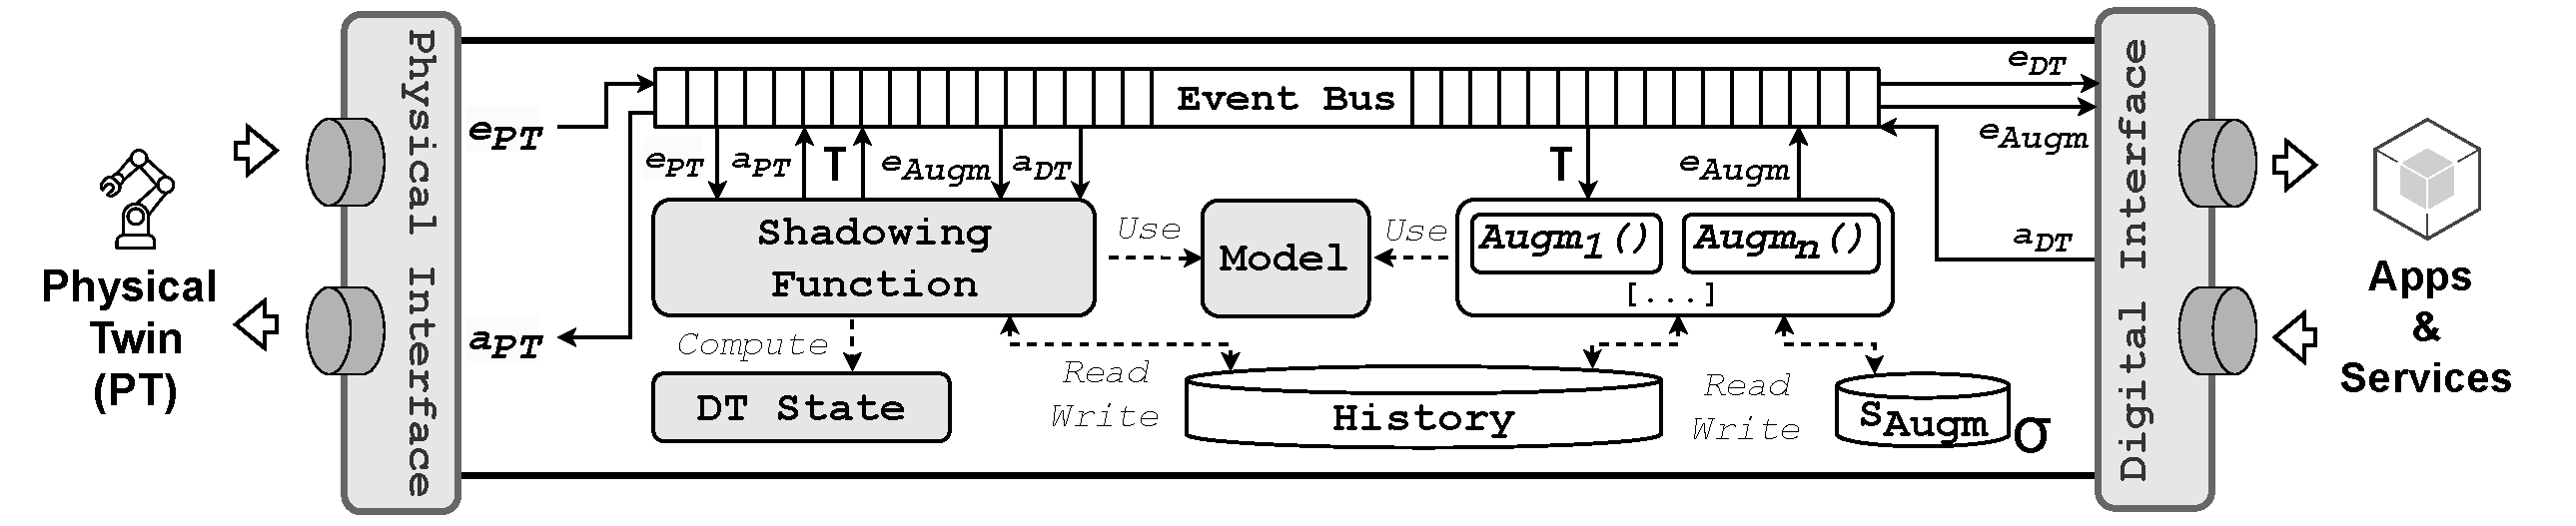
\includegraphics[width=\textwidth]{figures/event_driven_augmentation.pdf}
    \caption{Event-Driven architecture of a DT to support and enable effective Augmentation function management and execution.}
    \label{fig:event_driven_augmentation}
\end{figure}

As \Cref{fig:event_driven_augmentation} shows, the core architecture of the \ac{DT} is centered around a shared \texttt{Event Bus}, which serves as the communication backbone, handling events and actions within the \ac{DT} system.
Starting from the \ac{PI}, physical events \( e_{PA} \) are processed by the \texttt{Shadowing Function} ($Shad$) which computes the \ac{DT} State $S_{DT}$ based on the received events and the \texttt{\ac{DT} Models} ($M$), ensuring that the \ac{DT} accurately reflects the current state of the \ac{PA}.
The \texttt{\ac{DT} State} component maintains this state in memory, while the \texttt{History} ($H$) component persists past events and states for reference and analysis.

\texttt{Augmentation Functions} (\( Augm_{i} \)) provide additional capabilities or insights to the \ac{DT}, interacting with \( M \), \( H \), and internal state information \( \sigma \).
The interaction between the \( Shad \) and the \( Augm_{i} \) is entirely event-driven, based on trigger events \( \tau \) and \( e_{Augm} \) flowing out of the augmentation functions with their results.
These results are then sent to the \( Shad \) for further state computation and to the \texttt{Digital Interface} (\( DI \)) to respond to requests for \( Augm_{i} \) from external services and applications.
The \( DI \), mirroring the \ac{PI}, handles outgoing events of the \ac{DT} (e.g., \( e_{DT} \) carrying the new \( S_{DT} \) or its variations) or \( e_{Augm} \) with the results of an augmentation function, and manages incoming actions and requests from digital entities as digital actions \( a_{DT} \).

\begin{figure}
    \centering
    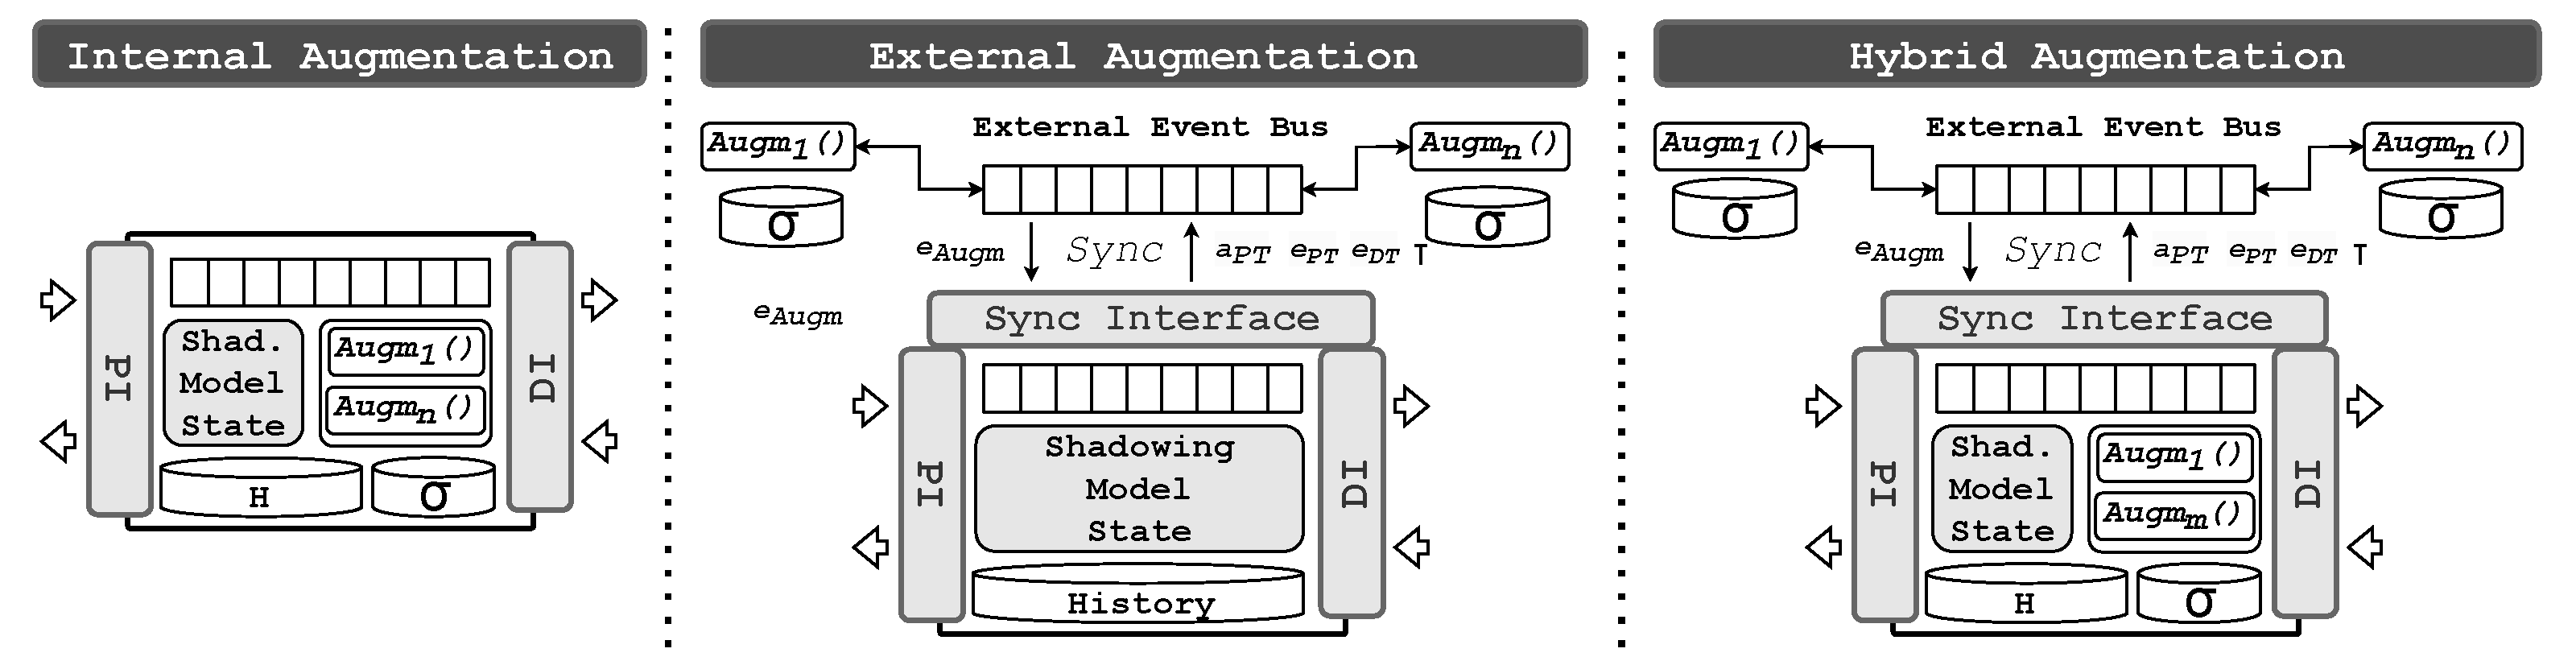
\includegraphics[width=\textwidth]{figures/augmentation_patterns.pdf}
    \caption{Patterns for augmentation functions execution: internally (left), externally (center), or through a hybrid solution (right).}
    \label{fig:augm_function_event_driven_patterns}
\end{figure}


Based on this event-driven model, it is possible to identify three approaches for implementing augmentation functions (\Cref{fig:augm_function_event_driven_patterns}):
\begin{itemize}
    \item \textit{internal} augmentation, where functions are executed within the \ac{DT} process;
    \item \textit{external} augmentation, where functions are executed outside the \ac{DT} process by means of an external service;
    \item \textit{hybrid} augmentation, where functions are executed through a combination of internal and external processes.
\end{itemize}

\subsubsection{Internal Augmentation}
Augmentation functions are executed \textit{internally}, i.e. within the same operating system process as the \ac{DT}, thus sharing the same resources allocated to the \ac{DT} instance (e.g., CPU or GPU computation capabilities).
From an external perspective, these functions are perceived as internal functionalities of the \ac{DT} and only the internal event bus of the \ac{DT} is used.

This approach ensures low latency and tight integration with the \ac{DT} core functionalities, as overhead between the \ac{DT} and the augmentation functions is minimized.
%
For instance, in a manufacturing scenario an internal augmentation function could periodically monitor the operational parameters of a machine physical counterpart.
By running within the \ac{DT} process, this function can quickly react to changes in the machine state, such as detecting abnormal vibrations that might indicate a potential failure (e.g., using signal processing approaches).
The internal event bus would handle the real-time data stream from the machine sensors, feeding the computation of the \ac{DT} state while allowing the augmentation function to promptly process this data and update the \ac{DT}.

\subsubsection{External Augmentation}
Augmentation functions run \textit{externally} as processes entirely separate from the \ac{DT}, possibly without any knowledge of the \ac{DT} internal model.
Since the functions are implemented on external processes, they can use inter-process communication to synchronize and hence they can be distributed across different computing nodes and resources, for a more fine-grained allocation.
%
This translates either in multi-process deployment of the \ac{DT} on the same host, or possibly in fully distributed deployment of the \ac{DT} on a computing cluster.

In the latter scenario, multiple event buses are present. The primary event bus will always be the internal one, while additional external event buses, possibly implemented with different technologies, will be integrated with the internal one. Such integration allows the system to provide triggers, events, and information to the augmentation functions and retrieve their results to synchronize them with the \ac{DT} logic in a completely transparent manner, both for the \ac{PA} and external applications.

A \textit{Synchronization Interface (Sync)} within the \ac{DT} will be responsible for synchronizing the internal and external event buses concerning the events and triggers associated with the augmentation functions. This component must be capable of managing the protocols or formats for mapping between the logic of the internal event bus and the external one.

Since augmentation functions can be external, the state (\( \sigma \)) of an augmentation function will be maintained externally to the \ac{DT}. For internal augmentation functions, \( \sigma \) will be internal to the \ac{DT}, but isolated from other \ac{DT} components and solely dedicated to the augmentation function.

Taking as reference a manufacturing use case, the value of such externalization can be exemplified by considering a \ac{DT} monitoring various machines on the production line, collecting real-time data on operational status and performance.
Augmented features for maintenance prediction and production schedule optimizations could be delegated to an external data analytics service which, using the external event bus, may process the \ac{DT} data with advanced machine learning algorithms and send back results to the \ac{DT} without overloading the \ac{DT} core system.

\subsubsection{Hybrid Augmentation}
Augmentation functions run both internally and externally, by combining the strengths of both methods.
A synchronization interface ensures communication between the internal and external event buses.
%
Stateful functions can store their state both externally, for those that require external resources, and internally, as a structural element of the \ac{DT} for internal functions.

This approach is the most flexible and offers significant advantages.
For example, in a smart city application, internal augmentation functions can handle real-time traffic monitoring, benefiting from low latency and immediate response times.
Meanwhile, external augmentation functions can process long-term traffic pattern analysis for strategic urban planning, leveraging powerful external computational resources without burdening the \ac{DT} core system.
%
Such hybrid model provides the flexibility to optimize for both real-time and complex, resource-intensive tasks, ensuring that the \ac{DT} remains efficient and scalable.

%=======================================================
\section{The \acl{WLDT} Framework}
\label{sec:dte:engineering-dt:wldt-framework}
%=======================================================

\begin{figure}
    \centering
    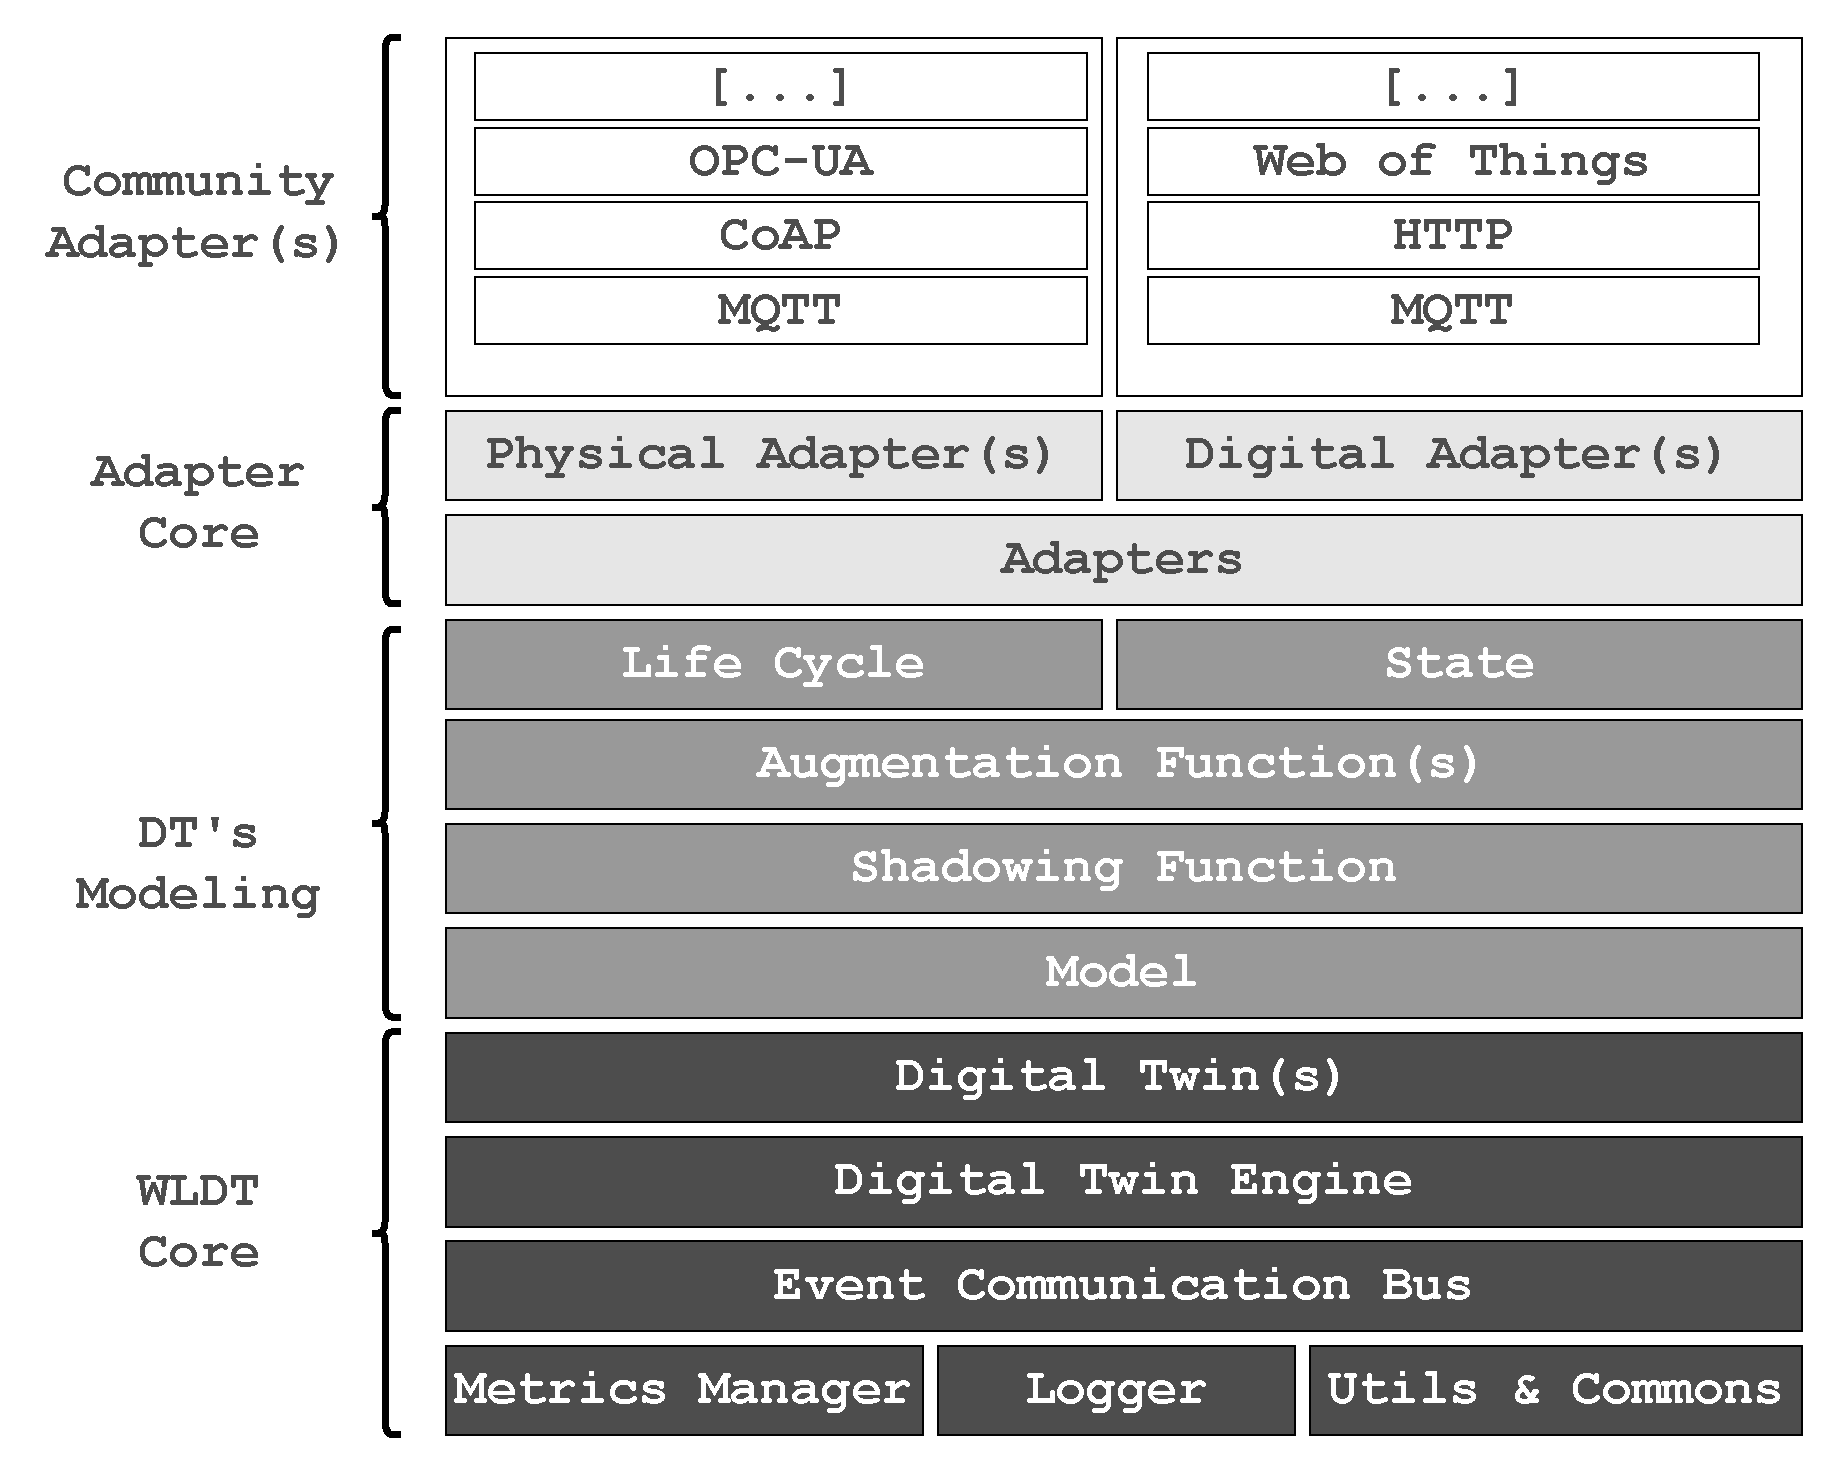
\includegraphics[width=0.7\textwidth]{figures/wldt_architecture.pdf}
    \caption{WLDT Framework's Software Architecture.}
    \label{fig:wldt_architecture}
\end{figure}

The concepts introduced in the previous sections have been implemented in an extended and evolved version of the \acf{WLDT} framework (originally introduced in \cite{PICONE2021100661}) offering a modular DT software architecture designed to maximize flexibility, promote portability, and enable seamless integration across diverse physical assets in diverse application domains.
%
\ac{WLDT} is an open-source Java framework available on GitHub\footnote{\url{https://wldt.github.io}}.

The \ac{WLDT} framework has been re-designed and extended with key requirements:
\begin{itemize}
    \item \textbf{Simplicity}: to facilitate the creation of \ac{DT} instances using existing modules or custom behaviors for specific scenarios;
    \item \textbf{Extensibility}: to allow easy extension of the \ac{DT} \ac{API}, enabling customization and addition of new features through concurrent module execution;
    \item \textbf{Portability \& Microservice Readiness}: to ensure that \ac{DT}s can run on any platform without modifications, supporting deployment as independent microservices.
\end{itemize}

The main components of the \ac{WLDT} architecture are illustrated in \Cref{fig:wldt_architecture}, which outlines the three architectural levels: the core library, the DT model, and the implementation of physical and digital interfaces through \ac{PhA} and \ac{DiA} (\Cref{sec:dte:engineering-dt:physical-digital-adapters}).

The \textit{Metrics Manager} provides the functionalities for managing and tracking various metrics within DT instances, combining both internal and custom metrics through a flexible and extensible approach.
The \textit{Logger} is designed to facilitate efficient and customizable logging within implemented and deployed DTs, with configurable log levels and versatile output options.
The \textit{Utils \& Commons} component contains a collection of utility classes and common functionalities that can be readily employed across DT implementations, ranging from handling common data structures to providing helpful tools for string manipulation.

The \textit{Event Communication Bus} represents the internal Event Bus, designed to support communication between the different components of the \ac{DT} instance (\ac{PI}, \ac{M} and \ac{DI}).
%
It allows for the definition of customized events to model both physical and digital inputs and outputs. Each \ac{WLDT} component can publish on the shared Event Bus and define a filter to specify which types of events it is interested in managing, associating a specific callback to process different messages.

The \textit{Digital Twin Engine} defines the multi-threaded engine of the library, allowing the execution and monitoring of multiple \acp{DT} and their core components simultaneously.
It orchestrates the different internal modules of the architecture while keeping track of each one, and it serves as the core of the platform, enabling the execution and control of deployed \acp{DT}.
Currently, it supports the execution of multiple twins within the same Java process, but the same engine abstraction could extend the framework to support distributed execution through different processes or microservices.

The DT component consists of a modular structure within \ac{WLDT}, combining core functionalities and capabilities of physical and digital adapters.
%
Each DT's core module is its \textit{Model}, which is responsible for implementing the twin's behavior over time. This model controls both the \textit{Shadowing Function} and \textit{Augmentation Function(s)}.
%
The Shadowing Function manages the digitalization process by integrating data from physical adapters and action requests from digital adapters.
It maintains the DT's \textit{State}, organizing properties, events, actions, and relationships as introduced in \Cref{sec:dte:engineering-dt:abstract-architecture}.
%
Augmentation Functions enhance physical capabilities by introducing new properties and actions through intelligent functionalities or dedicated processing (e.g., anomaly detection or data aggregation).
The DT's core is managed by the library to ensure consistency and lifecycle management, adapting to computational phases and interactions with physical and digital realms via adapters. 

\ac{WLDT} implements functionalities to manage the \ac{DT} synchronization lifecycle as described in \Cref{sec:dte:engineering-dt:dt-lifecycle}, ensuring proper transitions between phases and maintaining alignment with the physical asset's lifecycle.
%
Within the \ac{DT} core, the \emph{Shadowing Function} is responsible for receiving \acp{PAD} from \acp{PhA} and processing them to define when the \ac{DT} can be considered correctly \texttt{Bound} and when the \ac{DT} can be considered \texttt{Synchronized}, starting the \ac{DT} state computation. 

Developers can either leverage existing adapters---customized through configuration for context-specific reuse---or create new ones tailored to their specific requirements.
Each adapter has an internal dedicated lifecycle within the DT to ensure it can start, setup the necessary resources and respond to incoming events appropriately.
%
Adapters are identified by unique IDs, enabling the library to coordinate multiple adapters, adjust logs, and execute functions upon receiving new events. 
%
\ac{DiA} have direct access to the \ac{DT}'s state as well as the \ac{DT} history through callbacks or synchronous access, allowing it to retrieve information and expose it to digital consumers through various protocols according to the application context.


%========================================================
\section{Evaluation of the Proposed Approach}
%========================================================

In this section, the proposed architectural approach for engineering \acp{DT} is evaluated through the implementation of an industrial scenario.
%
This showcase demonstrates the practical application of the concepts introduced in the previous sections and highlights the benefits and challenges of the approach in a real-world context.

%-------------------------------------------
\subsection{Industrial Scenario Description}
%-------------------------------------------

As a reference scenario, a manufacturing setting where \ac{DT} are deployed to monitor and manage a production line is considered. 
%
The production line is realized through the \emph{Fischertechnik Training Factory Industry 4.0}\footnote{Fischertechnik Industry \& Universities: \url{https://www.fischertechnik.de/en/products/industry-and-universities}}, controlled by PLCs that publish real-time data via OPC-UA and integrated with Arduino RP2040 boards\footnote{Arduino RP2040: \url{https://docs.arduino.cc/hardware/nano-rp2040-connect/}} for accelerometer data collection and processing and communicating over MQTT.
This microfactory setup provides a controlled yet dynamic environment for testing and refining DT technologies in a realistic industrial context.

\begin{figure}[t]
    \centering
    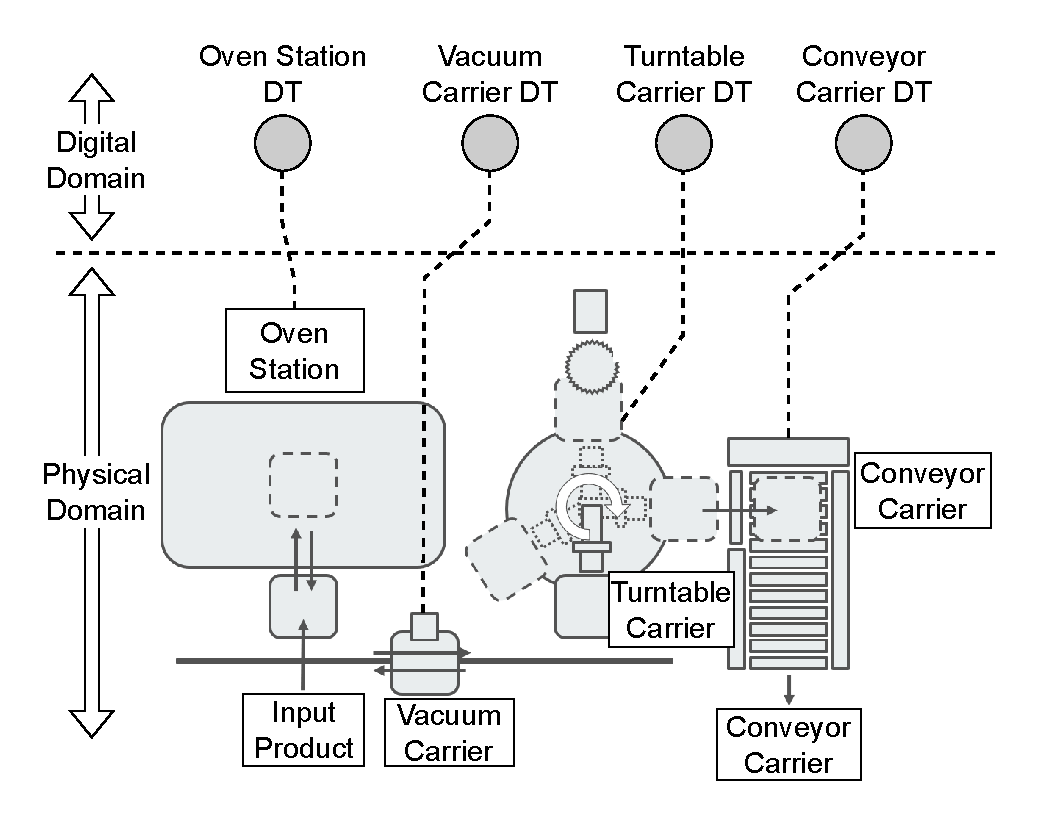
\includegraphics[width=0.75\columnwidth]{figures/engineering-wldt/fischer-layout-first-level-dt.pdf}
    \caption{A schematic view of the Multiprocess Station with Oven of the target industrial scenario.}
    \label{fig:fischer-dt-first-level}
\end{figure}

In this scenario, pieces are processed along a production line, passing through multiple machines.
%
The first station, referred to as the \textit{Multiprocess Station with Oven}.
As shown in \Cref{fig:fischer-dt-first-level}, the module consists of five machines arranged in a flow shop layout: 
three material handling units (vacuum gripper carrier, turntable, and conveyor)
and two transformation stations (oven and saw station).
%
Each machine is equipped with sensors (light barriers and limit switches) and actuators (with two or three operational states).
%
The second station, named the \textit{Indexed Line}, comprises four conveyor belts, two of which include mechanical processing operations for the workpieces.

The goal of the scenario is to implement, through \acp{DT}, a system with the following desired features: 
\begin{itemize}
    \item monitor the state of each machine in the production line;
    \item track production performance, including the number of pieces processed and the efficiency of each machine;
    \item monitor power consumption of each machine to optimize energy usage;
    \item regulate the production speed of each machine to ensure smooth operation and avoid bottlenecks;
    \item compute the overall production performance of the entire production line;
    \item compute the overall energy consumption of the entire production line;
    \item manage external action requests, at the system level, to adjust production parameters or respond to specific events;
\end{itemize} 

%--------------------------------------------
\subsection{Digital Twin System Architecture}
%--------------------------------------------

To achieve the desired features, a multi-layered architecture is proposed, consisting of machine-level, department-level, and factory-level \acp{DT}.
%
Each machine-level \ac{DT} processes incoming data on properties and events to generate insights such as production and energy KPIs, while also managing action requests to regulate their individual speed.
%
Additionally, two department-level \acp{DT} are created, matching the two different goals of tracking energy consumption and production performance.
%
All \acp{DT} are built using the \ac{WLDT} framework.

The production efficiency is computed at the machine level using the \ac{OEE} metric\footnote{OEE: \url{https://www.oee.com/}} calculated from production rate, uptime, and downtime.
%
At the department level, \acp{DT} representing the Indexed Departments assess performance by computing Weighted \ac{OEE}~\cite{OEE-manufacturing-cell-Gamberini-2017,Introduction-to-TPM-total-productive-maintenance-Nakajima-1995}, derived from individual machine \acp{DT}, and track throughput, defined as processed pieces per unit time.
Throughput is determined by monitoring entry and exit events within the department, utilizing relationships captured by the associated \acp{DT}.

\begin{figure}
    \centering
    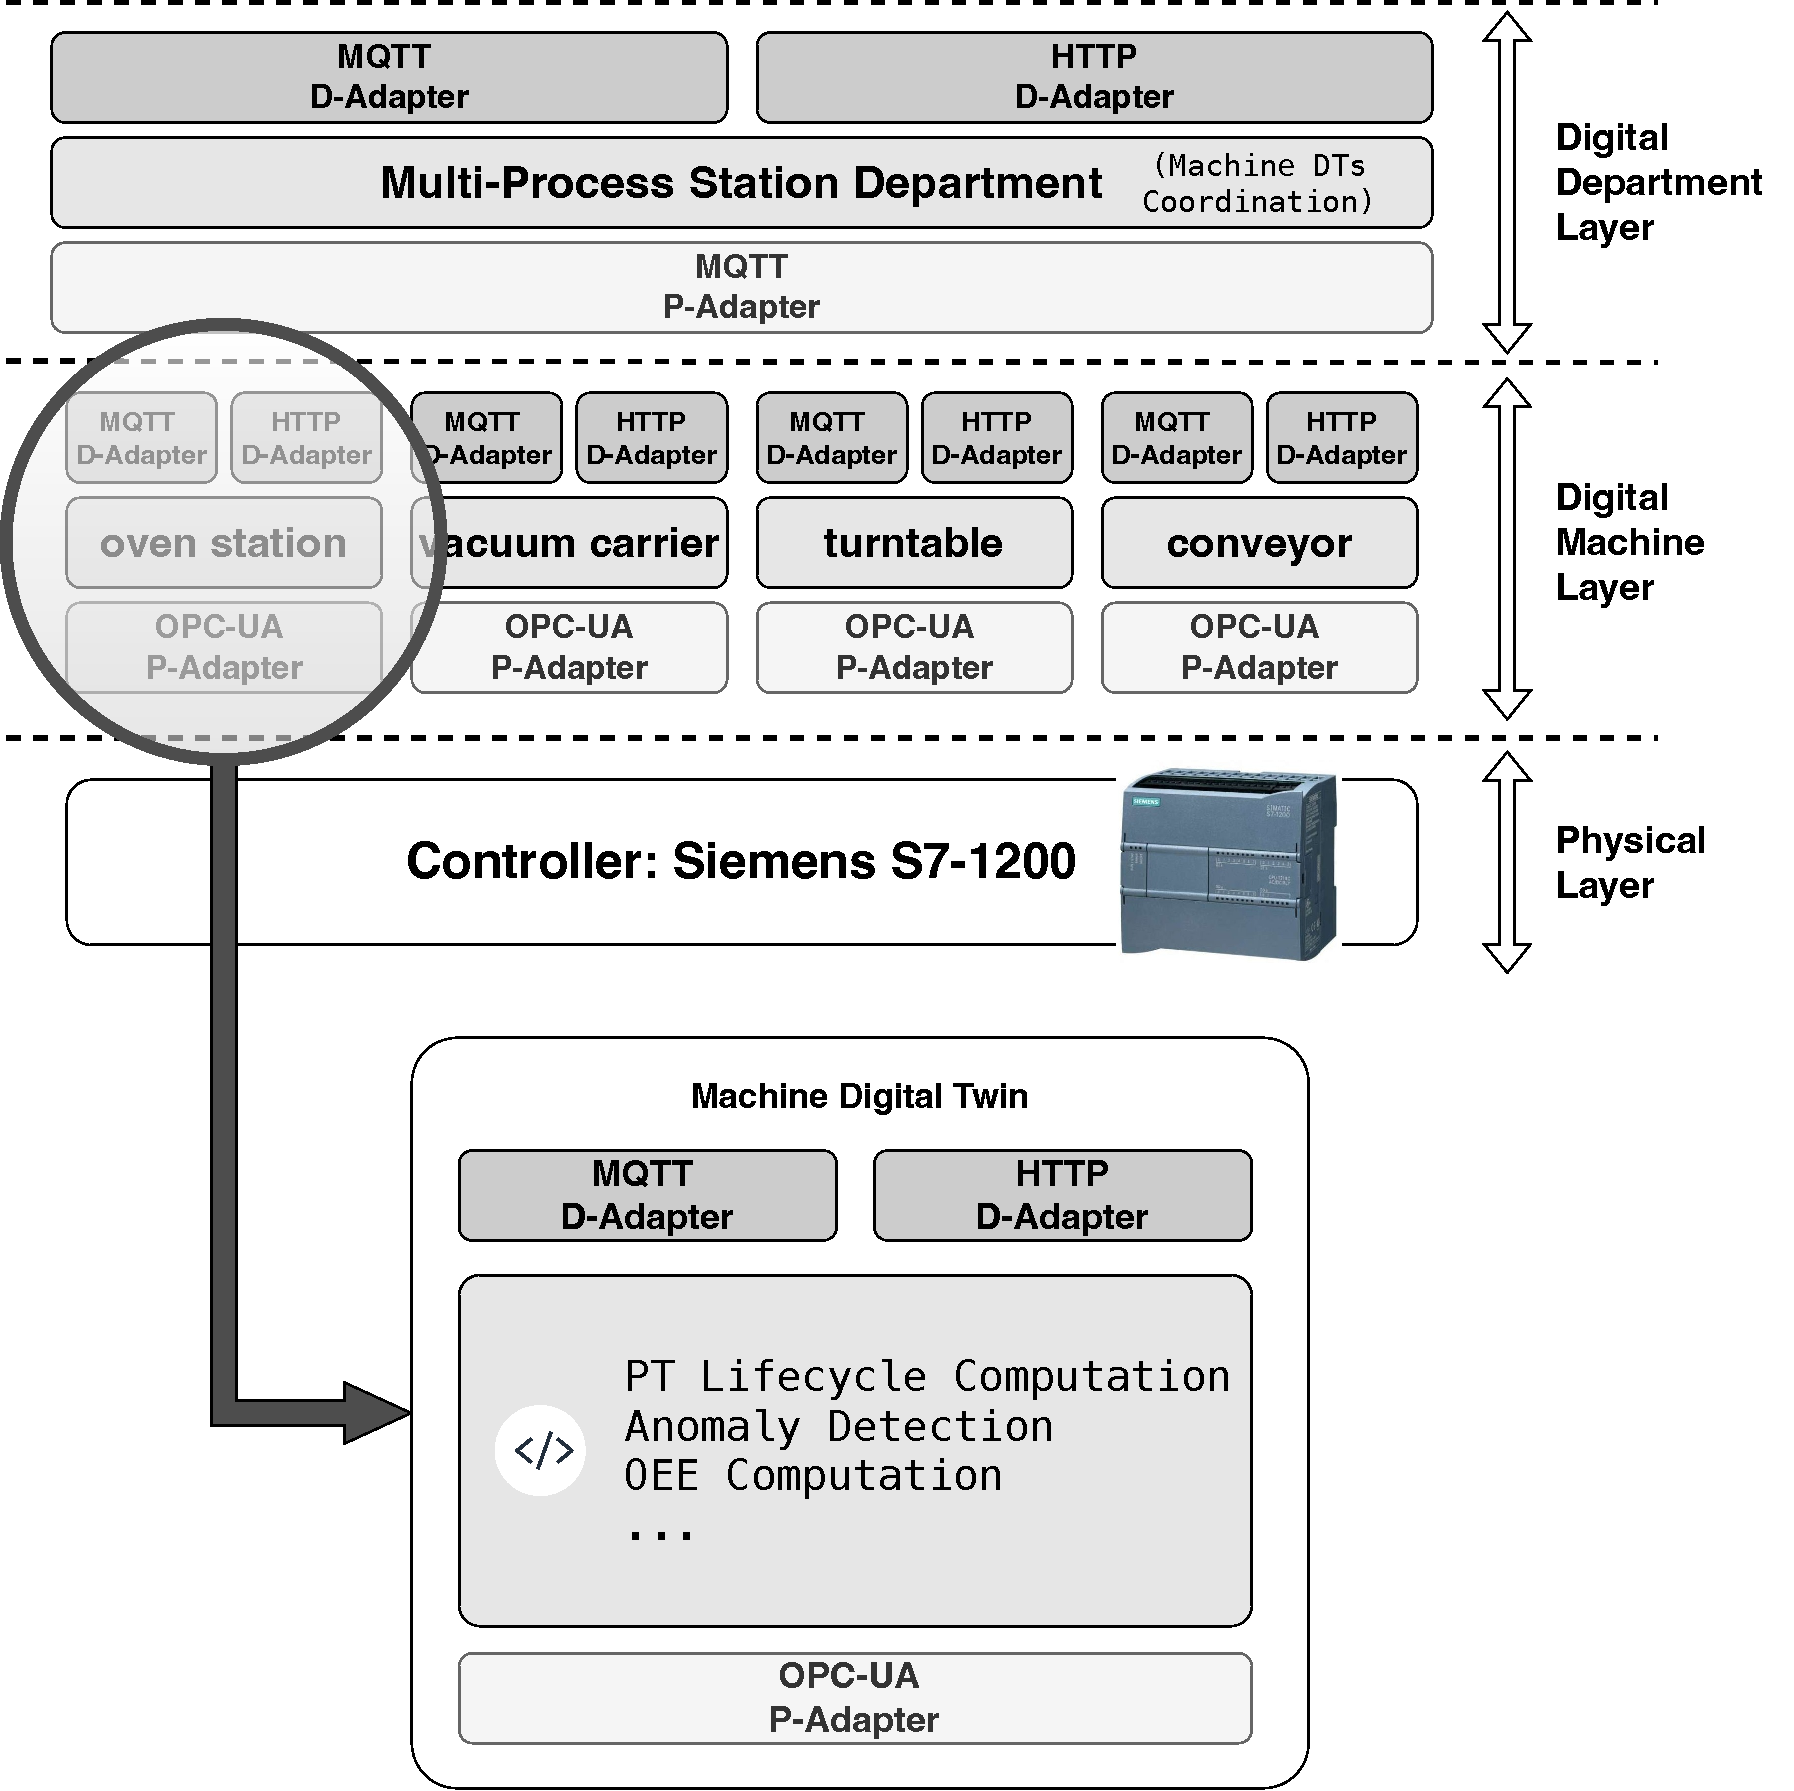
\includegraphics[width=0.7\textwidth]{figures/dt-lifecycle/mps_dt_structure_2.pdf}
    \caption{Multiprocess Station Digital Twin architecture overview.}
    \label{fig:multiprocess-station-dt-structure}
\end{figure}

\Cref{fig:multiprocess-station-dt-structure} shows the resulting \ac{DT} system architecture for the \textit{Multiprocess Station with Oven}.
%
Each machine of the station is represented by a dedicated \ac{DT} which connects to the physical asset through a \ac{PhA} that interacts with the PLC iva OPC-UA.
%
At the department level, the \ac{DT} of the \textit{Multiprocess Station with Oven} aggregates data from the machine-level \acp{DT}, computing overall performance metrics and exposing department-level actions.

\begin{figure}
    \centering
    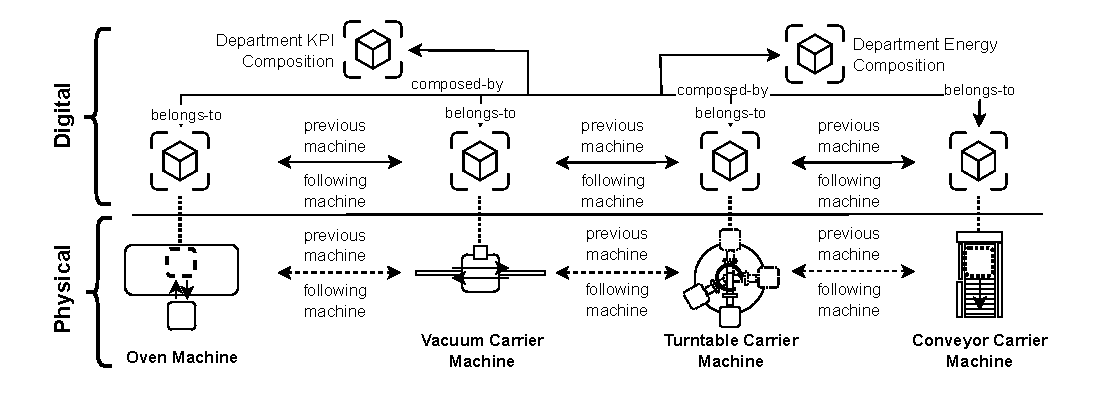
\includegraphics[width=\textwidth]{figures/engineering-wldt/Fischer-relationships.pdf}
    \caption{Relationships between \acp{DT} in the Multiprocess Station serve the purpose of tracking the physical relationships between different machines at the digital level.}
    \label{fig:dt-assets-relationships-overview}
\end{figure}

Figure \Cref{fig:dt-assets-relationships-overview} illustrates the relationships among the various \acp{DT} in the Multiprocess Station.
%
Relationships between machines and DTs (e.g., \emph{previous}, \emph{following-machines}, \emph{is-part-of}) are statically defined in this setting, but are used by department-level \acp{DT} do track the flow of pieces and compute throughput and total pieces processed.
%
\begin{figure}
    \centering
    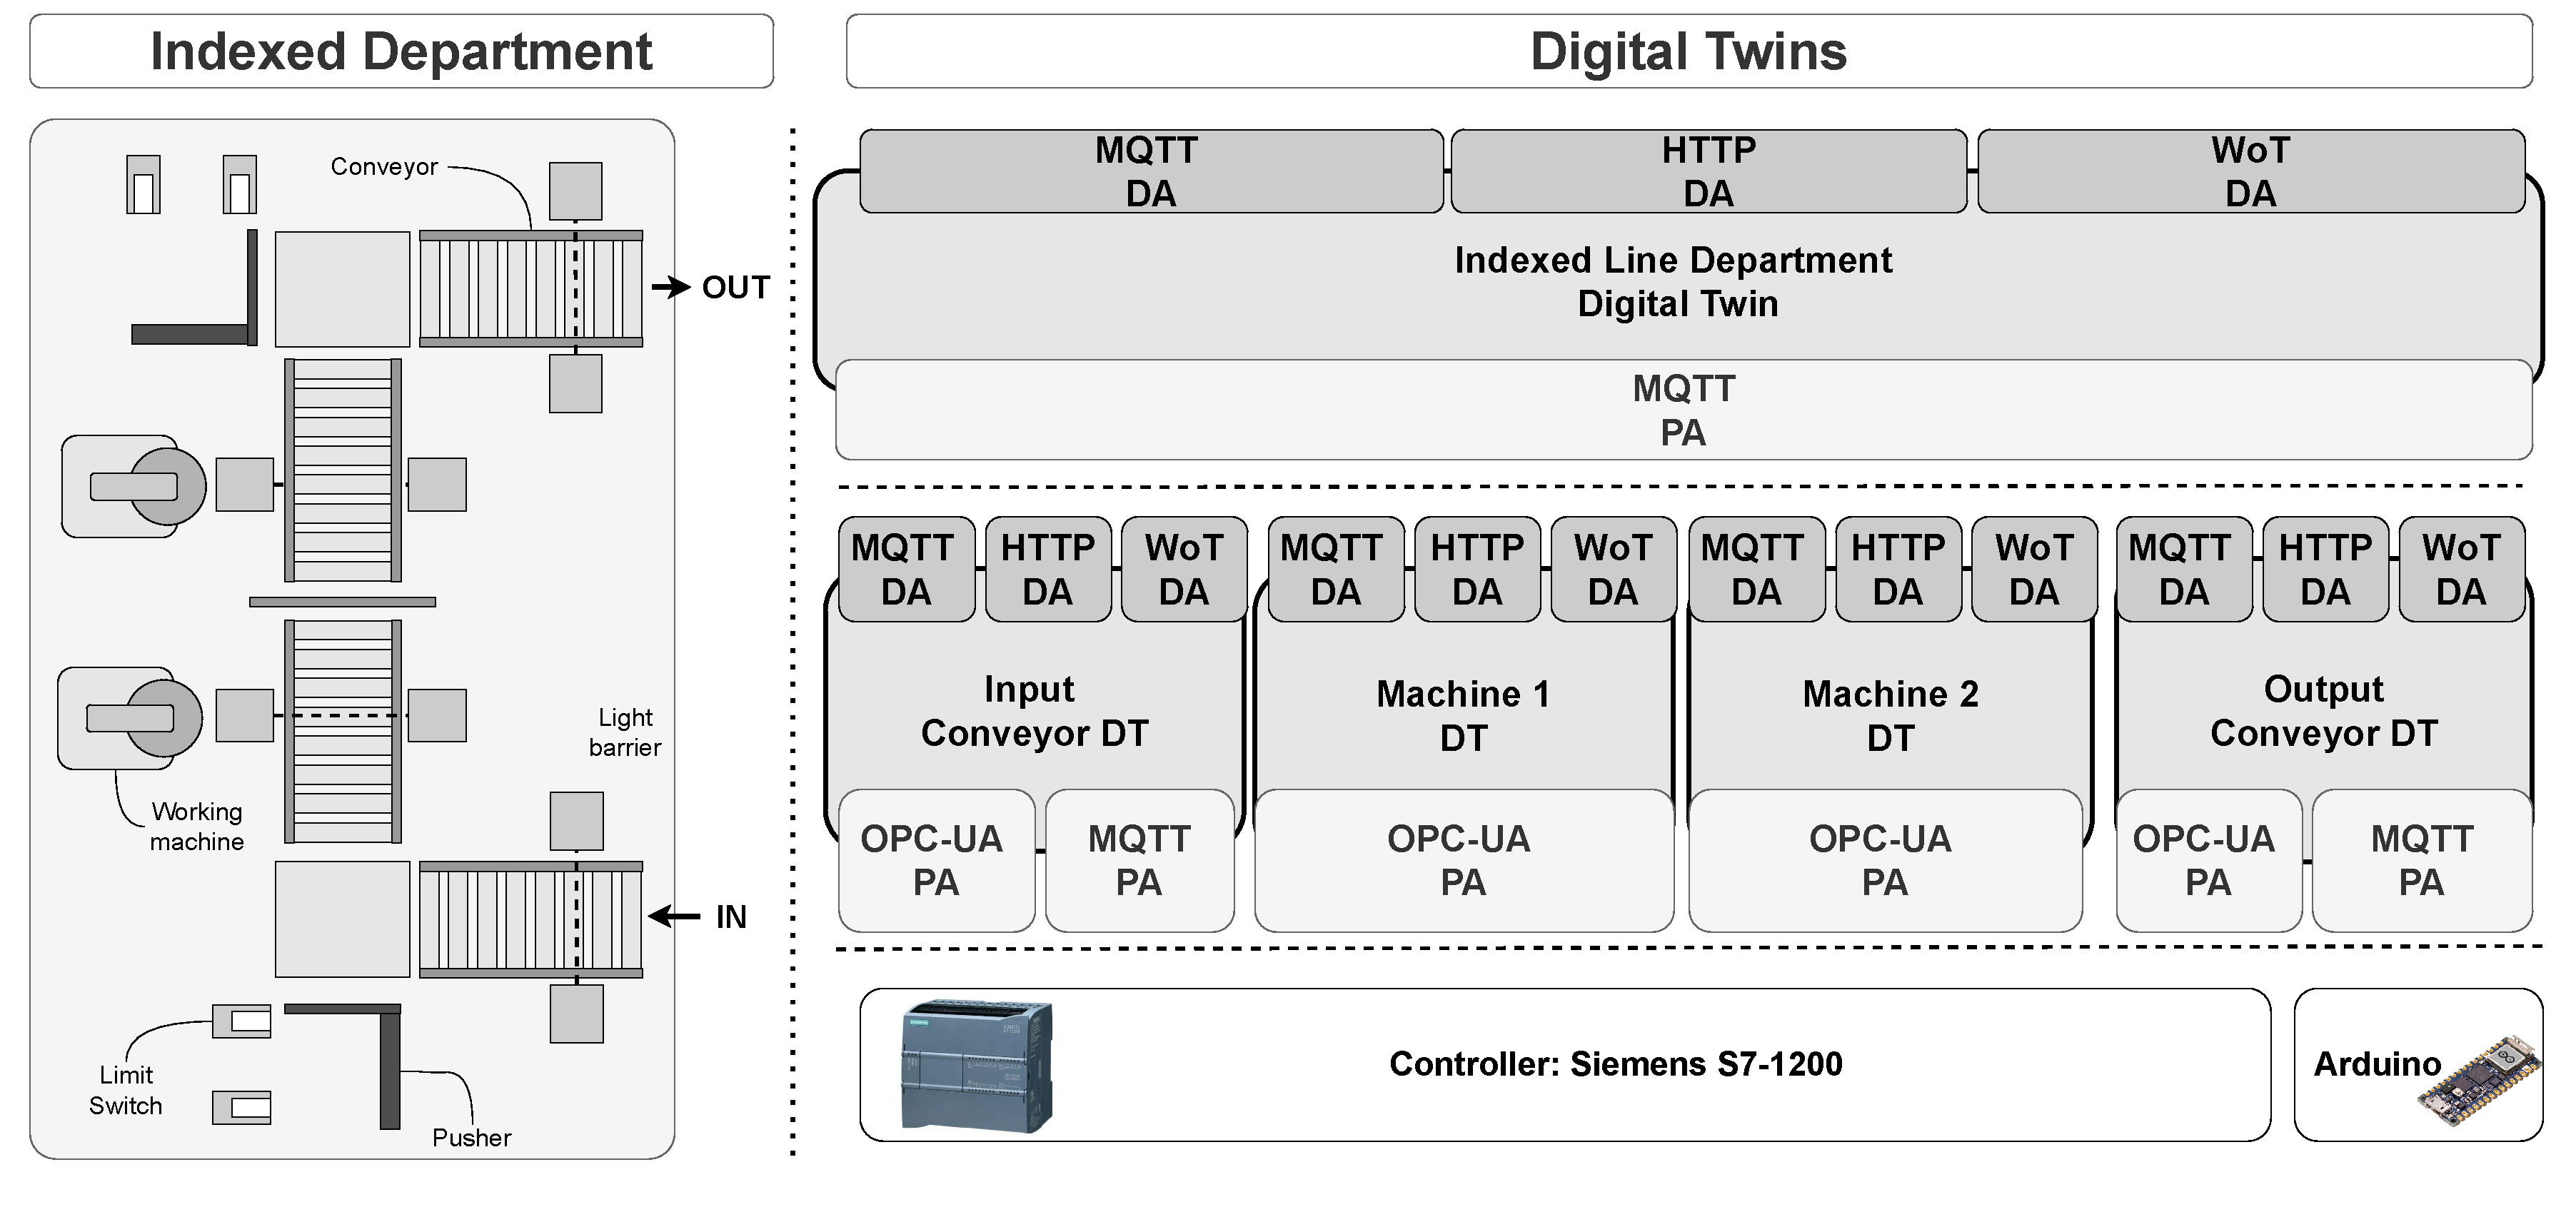
\includegraphics[width=\textwidth]{figures/dt-interoperability/mf_dt_structure.pdf}
    \caption{The \acl{DT} ecosystem architecture of the Indexed Department, alongside a schematic representation of the conveyors.}
    \label{fig:indexed-department-dt-structure}
\end{figure}

Similarly, \Cref{fig:indexed-department-dt-structure} illustrates the \ac{DT} ecosystem architecture for the \textit{Indexed Line Department}. Again, each machine is represented by a dedicated \ac{DT} connected to the physical asset through \acp{PhA}. In this setup, machines integrate the communication of the PLC via OPC-UA and Arduino boards via MQTT.
%
Finally, a factory-level \ac{DT} aggregates data from both departments, 
computing the overall production performance and energy consumption.


Machine Level \acp{DT} expose a digital interface through \acp{DiA}. 
%
An MQTT digital interface is used to connect machine-level \acp{DT} to the department-level \ac{DT}, enabling composition between \acp{DT} in a hierarchical structure. 
%
All \acp{DT} also expose an \ac{HTTP} digital interface which serves as the primary access point for external applications and services.
%
The \ac{HTTP} interface can further be described using \ac{WoT} \acp{TD}, enabling seamless integration with other \ac{WoT}-compliant systems and applications as discussed in \Cref{sec:dte:dt-engineering:wot-for-dt}.

%-------------------------------------------------------------------------
\subsection{Reducing Complexity through Reusable Adapters}
%-------------------------------------------------------------------------

Notably, the physical and digital adapters that implement MQTT, OPC-UA, and HTTP protocols, along with \ac{WoT} over HTTP for serving \acp{TD}, are reusable across different instances.
These adapters, through configurable parameters, enable effective communication and integration within both digital and physical environments.

Upon startup, each \ac{DT} connects to its data source, publishes the \ac{PAD} of the physical asset, and interacts with the PLC or Arduino to collect and send data, enabling digitalization and interoperability among heterogeneous equipment. 

%%%
\begin{figure}
    \centering
    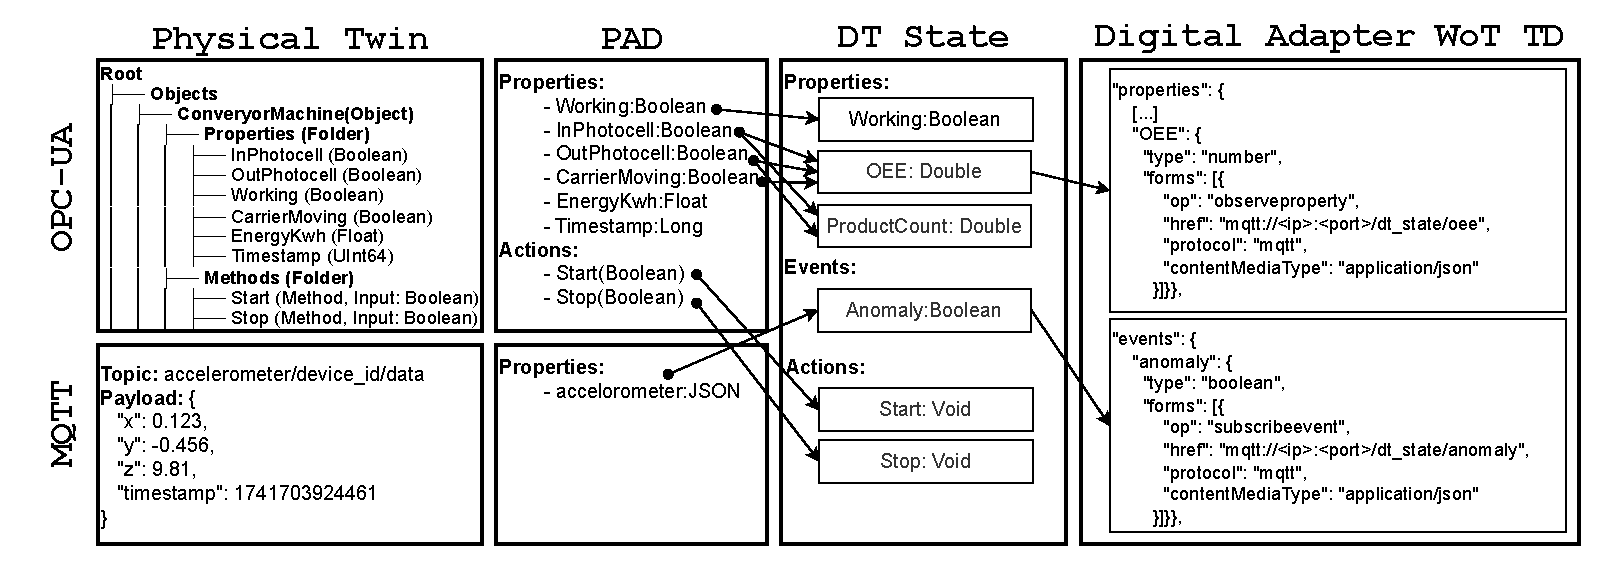
\includegraphics[width=\textwidth]{figures/dt-interoperability/dt_interoperability-pad_dt_wot.pdf}
    \caption{The transition from physical to digital representation via the \ac{PAD}, the \ac{DT} State, and the \ac{DTD} for external consumers.}
    \label{fig:pad_dt_wot}
\end{figure}
%%%


\Cref{fig:pad_dt_wot} schematically illustrates the evolution of data and representation from the physical to the digital realms through the adoption of the proposed \ac{DT} architectural approach, \ac{PAD} integration, and \ac{WoT} \acp{TD} used as \acp{DTD} on the digital side, specifically for the output conveyor of the Indexed Department production line (\Cref{fig:indexed-department-dt-structure}).
On the physical side, data is structured using OPC-UA with a hierarchical organization, containing telemetry data and action methods mapped to specific data types.
Accelerometer data is transmitted over MQTT on a specific topic with a JSON payload containing axis acceleration values. 

The \acp{PAD} act as an intermediary, translating data from the PT into a format suitable for the DT core, decoupling it from the complexity of interacting with the \ac{PT} and enabling discovery, understanding, and utilization of available data and methods.
Using the information from the \acp{PAD}, the \ac{DT} model computes the \ac{DT}'s state with target properties, events, and actions, based on either one-to-one matching of physical characteristics or augmented by combining multiple physical properties into computed \ac{DT} properties or events, such as computing the value of the \ac{OEE} property or triggering anomaly detection events based on accelerometer data. 

Finally, the \ac{DiA} of the \ac{DT} leverages \ac{WoT} \ac{TD} to describe the DT's data and functionalities through a standardized, interoperable, and machine-readable approach.
The \ac{TD} specifies how these can be accessed via protocols and data formats.
This approach enables effective interoperability from the physical to the digital, using a modular and decoupled structure through \acp{DT} in the target industrial use case.

This deployment aims to measure the impact of digitization and responsibility decoupling by comparing the system complexity in scenarios with and without \ac{DT} adoption and also with respect to the different \ac{DT}'s architectural layers.
%
This allows to assess the benefits of a modular, structured DT-based approach, particularly in terms of interoperability and heterogeneity management.

To quantify how effectively the proposed approach of \ac{PhA} and \ac{DiA} manages cyber-physical heterogeneity,
the \textit{Cyber-Physical Complexity Index (CP-CI)} proposed in \cite{lippi_dt_causality_learning, LOMBARDO2024107203} is adopted as a measure of complexity of the system. 

The CP-CI quantifies the perceived complexity of a cyber-physical application based on:
\begin{itemize}
    \item \textit{Required Protocols (p)}: communication protocols needed for device interaction;
    \item \textit{Communication Patterns (c)}: interaction models (e.g., Publish/Subscribe, Request/Response);
    \item \textit{Data Formats (d)}: required data representations or serialization methods;
    \item \textit{Interaction Points (n)}: modules or services involved in data exchange; and
    \item \textit{Aggregation Points (a)}: levels of abstraction for physical data (e.g., merging data from multiple machines).
\end{itemize}
Each criterion is weighted with a \textit{Criteria Importance Factor} (\(CIF\)) from 1 (low) to 3 (high), indicating its impact on development, deployment, and maintenance.

Focusing on \ac{DT} interoperability, the CP-CI is extended to include both inbound and outbound interfaces, essential for bridging the physical and cyber layers with differing requirements.
This extension enables a more precise assessment of the complexity in managing interoperability across system boundaries.
The CP-CI was applied not only to the entire \ac{DT} but also to its internal layers: \ac{PI}, Core, and \ac{DI}.
These results were compared to those of a monolithic external application that directly handles business logic and interoperability, bearing the full complexity, highlighting the advantages of the modular \ac{DT} design.
High importance ($CIF=3$) was assigned to managing heterogeneous data formats ($d$) and aggregation points ($a$), as they are crucial for creating interoperable data models.
Medium importance ($CIF=2$) was given to protocol diversity ($p$) and interaction with multiple entities ($n$), which become more significant as systems scale.
Low importance ($CIF=1$) was assigned to multiple communication patterns ($c$), as their concurrent use is standard in distributed applications.


\begin{figure}
  \centering
  \begin{subfigure}[t]{0.32\linewidth}
      \centering
      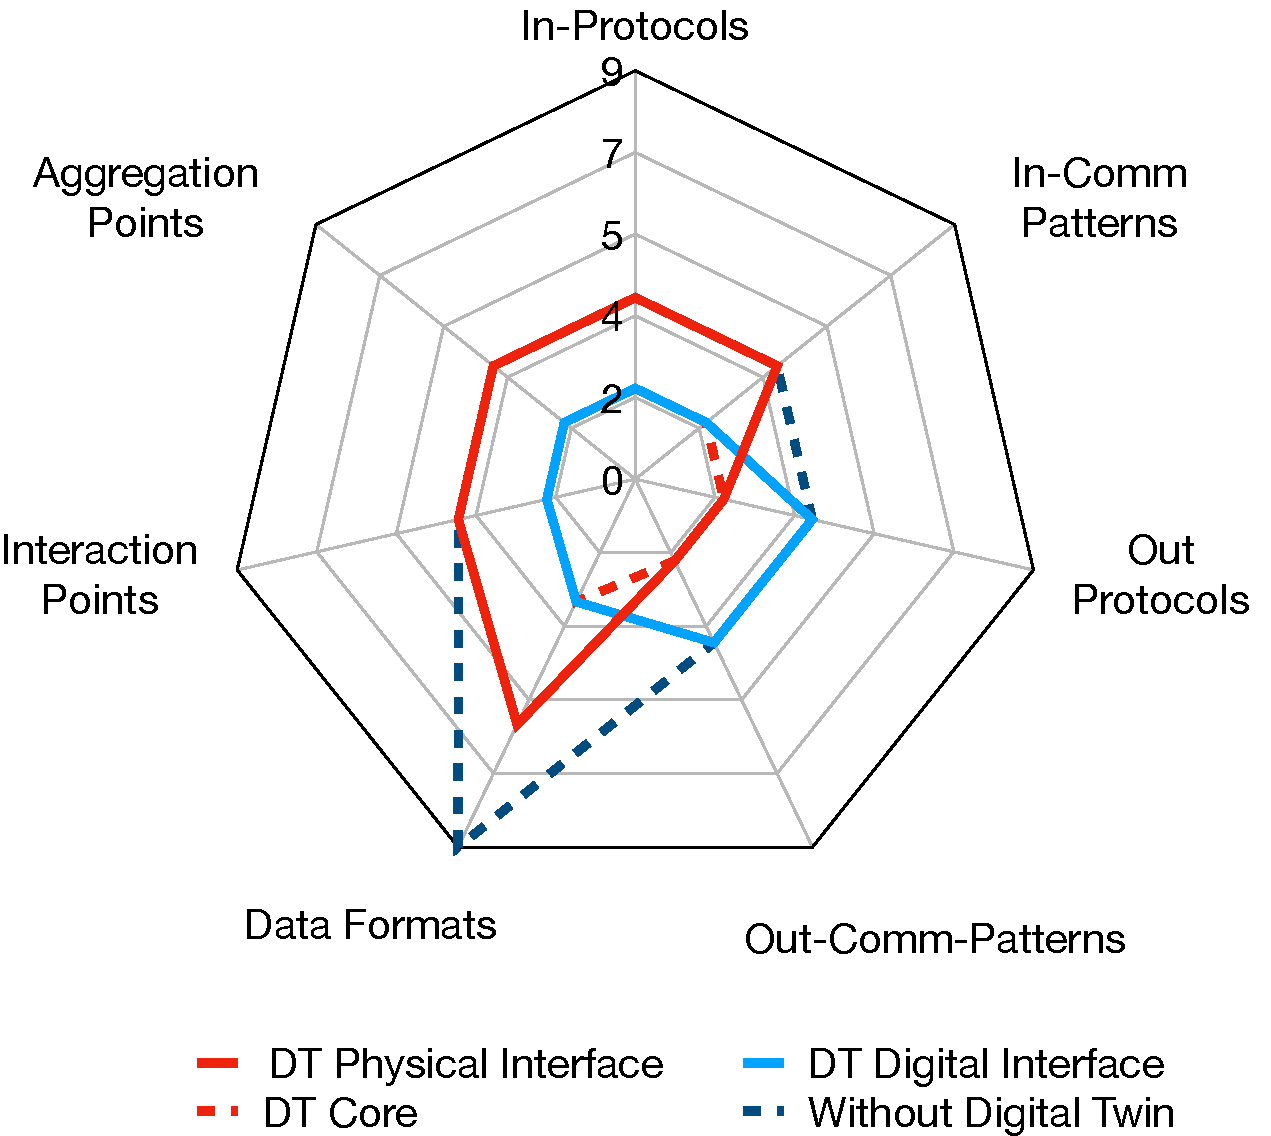
\includegraphics[width=\linewidth]{figures/dt-interoperability/machine_complexity_index.pdf}
      \caption{Machine Digital Twin}
      \label{fig:machine_complexity_index}
  \end{subfigure}
  \begin{subfigure}[t]{0.32\linewidth}
      \centering
      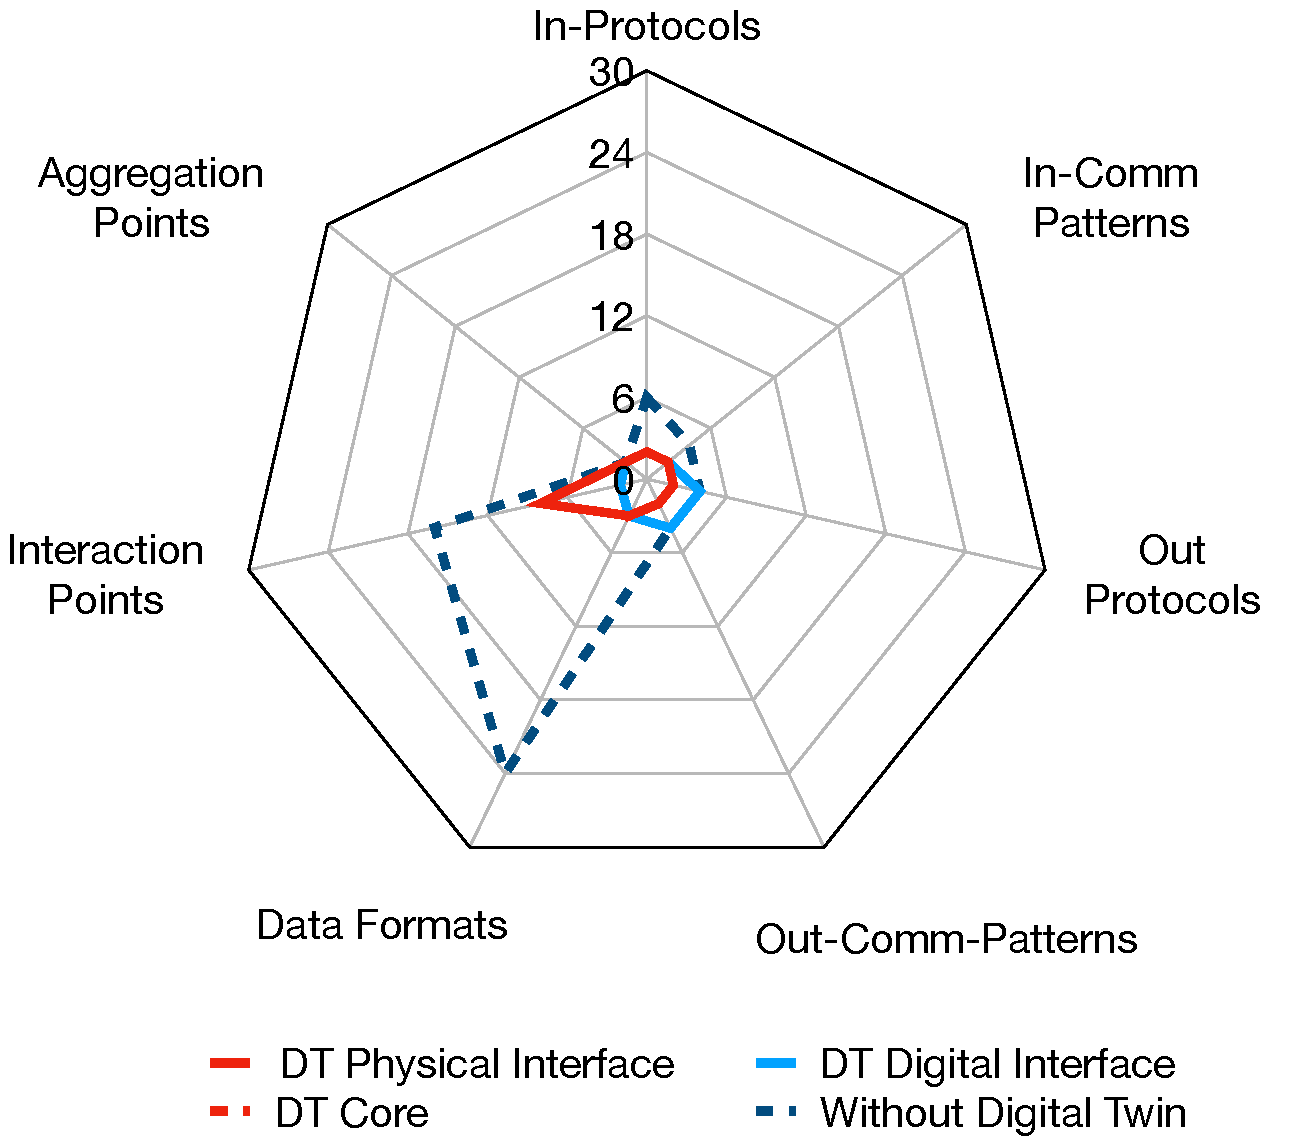
\includegraphics[width=\linewidth]{figures/dt-interoperability/station_complexity_index.pdf}
      \caption{Station (Indexed-Line) Digital Twin}
      \label{fig:station_complexity_index}
  \end{subfigure}
  \begin{subfigure}[t]{0.32\linewidth}
      \centering
      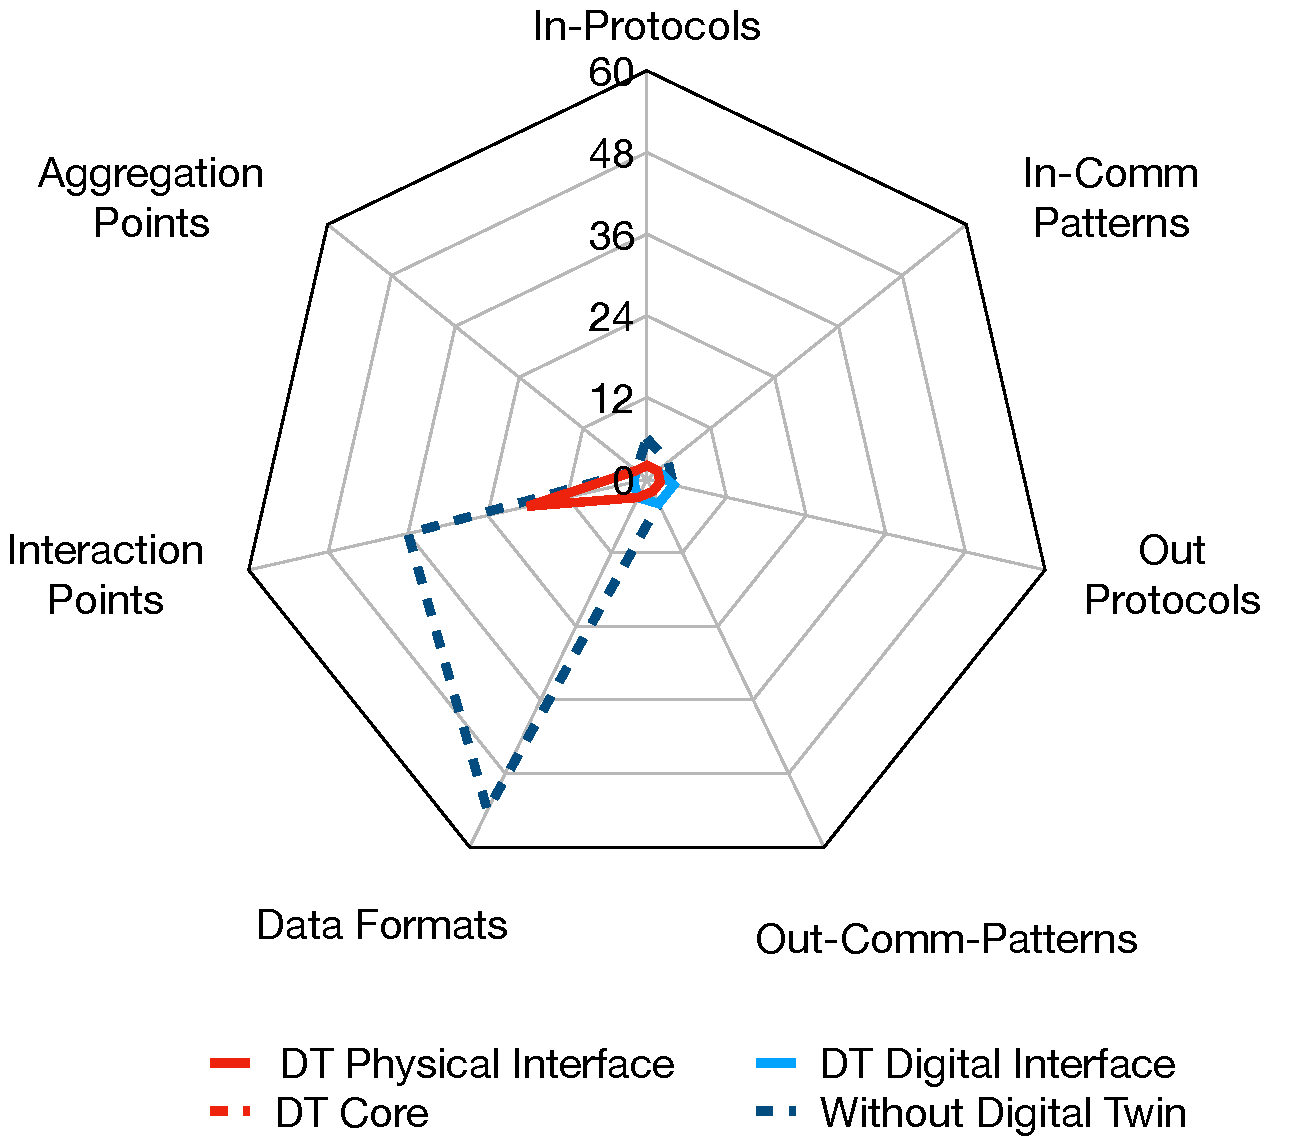
\includegraphics[width=\linewidth]{figures/dt-interoperability/factory_complexity_index.pdf}
      \caption{Factory Digital Twin}
      \label{fig:factory_complexity_index}
  \end{subfigure}
  \caption{Schematic representation of cyber-physical complexity and its impact on various components.}
  \label{fig:dt_complexity_index}
\end{figure}


The graphs presented in \Cref{fig:dt_complexity_index} display the CP-CI values obtained across different levels of deployment: a single machine, the indexed department, and the entire factory.
%
For the machines analyzed, the involved protocols ($p$) and communication patterns ($c$) are both set to 2, as MQTT and OPC-UA are used with Pub/Sub and Request/Response interactions.
On the digital side, both MQTT and HTTP are employed.
Regarding data formats ($d$), each machine manages 2 distinct formats, accounting for both PLC data and Arduino accelerometer information.
Furthermore, the interaction points ($n$) and aggregation points ($a$) are both 2, reflecting the aggregation and interaction with two different sub-entities for each machine and its corresponding DT.

The results for single machines (\Cref{fig:machine_complexity_index}) highlight the critical role of the \ac{PI} in the \ac{DT} architecture.
As a decoupling layer, the \ac{PI} isolates physical-world complexities from the DT core, managing priorities like protocols, data formats, interaction points, aggregation strategies, and communication patterns.
This allows the DT core to focus on uniform data, processed through the interface via \ac{PAD} and payload transformations, without dealing with heterogeneous physical entities.
%
Consequently, the core interacts only with its internal communication pattern and consistent interaction points, regardless of the physical environment's configuration.
A similar approach is applied to the \ac{DI}, which is decoupled from physical complexities and adapts to external digital systems, ensuring modularity and reuse.

In contrast, systems without a \ac{DT} must embed all heterogeneity management into a single application, burdening it with business logic, protocol diversity, and data format interoperability.
This increases complexity and reduces scalability, as reflected by the complexity index parameters.

As system architecture scales from individual machines to departments (Figure \ref{fig:station_complexity_index}), or entire factories (Figure \ref{fig:factory_complexity_index}), protocol diversity stabilizes while the number of interaction points and data formats increases due to the need for managing heterogeneous components.
The complexity measure shows that systems at the department or factory level experience a significant rise in complexity, driven by interaction points, aggregation nodes, and data format diversity.

These results emphasize the benefits of the modular and interoperable approach presented in \cref{sec:dte:engineering-dt:physical-digital-adapters}.
By encapsulating complexity within reusable \emph{adapters} and using interoperable representations, developers can simplify application development.
In contrast, monolithic systems struggle with managing interoperability and system evolution as integration requirements grow.

%---------------------------------------------------
\subsection{Lifecycle Awareness and Coordination}
%---------------------------------------------------

To demonstrate the applicability of the proposed lifecycle synchronization model introduced in \cref{sec:dte:engineering-dt:dt-lifecycle}, 
each machine-level \ac{DT} handles the synchronization between the $LP_{PA}$ and the corresponding $LP_{DT}$.
%
Furthermore, an anomaly detection algorithm runs within each \ac{DT}, enabling it to identify and report issues that the PLC alone might not detect, thus dynamically computing the $LP_{PA}$ when necessary (e.g., when a piece does not reach a reference photocell on the machinery within a predetermined time and an anomaly is consequently detected).

The department-level \ac{DT} of the Multiprocess Station incorporates coordination logic that adjusts machine behavior based on their current phases, ensuring seamless station management.

\begin{figure}
    \centering
    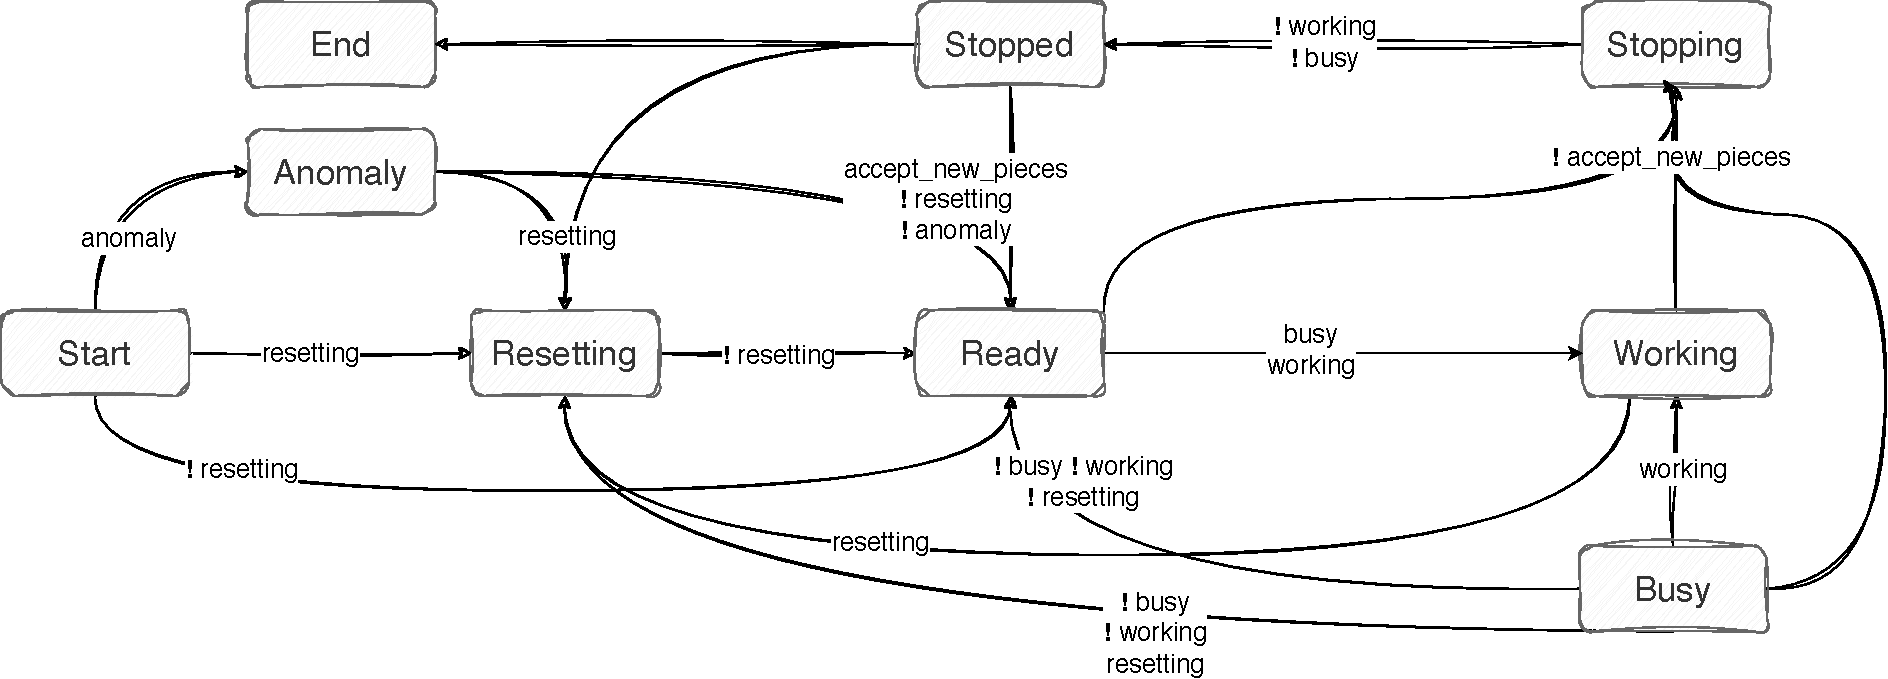
\includegraphics[width=\textwidth]{figures/dt-lifecycle/graph_machine_logic.pdf}
    \caption{Lifecycle of a \ac{PA} in the target industrial scenario, highlighting the different phases that the \ac{DT} needs to account for when synchronized.}
    \label{fig:graph-machine-logic}
\end{figure}

The machine-level \acp{DT} operate based on data produced by their physical counterparts. Leveraging these temporal data, it is possible to model the lifecycle of the physical object within the DT lifecycle as shown in \Cref{fig:graph-machine-logic}.
%
When the DT lifecycle reaches the Synchronized state, it accurately mirrors the corresponding phase of the physical machinery's operation.
%
These phases are inspired by the reference structure for industrial machine phases defined by ISA-95~\cite{ISA95} aligning \acp{DT} with recognized industry standards, enhancing their applicability and effectiveness in real-world industrial settings.

To accurately define the phases of the physical machinery,
it is essential to specify the transition conditions between these phases by leveraging the raw data and telemetry received from sensors and actuators via OPC-UA from the PLC.
%
The DT processes this data to compute and maintain the synchronized lifecycle, ensuring a precise and real-time reflection of the physical object's operational state.

Department-level \acp{DT} enable hierarchical coordination not only between machines within the same station but also across different stations.
%
For example, coordination between the \textit{Multiprocess Station} and the previously mentioned \textit{Indexed Line} can be simplified by establishing consistent lifecycle phases across machines.
%
Without this approach, coordination among multiple DTs requires using low-level physical information and telemetry, making the process less intuitive.

\begin{algorithm}
\caption{Multiple DTs Stopping Procedure}
\begin{algorithmic}
\State \texttt{invoke(OvenDT, STOP)}
\While{ \texttt{OvenDT.phase} \textbf{is not} \texttt{STOPPED} }
    \State \texttt{wait(OvenDT.phase} \textbf{is not} \texttt{WORKING)}
\EndWhile
%\vspace{1em}
%\State \textbf{publish} event ``change-vacuum-gripper-cycle" with value \texttt{false}
\State \texttt{invoke(GripperDT, STOP)}
\While{ \texttt{GripperDT.phase} \textbf{is not} \texttt{STOPPED}}
    %\State \textbf{log} waiting for end of vacuum-gripper \texttt{WORKING} state
    \State \texttt{wait(GripperDT.phase} \textbf{is not} \texttt{WORKING)}
\EndWhile
%\vspace{1em}
%\State \textbf{publish} event ``change-turntable-cycle" with value \texttt{false}
\State \texttt{invoke(TurntableDT, STOP)}
\While{ \texttt{TurntableDT.phase} \textbf{is not} \texttt{STOPPED} }
    %\State \textbf{log} waiting for end of turntable \texttt{WORKING} state
    \State \texttt{wait(TurntableDT.phase} \textbf{is not} \texttt{WORKING)}
\EndWhile
%\vspace{1em}
\State \texttt{invoke(OutputConveyorDT, STOP)}
\end{algorithmic}
\label{code:soft-stop-logic}
\end{algorithm}

As illustrated by \Cref{code:soft-stop-logic}, high-level control logic can be implemented directly leveraging information encapsulated by $LP_{DT}$ mapping the phase and the transitions of the associated physical counterparts $LP_{PA}$. Specifically, the algorithm outlines the steps the department-level DT can take to halt production on the multiprocess station.
By leveraging this additional layer of abstraction, the department-level DT no longer relies on raw sensor data for control operations, enabling a more declarative and effective coordination process, and distributing responsibilities across different DTs.
%
The composite DT leverages the PA lifecycle phases of individual machines to define the overall lifecycle of the entire multiprocess station. This provides a comprehensive overview of each station's operational behavior, enabling more effective and intuitive system management.


%-------------------------------------
\subsection{Performance Evaluation}
%-------------------------------------


\begin{figure}
    \centering
    \begin{subfigure}{0.75\textwidth}
        \centering
        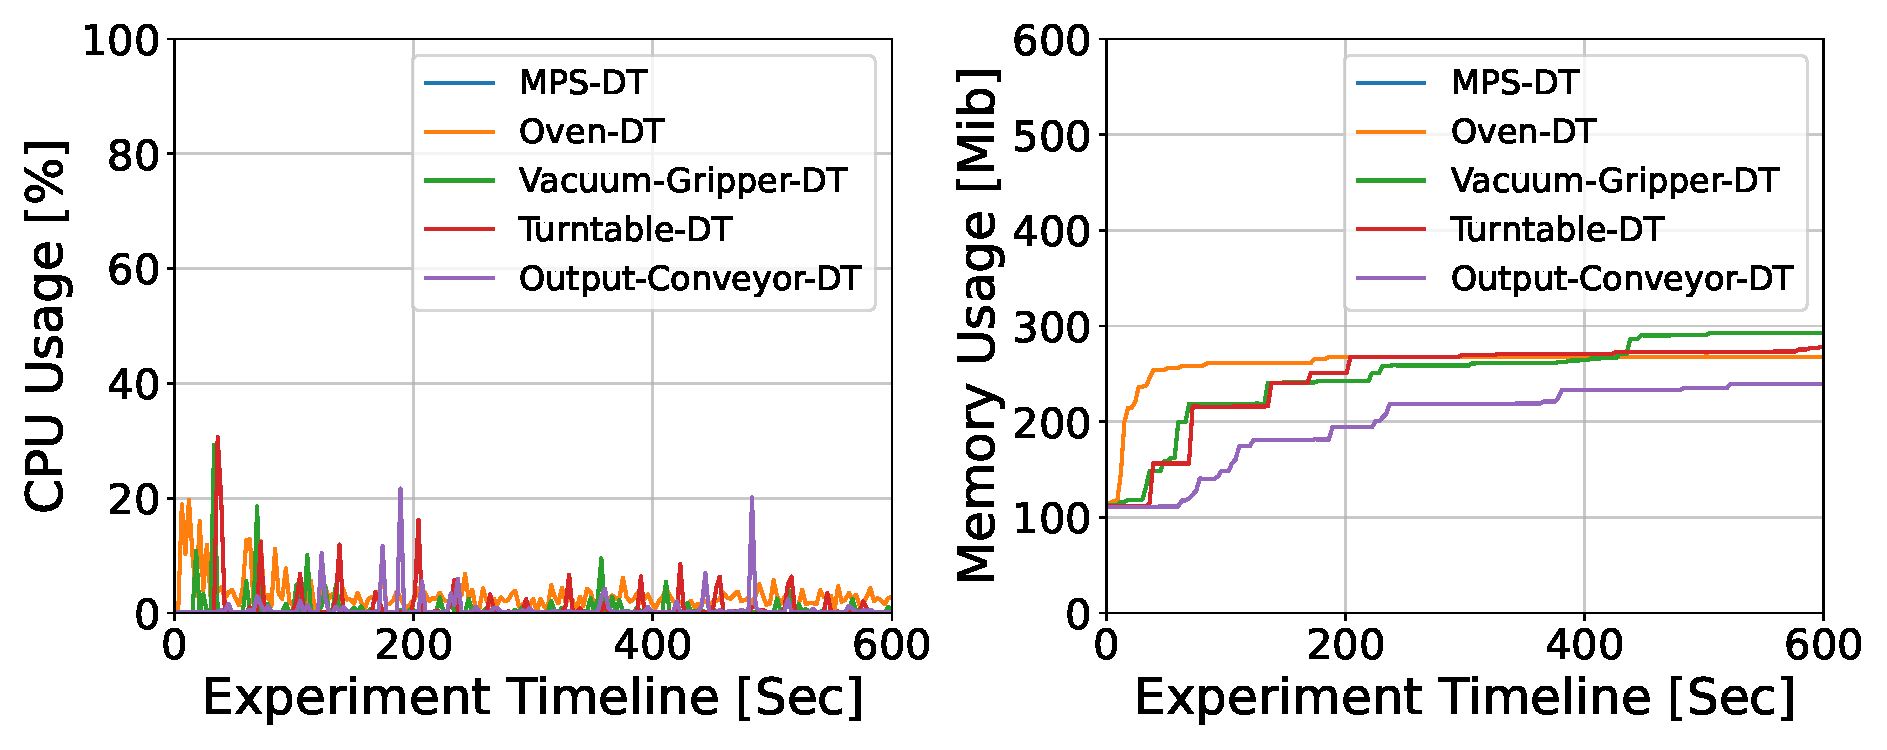
\includegraphics[width=\linewidth]{figures/wldt-results-2.pdf}\\[-2pt]
        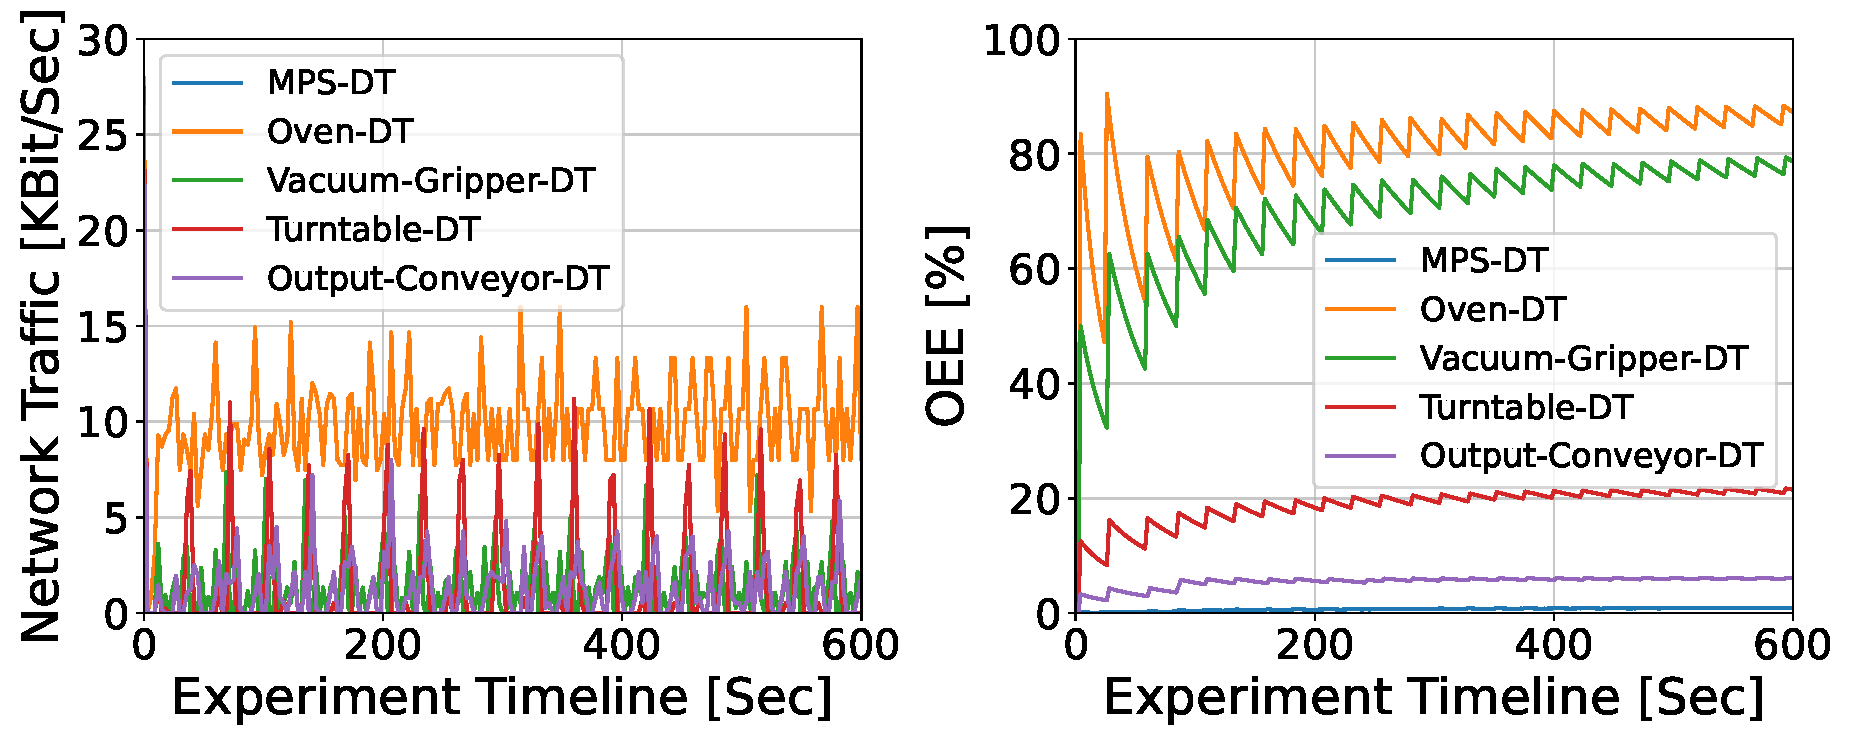
\includegraphics[width=\linewidth]{figures/wldt-results-1.pdf}
    \end{subfigure}
    \caption{Performance indicators of the Multiprocess Station DTs: CPU usage percentage [\%], Memory usage [Mib], Network usage [KBit/sec] and OEE [\%]}
    \label{fig:exp-results}
\end{figure}


To validate the \ac{WLDT} framework,
the \acp{DT} for the Multiprocess Station with Oven were containerized using Docker, and deployed on an Edge node with an Intel i7 2.4GHz processor and 32 GB of RAM.
%
Three key metrics for each DT for a total of 10 minutes (600 seconds):
\begin{itemize}
    \item \textbf{CPU Usage}: the percentage of CPU resources utilized by each DT instance over time;
    \item \textbf{Memory Consumption}: the amount of memory (in MiB) used by each DT instance during its operation;
    \item \textbf{Network Traffic}: the cumulative inbound and outbound network traffic (in Kbit/sec) generated by each DT instance.
    \item \textbf{OEE Computation}: the Overall Equipment Effectiveness calculated by each DT to assess machine and station performance.
\end{itemize}

\Cref{fig:exp-results} shows the results.
Analyzing CPU usage, there were no significant spikes during the production cycle.
Even during the most computationally demanding moments, CPU utilization remained around 30\%, indicating a stable and efficient execution.
%
The memory usage chart shows a similarly stable pattern, with DT instances settling around an average usage of 300 MiB, demonstrating consistent memory behavior over time.
As for network traffic, values remained low—typically around a few tens of Kbit/sec.
Noticeable traffic peaks correspond to active processing phases, where machines and their respective DTs exchange larger volumes of data.
%
Finally, the OEE graph highlights the performance of industrial machines computed by each DT. The Oven, which is the first machine in the station and requires the longest processing time, shows the highest OEE, as it remains under constant workload.
%
Conversely, the output conveyor exhibits a lower OEE, as it receives fewer parts to process due to the upstream bottleneck created by the Oven.

This experimental setup aimed to demonstrate the effectiveness of \ac{WLDT}-based DTs in an industrial setting.
The collected metrics confirm that DT instances can operate efficiently on standard commercial Edge nodes, handling CPU, memory, and network constraints while also supporting domain-specific computations such as OEE.
These results validate the potential of the \ac{WLDT} framework for practical DT development and deployment in real-world industrial scenarios.

%-------------------------------------------------
\subsection{Implementing Augmented Digital Twins}
%-------------------------------------------------

\begin{figure}
    \centering
    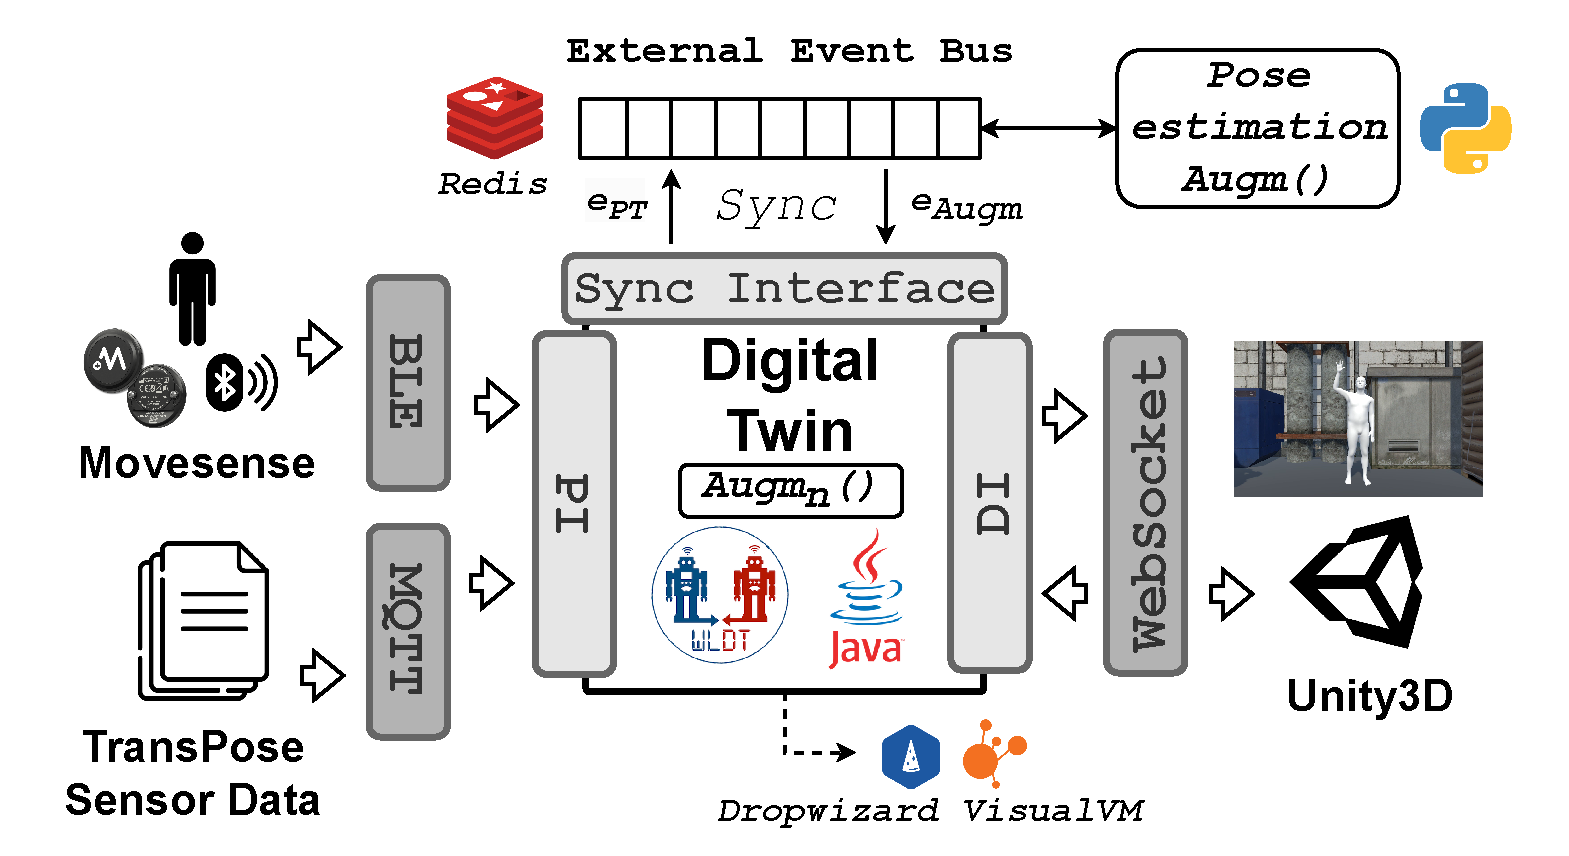
\includegraphics[width=0.9\textwidth]{figures/experimental_evaluation_scheme_new_industry.pdf}
    \caption{Experimental setup for evaluating the design of augmented digital twins for a pose estimation task.}
    \label{fig:augmentation-experimental-setup}
\end{figure}

A different experimental evaluation was conducted to validate the benefits of the modular design of augmentation proposed in \Cref{sec:dte:engineering-dt:dt-augmentation}.
%
The reference scenario involves the real-time monitoring of an industrial operator's movements within a manufacturing environment through a \ac{DT} whose state is augmented with pose estimation capabilities computed from inertial sensor data.

\Cref{fig:augmentation-experimental-setup} illustrates the experimental setup designed to evaluate the proposed augmentation function patterns within a \ac{DT}.
%
The \ac{DT} uses both physical devices and emulated traces, and embeds a machine learning model to estimate pose of the operator which is then visualized in a Unity3D\footnote{Unity: \url{https://unity.com/}} environment connected to the \ac{DT}.
%
This setup showcases how internal and external augmentation functions can be implemented in practice and what are the implications on the \ac{DT} performance.

The \ac{DT} acquires data from a Movesense Active sensor\footnote{Movesense: \url{https://www.movesense.com/movesense-active/}}: a wearable device featuring a 9-axis Inertial Measurement Unit (IMU) with accelerometer, gyroscope, and magnetometer capabilities, along with ECG and heart rate monitoring. This sensor, connected via Bluetooth Low Energy (BLE), allows for continuous tracking of physiological and motion-related data essential to represent the operator's state. Since the sensor can be configured to measure and send data with different sampling rates (13 Hz, 52 Hz, and 104 Hz) it was possible to test the \ac{DT} responsiveness under different conditions. 
%
For the reported experiments, the \ac{DT} has been deployed on a machine with an Intel i5-13600KF processor (5.1 GHz, 14 cores, 20 threads) and 32 GB of RAM and an RTX 4070ti GPU (12 GB GDDR6X).

%....................................................................
\subsubsection{Performance of Internal Augmentation Functions}
%....................................................................

To evaluate the performance of the augmentation functions, execution times, CPU usage, and memory consumption on the workstation were monitored.
%
Execution times were measured by testing various configurations.
The augmentation functions are implemented \emph{internally} in Java as periodic functions activated at a fixed period.
Each function computes the average of accelerometer values received from the Movesense sensor since the last activation.

In the first experiment, the activation interval of the functions was fixed (5 seconds).
Measurements of function execution time were taken using different sensor sampling frequencies (13, 52, and 104Hz) while varying the number of concurrently running functions (1, 3, and 5 functions).
%
\Cref{tab:AF_exec_time_fixed_act_period} presents the results from this experiment.
%
\begin{table}
    \setlength{\belowcaptionskip}{-6pt}
    \centering
    \begin{tabular}{p{4cm} p{2cm} p{2cm} p{2cm}}
    \hline
    \textbf{\#Augm.} & \textbf{13Hz} & \textbf{52Hz} & \textbf{104Hz} \\ \hline
    \textit{1 function} & 2.55ms & 6.58ms & 10.76ms \\ \hline
    \textit{3 functions} & 2.69ms & 6.54ms & 8.42ms \\ \hline
    \textit{5 functions} & 2.79ms & 6.79ms & 11.79ms \\ \hline\hline
    \end{tabular}
    \caption{Average AF execution time with fixed activation period (5s) varying sensor sampling frequency and number of simultaneous functions.}
    \label{tab:AF_exec_time_fixed_act_period}
\end{table}
%
The experimental evaluation of augmentation functions confirmed that even when multiple augmentation functions coexist within the same DT instance the \ac{DT} maintains good performance.

In the second experiment, the sampling frequency was fixed at 13 Hz.
%
In this setup, both the number of functions and their activation intervals were varied (1, 5, 10, and 30 seconds). The results from this experiment are detailed in \Cref{tab:AF_exec_time_fixed_sens_frequency}.
The \ac{DT} performance is still robust, with minimal increases in execution times even as the number of functions and activation intervals varied. This confirmed the system ability to handle multiple augmentation functions efficiently.
%
\begin{table}
    \centering
    \begin{tabular}{p{4cm} p{0.4cm} p{2cm} p{2cm} p{2cm} p{2cm}}
    \hline
    \textbf{\#Augm} & \multicolumn{1}{c}{\textbf{1s}} & \multicolumn{1}{c}{\textbf{5s}} & \multicolumn{1}{c}{\textbf{10s}} & \multicolumn{1}{c}{\textbf{30s}}\\ \hline
    \textit{1 function} & \multicolumn{1}{c}{1.70ms} & \multicolumn{1}{c}{2.05ms} & \multicolumn{1}{c}{4.17ms} & \multicolumn{1}{c}{12.64ms}\\ \hline
    \textit{3 functions} & \multicolumn{1}{c}{1.57ms} & \multicolumn{1}{c}{2.15ms} & \multicolumn{1}{c}{3.54ms} & \multicolumn{1}{c}{13.92ms}\\ \hline
    \textit{5 functions} & \multicolumn{1}{c}{2.37ms} & \multicolumn{1}{c}{2.20ms} & \multicolumn{1}{c}{5.93ms} & \multicolumn{1}{c}{11.1ms}\\ \hline\hline
    \end{tabular}
     \caption{Avg AF execution with fixed frequency at 13Hz varying number of functions and activation period.}
    \label{tab:AF_exec_time_fixed_sens_frequency}
\end{table}

A third experiment was conducted to further examine execution times with up to five Movesense sensors connected to the DT simultaneously. The function activation frequency was fixed at 5 seconds, while the number of connected devices and sampling frequencies were adjusted. \Cref{tab:AF_exec_time_multiple_devices} summarizes the outcomes. 

\begin{table}
    \centering
    \begin{tabular}{p{4cm} p{2cm} p{2cm} p{2cm}}
    \hline
    \textbf{\#Devices} & \textbf{13Hz} & \textbf{52Hz} & \textbf{104Hz} \\ \hline
    \textit{1 Device} & 3.60ms & 16.29ms & 32.59ms \\ \hline
    \textit{3 Devices} & 7.70ms & 46.61ms & 81.76ms \\ \hline
    \textit{4 Devices} & 18.56ms & 62.06ms & 111.71ms \\ \hline
    \textit{5 Devices} & 23.12ms & 75.68ms & 104.42ms \\ \hline\hline
    \end{tabular}
    \caption{Average AF execution time with multiple devices connected, varying sensor sampling frequency.}
    \label{tab:AF_exec_time_multiple_devices}
\end{table}

To evaluate the resource consumption of the augmentation functions running on the DT, a fourth experiment was performed using a single augmentation function with a 5-second activation interval.
In this setup, both CPU usage (as a percentage) and memory consumption (in MB) were measured across the three different sampling frequencies available with Movesense sensor (13, 52 and 104Hz).
%
The results for CPU and memory usage are summarized in \Cref{tab:AF_CPU_MEM_usage}. 
%
\begin{table}[t]
    \setlength{\belowcaptionskip}{-6pt}
    \centering
    \begin{tabular}{p{4cm} p{3cm} p{3cm}}
    \hline
    \textbf{Data Freq.} & \textbf{CPU\%} & \textbf{Mem [MB]} \\ \hline
    \textit{13Hz} & 0.72\% & 158MB \\ \hline
    \textit{52Hz} & 0.98\% & 157MB \\ \hline
    \textit{104Hz} & 1.16\% & 156MB \\ \hline\hline
    \end{tabular}
    \caption{Average AF CPU and memory usage with one function at a 5-second activation period and varying sensor sampling frequency.}
    \label{tab:AF_CPU_MEM_usage}
\end{table}
%
The results showed that the DT maintained efficient resource utilization across different sampling frequencies, further validating the architecture ability to support high-frequency data streams and complex computations even with multiple data sources and physical devices connected and managed by the \ac{DT}. These experiments collectively demonstrated that the feasibility of the proposed event-driven architecture for DT augmentation functions.

The architecture successfully supports augmentation of DT functionalities, providing timely insights and maintaining good performance, even under varied and demanding conditions.


\subsubsection{Pose Estimation with External Augmentation}

\begin{figure}
    \centering
    \begin{subfigure}{0.49\textwidth}
    \centering
        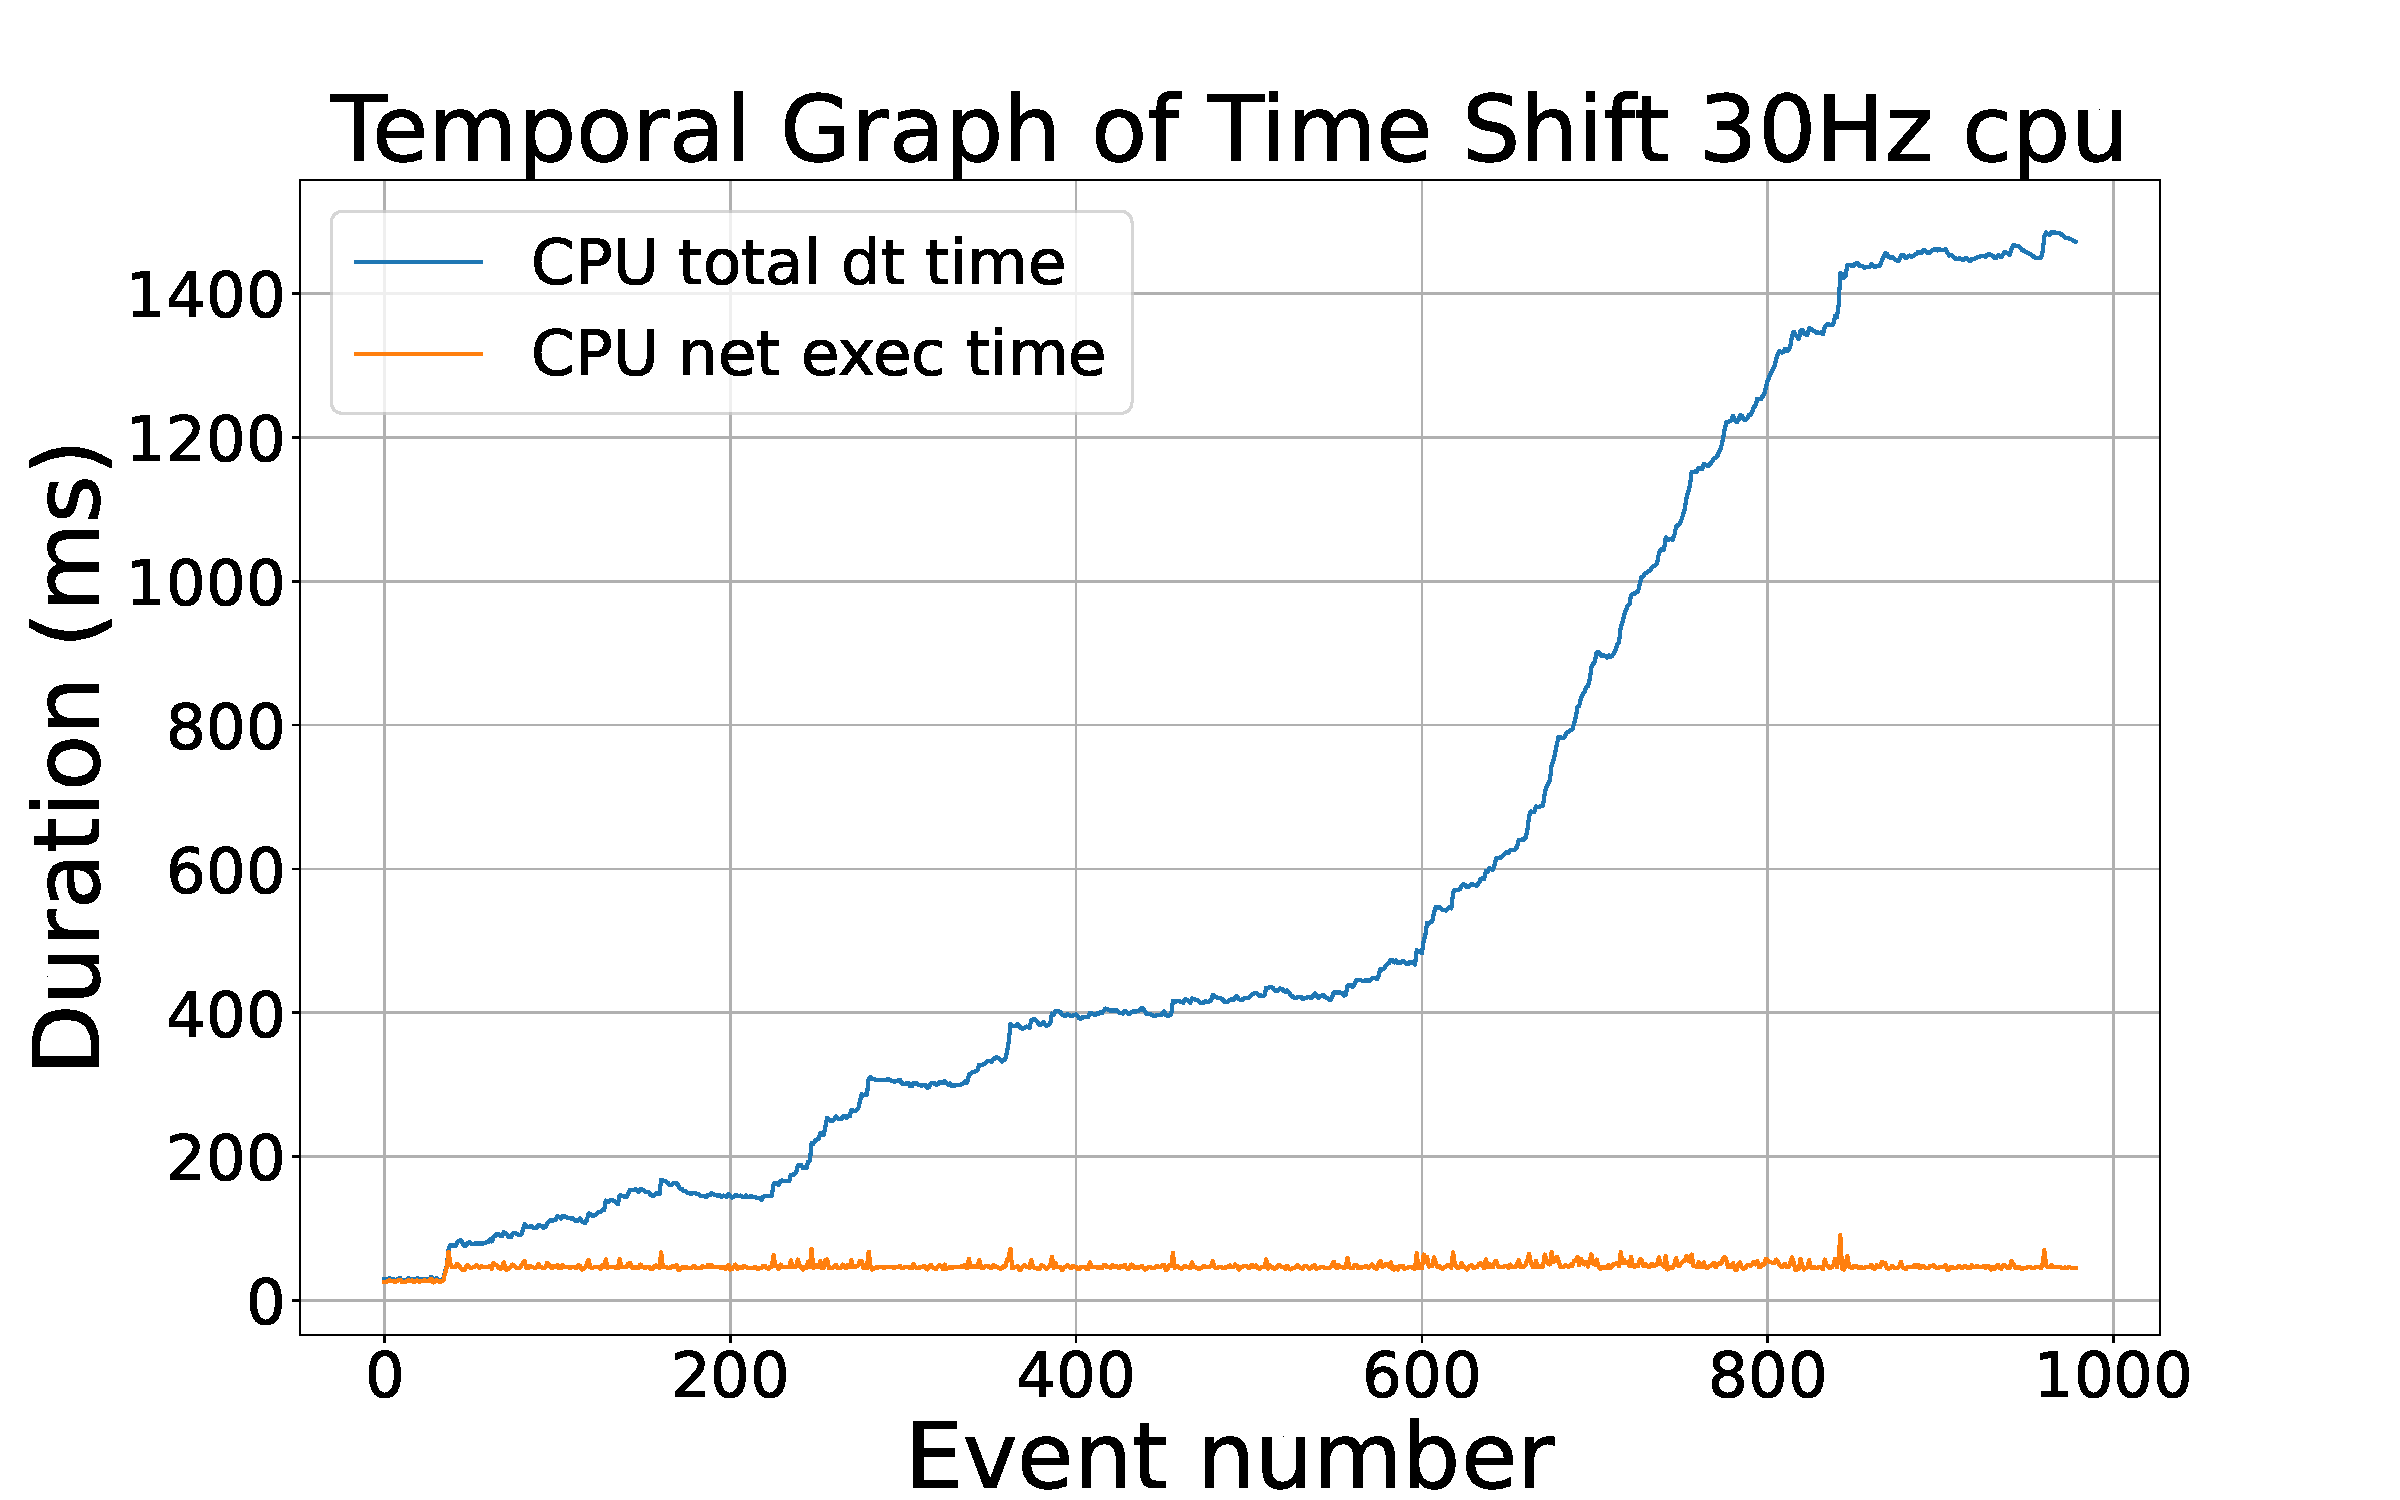
\includegraphics[width=\textwidth]{figures/temporal_graph_time_shift_30hz_cpu.pdf}
        \subcaption{}
        \label{fig:af_time_shift_30hz_cpu}
    \end{subfigure}
    \hfill
    \begin{subfigure}{0.49\textwidth}
    \centering
        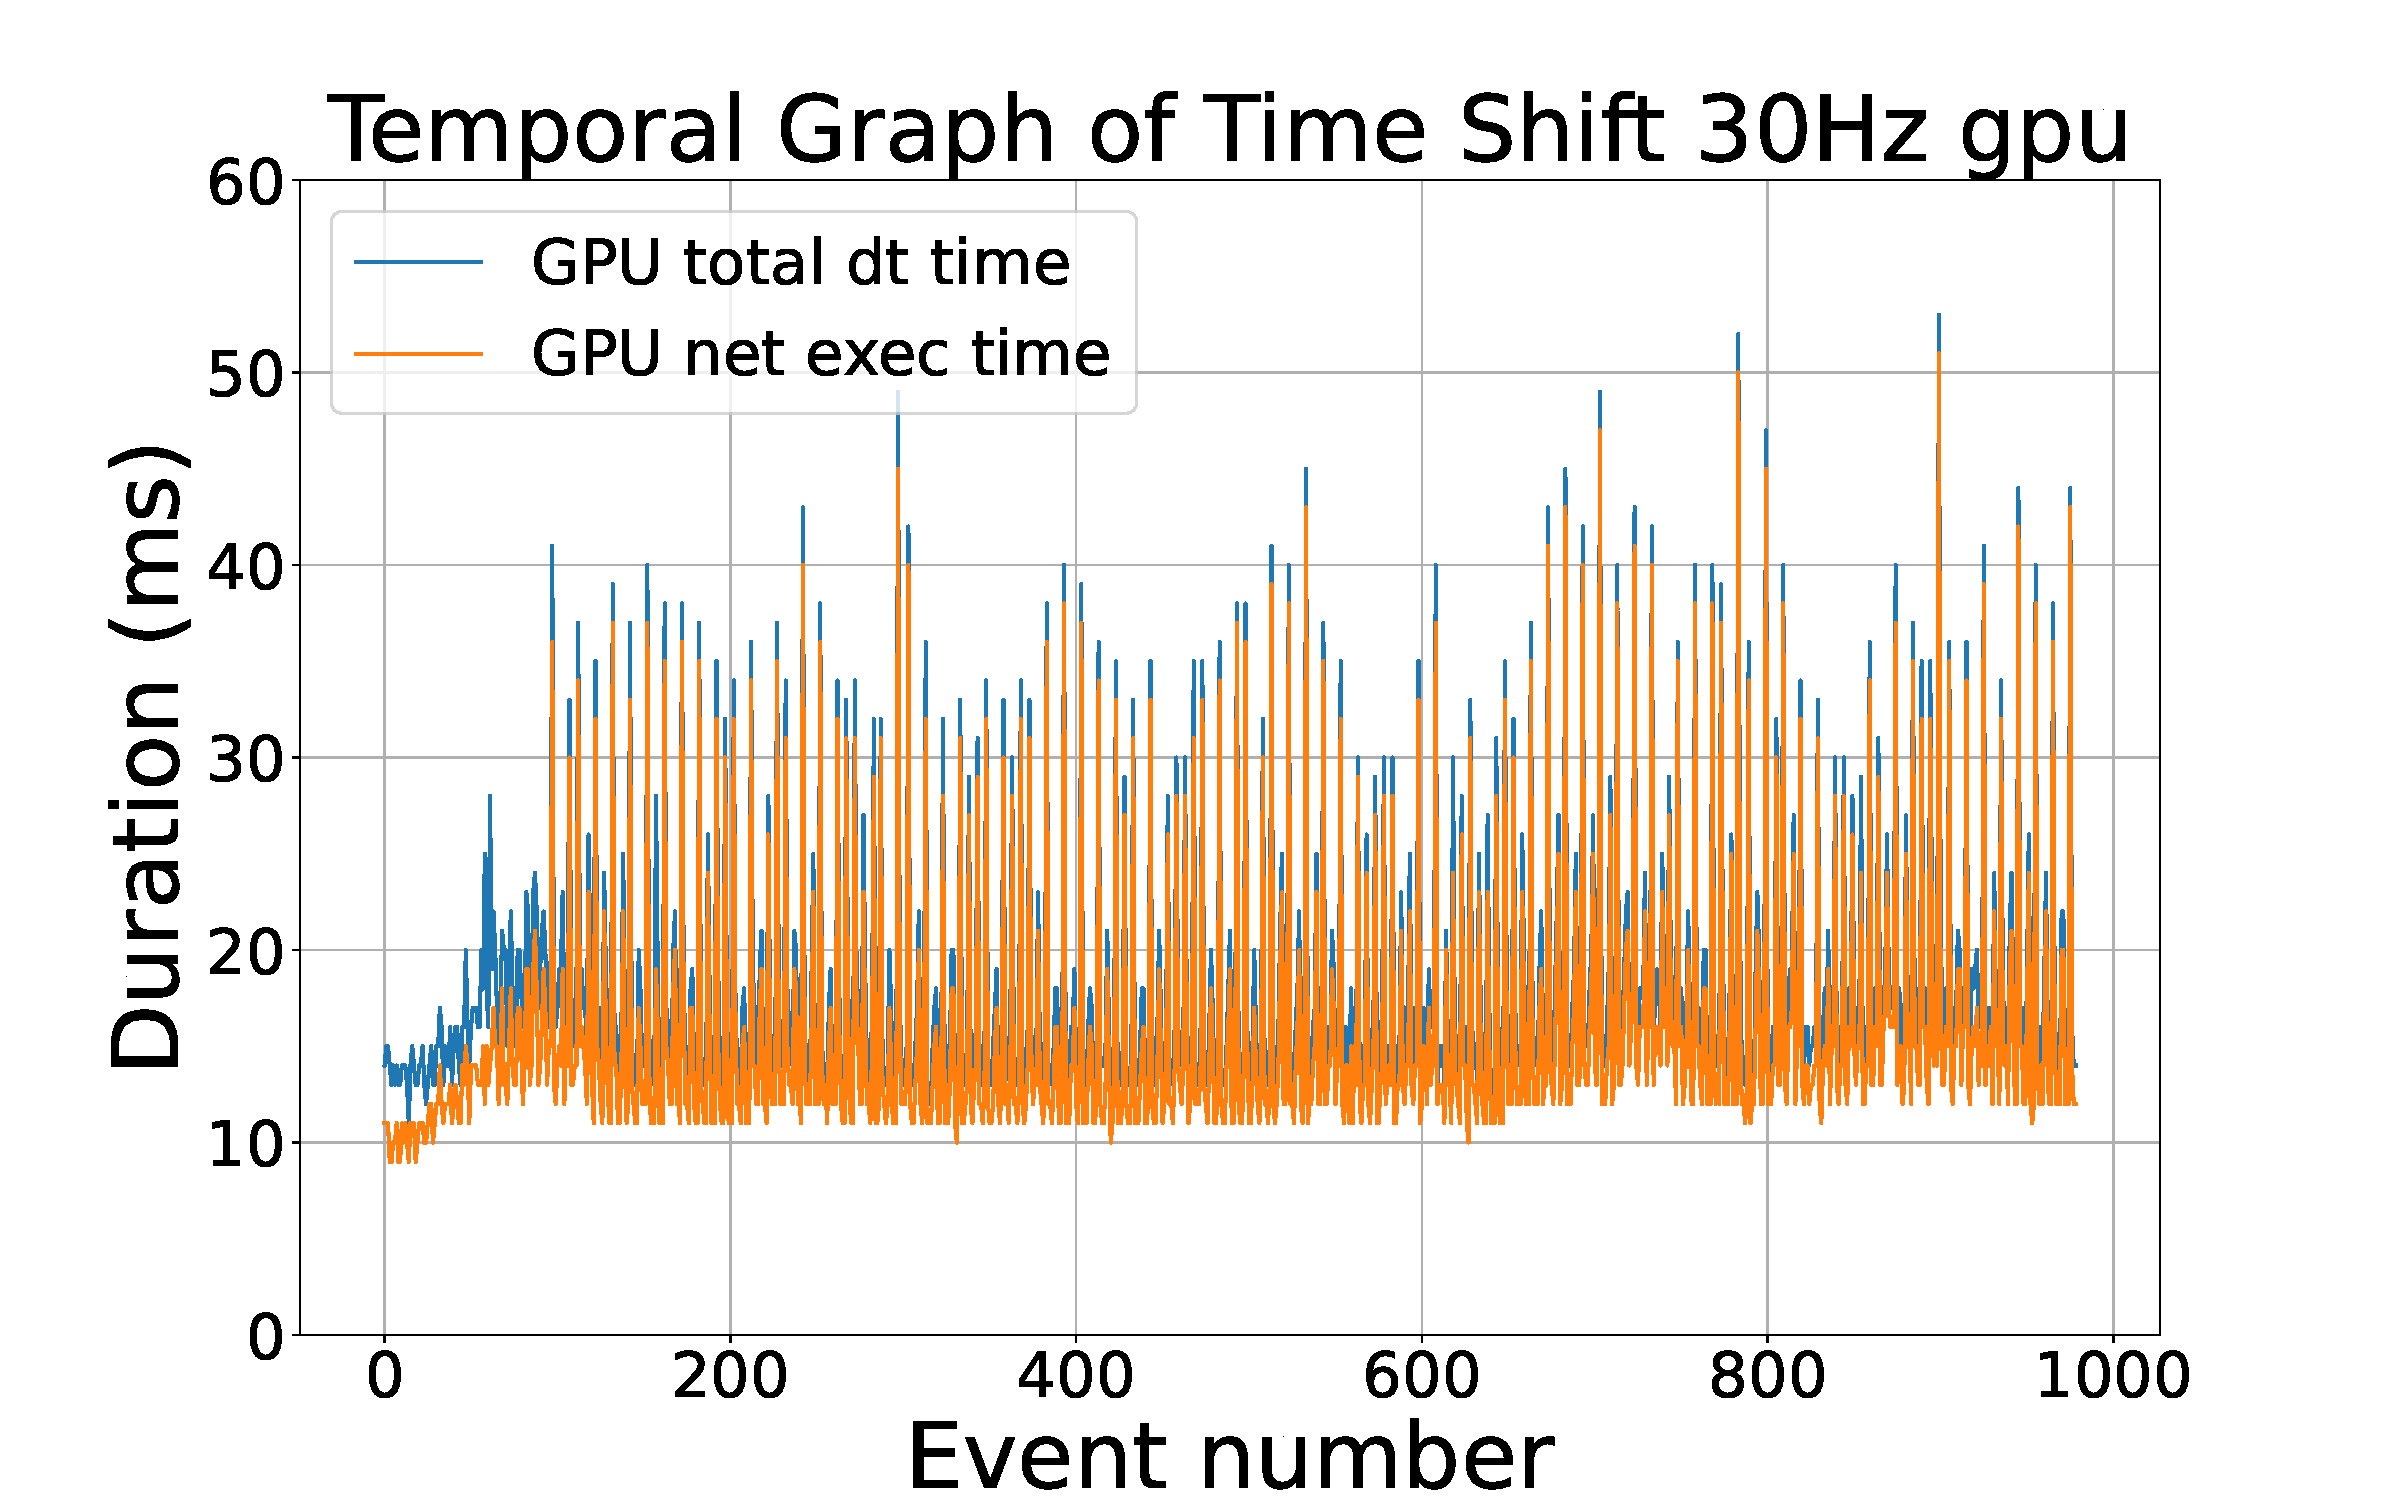
\includegraphics[width=\textwidth]{figures/temporal_graph_time_shift_30hz_gpu.pdf}
        \subcaption{}
        \label{fig:af_time_shift_30hz_gpu}
    \end{subfigure}
    \caption{Pose estimation latency computed within the DT compared to standalone execution, using the CPU (a) and using the GPU (b).}
    \label{fig:af_results}
\end{figure}

For the implementation of the pose estimation \ac{DT} feature,
the augmentation function is implemented externally using a Recurrent Neural Network from the TransPose project~\cite{TransPoseSIGGRAPH2021} using accelerometer data from six inertial sensors positioned on the operator's body to compute its position.
%
As shown in \Cref{fig:augmentation-experimental-setup} the original dataset of the project is used to emulate traces that are sent with a 30Hz frequency to the \ac{DT} through its physical interface using MQTT.
%
The augmentation function operates externally, running in parallel with the DT. Data exchange occurs via a Redis event bus, and once the position is determined, the \ac{DT} shadowing function publishes the result through the digital interface using a WebSocket to apply the inferred pose on a 3D model of a person in a Unity3D environment for visualization purposes.

The latency between data transmission and the reception of the estimated pose by the Unity3D application is measured to assess the performance of the external augmentation function.
%
First the neural network is executed using only the CPU, and then with GPU acceleration, to evaluate the impact of consciously allocating resources to augmentation functions.

Both the neural network model and the DT are executed on the same workstation. \Cref{fig:af_time_shift_30hz_cpu} illustrates the total latency introduced by the DT and the model compared with the latency associated to the same function executed outside the DT.
%
With CPU-only execution, the overall delay increases as the model cannot keep up, causing event queue buildup and increased latency. 
As shown in \Cref{fig:af_time_shift_30hz_gpu}, with the allocation of GPU resources the delay between transmission and reception remains stable over time, with most latency now attributed to model execution rather than DT processes.

This experiment demonstrates that the proposed model for the augmentation functions effectively supports developers in distributing the computational load on dedicated resources, thus improving the overall \ac{DT} performances. 

In conclusion, the experimental evaluation demonstrates that the proposed event-driven architecture for DT augmentation functions is both feasible and efficient.
The internal, external, and hybrid augmentation strategies offer flexibility, enabling real-time data processing and complex computations.
The architecture supports high-frequency data streams and provides timely insights, making it suitable for different applications.


%==============================
\section{Final Remarks}
%==============================

This chapter presents contributions to the engineering of \acp{DT} focusing on key challenges in the modeling and implementation of \acp{DT} as active components in an \ac{IoT} system, capable of integrating heterogeneous data sources, managing their synchronization with the \ac{PA} lifecycle and provide augmented functionalities. 

Despite the target scenario used for validation being an industrial manufacturing setting, emulated through a lab-scale production line, the proposed architectural framework and patterns are general and can be applied to other domains.
%
Indeed, the \ac{WLDT} framework, implementing the functionalities described in this chapter, has been used in different contexts such as smart-cities and healthcare. 

The chapter addresses the research question:

\paragraph{\ref{rq:1} How can we engineer \acp{DT} to integrate heterogeneous data sources and provide an up-to-date uniform representation of the mirrored assets?}
%
The modular architecture grounded on the concept of \acp{PhA} and \acp{DiA} effectively decouples the complexities of physical and digital environments from the core responsibilities of the \ac{DT}.
%
This enables integration of heterogeneous data sources by means of reusable components, simplifying the development of \acp{DT} and promoting interoperability.
%
Furthermore, the lifecycle management managed at the \ac{DT} level ensures that domain-specific synchronization requirements can be validated and enforced, providing applications with accurate and timely information about the state of the \ac{PA}.
%
Finally, the modular approach to \ac{DT} augmentation allows for the flexible integration of additional functionalities, either internally or externally, without impacting the core shadowing responsibilities of the \ac{DT}.
